\documentclass[twoside]{book}

% Packages required by doxygen
\usepackage{fixltx2e}
\usepackage{calc}
\usepackage{doxygen}
\usepackage[export]{adjustbox} % also loads graphicx
\usepackage{graphicx}
\usepackage[utf8]{inputenc}
\usepackage{makeidx}
\usepackage{multicol}
\usepackage{multirow}
\PassOptionsToPackage{warn}{textcomp}
\usepackage{textcomp}
\usepackage[nointegrals]{wasysym}
\usepackage[table]{xcolor}

% Font selection
\usepackage[T1]{fontenc}
\usepackage[scaled=.90]{helvet}
\usepackage{courier}
\usepackage{amssymb}
\usepackage{sectsty}
\renewcommand{\familydefault}{\sfdefault}
\allsectionsfont{%
  \fontseries{bc}\selectfont%
  \color{darkgray}%
}
\renewcommand{\DoxyLabelFont}{%
  \fontseries{bc}\selectfont%
  \color{darkgray}%
}
\newcommand{\+}{\discretionary{\mbox{\scriptsize$\hookleftarrow$}}{}{}}

% Page & text layout
\usepackage{geometry}
\geometry{%
  a4paper,%
  top=2.5cm,%
  bottom=2.5cm,%
  left=2.5cm,%
  right=2.5cm%
}
\tolerance=750
\hfuzz=15pt
\hbadness=750
\setlength{\emergencystretch}{15pt}
\setlength{\parindent}{0cm}
\setlength{\parskip}{3ex plus 2ex minus 2ex}
\makeatletter
\renewcommand{\paragraph}{%
  \@startsection{paragraph}{4}{0ex}{-1.0ex}{1.0ex}{%
    \normalfont\normalsize\bfseries\SS@parafont%
  }%
}
\renewcommand{\subparagraph}{%
  \@startsection{subparagraph}{5}{0ex}{-1.0ex}{1.0ex}{%
    \normalfont\normalsize\bfseries\SS@subparafont%
  }%
}
\makeatother

% Headers & footers
\usepackage{fancyhdr}
\pagestyle{fancyplain}
\fancyhead[LE]{\fancyplain{}{\bfseries\thepage}}
\fancyhead[CE]{\fancyplain{}{}}
\fancyhead[RE]{\fancyplain{}{\bfseries\leftmark}}
\fancyhead[LO]{\fancyplain{}{\bfseries\rightmark}}
\fancyhead[CO]{\fancyplain{}{}}
\fancyhead[RO]{\fancyplain{}{\bfseries\thepage}}
\fancyfoot[LE]{\fancyplain{}{}}
\fancyfoot[CE]{\fancyplain{}{}}
\fancyfoot[RE]{\fancyplain{}{\bfseries\scriptsize Generated by Doxygen }}
\fancyfoot[LO]{\fancyplain{}{\bfseries\scriptsize Generated by Doxygen }}
\fancyfoot[CO]{\fancyplain{}{}}
\fancyfoot[RO]{\fancyplain{}{}}
\renewcommand{\footrulewidth}{0.4pt}
\renewcommand{\chaptermark}[1]{%
  \markboth{#1}{}%
}
\renewcommand{\sectionmark}[1]{%
  \markright{\thesection\ #1}%
}

% Indices & bibliography
\usepackage{natbib}
\usepackage[titles]{tocloft}
\setcounter{tocdepth}{3}
\setcounter{secnumdepth}{5}
\makeindex

% Hyperlinks (required, but should be loaded last)
\usepackage{ifpdf}
\ifpdf
  \usepackage[pdftex,pagebackref=true]{hyperref}
\else
  \usepackage[ps2pdf,pagebackref=true]{hyperref}
\fi
\hypersetup{%
  colorlinks=true,%
  linkcolor=blue,%
  citecolor=blue,%
  unicode%
}

% Custom commands
\newcommand{\clearemptydoublepage}{%
  \newpage{\pagestyle{empty}\cleardoublepage}%
}

\usepackage{caption}
\captionsetup{labelsep=space,justification=centering,font={bf},singlelinecheck=off,skip=4pt,position=top}

%===== C O N T E N T S =====

\begin{document}

% Titlepage & ToC
\hypersetup{pageanchor=false,
             bookmarksnumbered=true,
             pdfencoding=unicode
            }
\pagenumbering{alph}
\begin{titlepage}
\vspace*{7cm}
\begin{center}%
{\Large C\+Turtle }\\
\vspace*{1cm}
{\large Generated by Doxygen 1.8.13}\\
\end{center}
\end{titlepage}
\clearemptydoublepage
\pagenumbering{roman}
\tableofcontents
\clearemptydoublepage
\pagenumbering{arabic}
\hypersetup{pageanchor=true}

%--- Begin generated contents ---
\chapter{Todo List}
\label{todo}
\Hypertarget{todo}

\begin{DoxyRefList}
\item[Member \mbox{\hyperlink{classcturtle_1_1InteractiveTurtleScreen_a1c666afe65211cf9eedaffa17206a697}{cturtle::Interactive\+Turtle\+Screen::mode}} (Screen\+Mode mode)]\label{todo__todo000001}%
\Hypertarget{todo__todo000001}%
Refine this documentation. 
\end{DoxyRefList}
\chapter{Hierarchical Index}
\section{Class Hierarchy}
This inheritance list is sorted roughly, but not completely, alphabetically\+:\begin{DoxyCompactList}
\item \contentsline{section}{cturtle\+:\+:Abstract\+Drawable\+Object}{\pageref{classcturtle_1_1AbstractDrawableObject}}{}
\begin{DoxyCompactList}
\item \contentsline{section}{cturtle\+:\+:Circle}{\pageref{classcturtle_1_1Circle}}{}
\item \contentsline{section}{cturtle\+:\+:Compound\+Polygon}{\pageref{classcturtle_1_1CompoundPolygon}}{}
\item \contentsline{section}{cturtle\+:\+:Line}{\pageref{classcturtle_1_1Line}}{}
\item \contentsline{section}{cturtle\+:\+:Polygon}{\pageref{classcturtle_1_1Polygon}}{}
\item \contentsline{section}{cturtle\+:\+:Sprite}{\pageref{classcturtle_1_1Sprite}}{}
\item \contentsline{section}{cturtle\+:\+:Text}{\pageref{classcturtle_1_1Text}}{}
\end{DoxyCompactList}
\item \contentsline{section}{cturtle\+:\+:Abstract\+Turtle\+Screen}{\pageref{classcturtle_1_1AbstractTurtleScreen}}{}
\begin{DoxyCompactList}
\item \contentsline{section}{cturtle\+:\+:Interactive\+Turtle\+Screen}{\pageref{classcturtle_1_1InteractiveTurtleScreen}}{}
\end{DoxyCompactList}
\item \contentsline{section}{cturtle\+:\+:Color}{\pageref{classcturtle_1_1Color}}{}
\item \contentsline{section}{cturtle\+:\+:Input\+Event}{\pageref{structcturtle_1_1InputEvent}}{}
\item \contentsline{section}{cturtle\+:\+:ivec2}{\pageref{structcturtle_1_1ivec2}}{}
\item \contentsline{section}{cturtle\+:\+:Pen\+State}{\pageref{structcturtle_1_1PenState}}{}
\item \contentsline{section}{cturtle\+:\+:Scene\+Object}{\pageref{structcturtle_1_1SceneObject}}{}
\item \contentsline{section}{cturtle\+:\+:Transform}{\pageref{classcturtle_1_1Transform}}{}
\item \contentsline{section}{cturtle\+:\+:Turtle}{\pageref{classcturtle_1_1Turtle}}{}
\end{DoxyCompactList}

\chapter{Class Index}
\doxysection{Class List}
Here are the classes, structs, unions and interfaces with brief descriptions\+:\begin{DoxyCompactList}
\item\contentsline{section}{\mbox{\hyperlink{classcturtle_1_1AbstractDrawableObject}{cturtle\+::\+Abstract\+Drawable\+Object}} \\*\mbox{\hyperlink{classcturtle_1_1AbstractDrawableObject}{Abstract\+Drawable\+Object}} is a base class, intended to be inherited from by all drawable objects. This class just contains a simple virtual drawing function, intended to be inherited from and to overload the draw function. This allows for the storage of drawable geometry/etc and attributes in a generic fashion }{\pageref{classcturtle_1_1AbstractDrawableObject}}{}
\item\contentsline{section}{\mbox{\hyperlink{classcturtle_1_1AbstractTurtleScreen}{cturtle\+::\+Abstract\+Turtle\+Screen}} \\*Abstract type for most turtle functionality. It intentionally excludes all input/output functionality, allowing for two intended derivates\+: an \char`\"{}interactive\char`\"{} screen, vs an \char`\"{}offline rendering\char`\"{} screen. The \mbox{\hyperlink{classcturtle_1_1Turtle}{Turtle}} class doesn\textquotesingle{}t care which one it gets attached to }{\pageref{classcturtle_1_1AbstractTurtleScreen}}{}
\item\contentsline{section}{\mbox{\hyperlink{classcturtle_1_1BitmapFont}{cturtle\+::\+Bitmap\+Font}} \\*The Bitmap Font represents monospaced font image files that covers a range of lower ASCII. The default font, for example, covers 32-\/127 (e.\+g, char 32 to char 127). This is a particularly naive implementation of bitmap fonts, however, all basic properties required are here }{\pageref{classcturtle_1_1BitmapFont}}{}
\item\contentsline{section}{\mbox{\hyperlink{classcturtle_1_1Circle}{cturtle\+::\+Circle}} \\*Holds a radius and total number of steps, used to generate and draw a circles geometry }{\pageref{classcturtle_1_1Circle}}{}
\item\contentsline{section}{\mbox{\hyperlink{classcturtle_1_1Color}{cturtle\+::\+Color}} \\*The primary representation of \mbox{\hyperlink{classcturtle_1_1Color}{Color}} for this library. Represented as a simple RGB color composed of unsigned bytes, \mbox{\hyperlink{classcturtle_1_1Color}{Color}} objects can be referenced by string and by packed integer }{\pageref{classcturtle_1_1Color}}{}
\item\contentsline{section}{\mbox{\hyperlink{classcturtle_1_1CompoundPolygon}{cturtle\+::\+Compound\+Polygon}} \\*Compound \mbox{\hyperlink{classcturtle_1_1Polygon}{Polygon}} instance is composed from a number of smaller parts, which are each derived from \mbox{\hyperlink{classcturtle_1_1AbstractDrawableObject}{Abstract\+Drawable\+Object}}. Compound Polygons can have a variety of attachments. After the parts are assembled, the polygon is essentially read-\/only. These can be used to assemble several pieces of geometry into one object. These objects are self-\/contained and have ownership of all \mbox{\hyperlink{classcturtle_1_1AbstractDrawableObject}{Abstract\+Drawable\+Object}} instances they contain }{\pageref{classcturtle_1_1CompoundPolygon}}{}
\item\contentsline{section}{\mbox{\hyperlink{structcturtle_1_1InputEvent}{cturtle\+::\+Input\+Event}} \\*The internally-\/used representation of an Input Event. Contains information pertaining to keyboard and mouse events, as well as callback pointers for either case }{\pageref{structcturtle_1_1InputEvent}}{}
\item\contentsline{section}{\mbox{\hyperlink{classcturtle_1_1InteractiveTurtleScreen}{cturtle\+::\+Interactive\+Turtle\+Screen}} \\*Holds and maintains facilities in relation to displaying \textbackslash{} turtles and consuming input events from users through callbacks. This includes holding the actual data for a given scene after being populated by \mbox{\hyperlink{classcturtle_1_1Turtle}{Turtle}}. It layers draw calls in the order they are called, independent of whatever \mbox{\hyperlink{classcturtle_1_1Turtle}{Turtle}} object creates it }{\pageref{classcturtle_1_1InteractiveTurtleScreen}}{}
\item\contentsline{section}{\mbox{\hyperlink{structcturtle_1_1ivec2}{cturtle\+::ivec2}} \\*Represents a coordinate pair (e.\+g, x \& y) This class is represented as a low-\/precision point, because this data type tends to be most easily drawn to a simple canvas }{\pageref{structcturtle_1_1ivec2}}{}
\item\contentsline{section}{\mbox{\hyperlink{classcturtle_1_1Line}{cturtle\+::\+Line}} \\*Holds two points and the functionality to draw a line between them on a specified canvas }{\pageref{classcturtle_1_1Line}}{}
\item\contentsline{section}{\mbox{\hyperlink{structcturtle_1_1PenState}{cturtle\+::\+Pen\+State}} \\*The Pen State structure Holds all pen attributes, which are grouped in this way to allow stack-\/based undo for \mbox{\hyperlink{classcturtle_1_1Turtle}{Turtle}} objects. Instances of this object are self-\/contained, and has ownership of all objects and memory referenced by itself }{\pageref{structcturtle_1_1PenState}}{}
\item\contentsline{section}{\mbox{\hyperlink{classcturtle_1_1Polygon}{cturtle\+::\+Polygon}} \\*The polygon class merely holds a vector of points and a function to draw this series to an image. Please note that the contained series of points must be in either clockwise(\+CW) or counterclockwise(\+CCW) order! }{\pageref{classcturtle_1_1Polygon}}{}
\item\contentsline{section}{\mbox{\hyperlink{structcturtle_1_1SceneObject}{cturtle\+::\+Scene\+Object}} \\*Turtles append Scene Objects to a list to keep track of what it has drawn (a history). \mbox{\hyperlink{structcturtle_1_1SceneObject}{Scene\+Object}} holds a description of something that needs to be on the screen. It\textquotesingle{}s a general object which encompasses ALL things that can be on screen, ranging from stamps, misc. geometry, and strings }{\pageref{structcturtle_1_1SceneObject}}{}
\item\contentsline{section}{\mbox{\hyperlink{classcturtle_1_1Sprite}{cturtle\+::\+Sprite}} \\*Selection of a larger image. This class ignores color in favor of color provided by the image the sprite corresponds to }{\pageref{classcturtle_1_1Sprite}}{}
\item\contentsline{section}{\mbox{\hyperlink{classcturtle_1_1Text}{cturtle\+::\+Text}} \\*Basic string that is drawn on the screen }{\pageref{classcturtle_1_1Text}}{}
\item\contentsline{section}{\mbox{\hyperlink{classcturtle_1_1Transform}{cturtle\+::\+Transform}} \\*Myriad of functions to simply transform points. This class it the backbone of almost all cartesian plane math in CTurtle. An adapted 3x3 matrix of the following link\+: \href{http://www.opengl-tutorial.org/beginners-tutorials/tutorial-3-matrices/}{\texttt{ http\+://www.\+opengl-\/tutorial.\+org/beginners-\/tutorials/tutorial-\/3-\/matrices/}} }{\pageref{classcturtle_1_1Transform}}{}
\item\contentsline{section}{\mbox{\hyperlink{classcturtle_1_1Turtle}{cturtle\+::\+Turtle}} \\*The \mbox{\hyperlink{classcturtle_1_1Turtle}{Turtle}} Class Symbolically represents a turtle that runs around a screen that has a paint brush attached to its tail. The tail can be in two states; up and down. As the turtle moves forwards, backwards, left, and right, it can draw shapes and outlines, write text, and stamp itself onto whatever surface it\textquotesingle{}s walking/crawling on (In this case, it\textquotesingle{}s walking on a Turtle\+Screen) }{\pageref{classcturtle_1_1Turtle}}{}
\end{DoxyCompactList}

\chapter{Class Documentation}
\hypertarget{classcturtle_1_1AbstractDrawableObject}{}\section{cturtle\+:\+:Abstract\+Drawable\+Object Class Reference}
\label{classcturtle_1_1AbstractDrawableObject}\index{cturtle\+::\+Abstract\+Drawable\+Object@{cturtle\+::\+Abstract\+Drawable\+Object}}


\hyperlink{classcturtle_1_1AbstractDrawableObject}{Abstract\+Drawable\+Object} is a base class, intended to be inherited from by all drawable objects. This class just contains a simple virtual drawing function, intended to be inherited from and to overload the draw function. This allows for the storage of drawable geometry/etc and attributes in a generic fashion.  




{\ttfamily \#include $<$C\+Turtle.\+hpp$>$}



Inheritance diagram for cturtle\+:\+:Abstract\+Drawable\+Object\+:\nopagebreak
\begin{figure}[H]
\begin{center}
\leavevmode
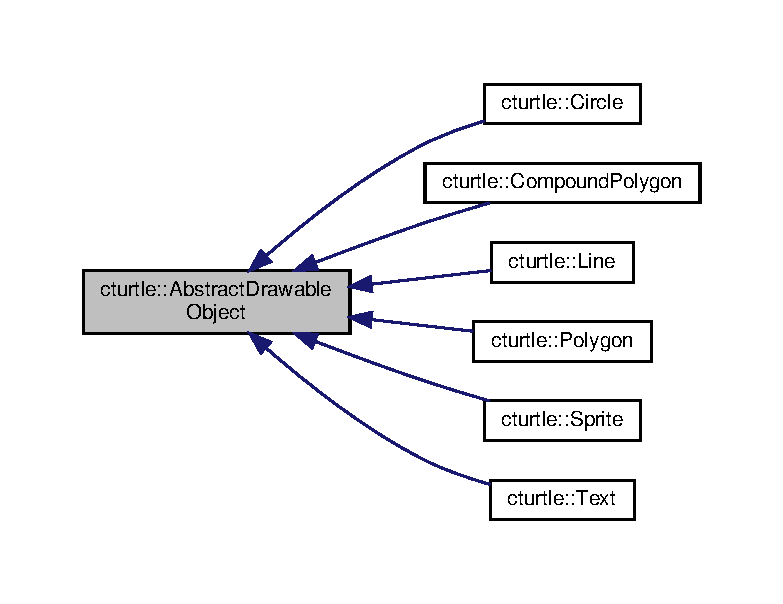
\includegraphics[width=350pt]{classcturtle_1_1AbstractDrawableObject__inherit__graph}
\end{center}
\end{figure}


Collaboration diagram for cturtle\+:\+:Abstract\+Drawable\+Object\+:\nopagebreak
\begin{figure}[H]
\begin{center}
\leavevmode
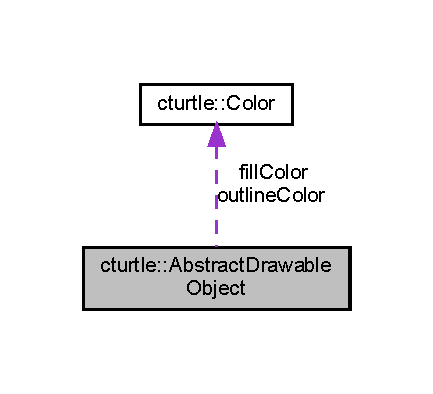
\includegraphics[width=208pt]{classcturtle_1_1AbstractDrawableObject__coll__graph}
\end{center}
\end{figure}
\subsection*{Public Member Functions}
\begin{DoxyCompactItemize}
\item 
\mbox{\Hypertarget{classcturtle_1_1AbstractDrawableObject_ab341cf2b8c9bf6cafd11195e21b8ed21}\label{classcturtle_1_1AbstractDrawableObject_ab341cf2b8c9bf6cafd11195e21b8ed21}} 
\hyperlink{classcturtle_1_1AbstractDrawableObject_ab341cf2b8c9bf6cafd11195e21b8ed21}{Abstract\+Drawable\+Object} ()
\begin{DoxyCompactList}\small\item\em Empty default constructor. \end{DoxyCompactList}\item 
\mbox{\Hypertarget{classcturtle_1_1AbstractDrawableObject_ae2f6b7c2e982b772779ec2957003b028}\label{classcturtle_1_1AbstractDrawableObject_ae2f6b7c2e982b772779ec2957003b028}} 
virtual \hyperlink{classcturtle_1_1AbstractDrawableObject_ae2f6b7c2e982b772779ec2957003b028}{$\sim$\+Abstract\+Drawable\+Object} ()
\begin{DoxyCompactList}\small\item\em Empty-- virtual-- default de-\/constructor. \end{DoxyCompactList}\item 
\mbox{\Hypertarget{classcturtle_1_1AbstractDrawableObject_acff3437e999d281773b66e6cf2115372}\label{classcturtle_1_1AbstractDrawableObject_acff3437e999d281773b66e6cf2115372}} 
virtual \hyperlink{classcturtle_1_1AbstractDrawableObject}{Abstract\+Drawable\+Object} $\ast$ \hyperlink{classcturtle_1_1AbstractDrawableObject_acff3437e999d281773b66e6cf2115372}{copy} () const =0
\begin{DoxyCompactList}\small\item\em Returns a pointer to a copy of this drawable object, allocated with N\+EW. Result Must be deleted at the responsibility of the invoker. \end{DoxyCompactList}\item 
virtual void \hyperlink{classcturtle_1_1AbstractDrawableObject_a7b1ad1e9743d343e0fe577de3978bdad}{draw} (const \hyperlink{classcturtle_1_1Transform}{Transform} \&t, Image \&img\+Ref) const =0
\begin{DoxyCompactList}\small\item\em This function is intended to draw all applicable geometry in this object to the specified image, with the specified transform, with the specified color. This function is intended to be overloaded by child classes to draw applicable geometry to an image, acting as a canvas. \end{DoxyCompactList}\end{DoxyCompactItemize}
\subsection*{Public Attributes}
\begin{DoxyCompactItemize}
\item 
\hyperlink{classcturtle_1_1Color}{Color} \hyperlink{classcturtle_1_1AbstractDrawableObject_a37d635a02ad3e5206a6eb99b7b5f1963}{fill\+Color}
\item 
\hyperlink{classcturtle_1_1Color}{Color} \hyperlink{classcturtle_1_1AbstractDrawableObject_abd04640855e7623bb84b52babd8b32b6}{outline\+Color}
\item 
int \hyperlink{classcturtle_1_1AbstractDrawableObject_aeffaecc245057e9a42e5688671a77f52}{outline\+Width} = 0
\end{DoxyCompactItemize}


\subsection{Detailed Description}
\hyperlink{classcturtle_1_1AbstractDrawableObject}{Abstract\+Drawable\+Object} is a base class, intended to be inherited from by all drawable objects. This class just contains a simple virtual drawing function, intended to be inherited from and to overload the draw function. This allows for the storage of drawable geometry/etc and attributes in a generic fashion. 

\subsection{Member Function Documentation}
\mbox{\Hypertarget{classcturtle_1_1AbstractDrawableObject_a7b1ad1e9743d343e0fe577de3978bdad}\label{classcturtle_1_1AbstractDrawableObject_a7b1ad1e9743d343e0fe577de3978bdad}} 
\index{cturtle\+::\+Abstract\+Drawable\+Object@{cturtle\+::\+Abstract\+Drawable\+Object}!draw@{draw}}
\index{draw@{draw}!cturtle\+::\+Abstract\+Drawable\+Object@{cturtle\+::\+Abstract\+Drawable\+Object}}
\subsubsection{\texorpdfstring{draw()}{draw()}}
{\footnotesize\ttfamily virtual void cturtle\+::\+Abstract\+Drawable\+Object\+::draw (\begin{DoxyParamCaption}\item[{const \hyperlink{classcturtle_1_1Transform}{Transform} \&}]{t,  }\item[{Image \&}]{img\+Ref }\end{DoxyParamCaption}) const\hspace{0.3cm}{\ttfamily [pure virtual]}}



This function is intended to draw all applicable geometry in this object to the specified image, with the specified transform, with the specified color. This function is intended to be overloaded by child classes to draw applicable geometry to an image, acting as a canvas. 


\begin{DoxyParams}{Parameters}
{\em t} & The transform at which to draw the geometry. \\
\hline
{\em img\+Ref} & The canvas on which to draw. \\
\hline
{\em c} & The color with to draw the geometry. \\
\hline
\end{DoxyParams}


Implemented in \hyperlink{classcturtle_1_1CompoundPolygon_aee485a61907d0a9c135344eadd5c52ad}{cturtle\+::\+Compound\+Polygon}, \hyperlink{classcturtle_1_1Sprite_a7b57808acc51a2610b7d33f542a7f838}{cturtle\+::\+Sprite}, \hyperlink{classcturtle_1_1Polygon_a4a0b6c44656957b141b74bd5c1542622}{cturtle\+::\+Polygon}, \hyperlink{classcturtle_1_1Circle_a7c95f8f4d126e38661e4ee94be58a8c4}{cturtle\+::\+Circle}, \hyperlink{classcturtle_1_1Line_a25ac5b4024bf9209d324b6f8c16affaf}{cturtle\+::\+Line}, and \hyperlink{classcturtle_1_1Text_a80003e4c447def1c7de8daf29a8fc5ec}{cturtle\+::\+Text}.



\subsection{Member Data Documentation}
\mbox{\Hypertarget{classcturtle_1_1AbstractDrawableObject_a37d635a02ad3e5206a6eb99b7b5f1963}\label{classcturtle_1_1AbstractDrawableObject_a37d635a02ad3e5206a6eb99b7b5f1963}} 
\index{cturtle\+::\+Abstract\+Drawable\+Object@{cturtle\+::\+Abstract\+Drawable\+Object}!fill\+Color@{fill\+Color}}
\index{fill\+Color@{fill\+Color}!cturtle\+::\+Abstract\+Drawable\+Object@{cturtle\+::\+Abstract\+Drawable\+Object}}
\subsubsection{\texorpdfstring{fill\+Color}{fillColor}}
{\footnotesize\ttfamily \hyperlink{classcturtle_1_1Color}{Color} cturtle\+::\+Abstract\+Drawable\+Object\+::fill\+Color}

The internal fill color of the circle. \mbox{\Hypertarget{classcturtle_1_1AbstractDrawableObject_abd04640855e7623bb84b52babd8b32b6}\label{classcturtle_1_1AbstractDrawableObject_abd04640855e7623bb84b52babd8b32b6}} 
\index{cturtle\+::\+Abstract\+Drawable\+Object@{cturtle\+::\+Abstract\+Drawable\+Object}!outline\+Color@{outline\+Color}}
\index{outline\+Color@{outline\+Color}!cturtle\+::\+Abstract\+Drawable\+Object@{cturtle\+::\+Abstract\+Drawable\+Object}}
\subsubsection{\texorpdfstring{outline\+Color}{outlineColor}}
{\footnotesize\ttfamily \hyperlink{classcturtle_1_1Color}{Color} cturtle\+::\+Abstract\+Drawable\+Object\+::outline\+Color}

The outline color of the circle. \mbox{\Hypertarget{classcturtle_1_1AbstractDrawableObject_aeffaecc245057e9a42e5688671a77f52}\label{classcturtle_1_1AbstractDrawableObject_aeffaecc245057e9a42e5688671a77f52}} 
\index{cturtle\+::\+Abstract\+Drawable\+Object@{cturtle\+::\+Abstract\+Drawable\+Object}!outline\+Width@{outline\+Width}}
\index{outline\+Width@{outline\+Width}!cturtle\+::\+Abstract\+Drawable\+Object@{cturtle\+::\+Abstract\+Drawable\+Object}}
\subsubsection{\texorpdfstring{outline\+Width}{outlineWidth}}
{\footnotesize\ttfamily int cturtle\+::\+Abstract\+Drawable\+Object\+::outline\+Width = 0}

The width of the outline of the circle, in pixels. 

The documentation for this class was generated from the following file\+:\begin{DoxyCompactItemize}
\item 
C\+Turtle.\+hpp\end{DoxyCompactItemize}

\hypertarget{classcturtle_1_1AbstractTurtleScreen}{}\doxysection{cturtle\+::Abstract\+Turtle\+Screen Class Reference}
\label{classcturtle_1_1AbstractTurtleScreen}\index{cturtle::AbstractTurtleScreen@{cturtle::AbstractTurtleScreen}}


The \mbox{\hyperlink{classcturtle_1_1AbstractTurtleScreen}{Abstract\+Turtle\+Screen}} class is the abstract type for most turtle functionality. It intentionally excludes all input/output functionality, allowing for two intended derivates\+: an \char`\"{}interactive\char`\"{} screen, vs an \char`\"{}offline rendering\char`\"{} screen. The \mbox{\hyperlink{classcturtle_1_1Turtle}{Turtle}} class doesn\textquotesingle{}t care which one it gets attached to.  




{\ttfamily \#include $<$C\+Turtle.\+hpp$>$}



Inheritance diagram for cturtle\+::Abstract\+Turtle\+Screen\+:\nopagebreak
\begin{figure}[H]
\begin{center}
\leavevmode
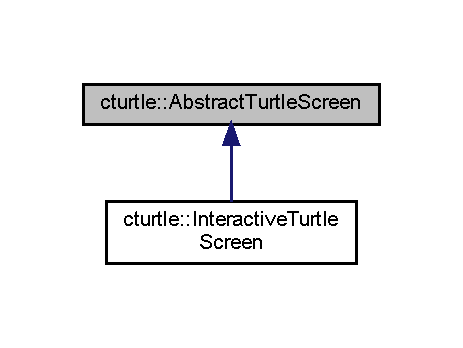
\includegraphics[width=222pt]{classcturtle_1_1AbstractTurtleScreen__inherit__graph}
\end{center}
\end{figure}
\doxysubsection*{Public Member Functions}
\begin{DoxyCompactItemize}
\item 
virtual void \mbox{\hyperlink{classcturtle_1_1AbstractTurtleScreen_ad8e8c7abcc876b2ddd7d19494bb71985}{tracer}} (int countmax, unsigned int delay\+MS=10)=0
\item 
virtual int \mbox{\hyperlink{classcturtle_1_1AbstractTurtleScreen_a1ddb52212ec961b27c9c40c0786a2dee}{window\+\_\+width}} () const =0
\item 
virtual int \mbox{\hyperlink{classcturtle_1_1AbstractTurtleScreen_a8a03d248a0a7b02e88d891f24a27fb8d}{window\+\_\+height}} () const =0
\item 
virtual \mbox{\hyperlink{classcturtle_1_1Color}{Color}} \mbox{\hyperlink{classcturtle_1_1AbstractTurtleScreen_ac542d5c180390842d99a6078965aa077}{bgcolor}} () const =0
\item 
virtual void \mbox{\hyperlink{classcturtle_1_1AbstractTurtleScreen_ac421f2018c0f88e3bc3b36f716c3fc04}{bgcolor}} (const \mbox{\hyperlink{classcturtle_1_1Color}{Color}} \&c)=0
\item 
virtual void \mbox{\hyperlink{classcturtle_1_1AbstractTurtleScreen_a66a3002d3a6713e615a58b345ec21062}{mode}} (Screen\+Mode mode)=0
\item 
virtual Screen\+Mode \mbox{\hyperlink{classcturtle_1_1AbstractTurtleScreen_a6f4031d934f2785165b382384611b19d}{mode}} () const =0
\item 
virtual void \mbox{\hyperlink{classcturtle_1_1AbstractTurtleScreen_ad37d1976302819c74e766290a2128072}{clearscreen}} ()=0
\item 
void \mbox{\hyperlink{classcturtle_1_1AbstractTurtleScreen_abae240a2ba949c1628bb01ad850fb32b}{clear}} ()
\item 
virtual void \mbox{\hyperlink{classcturtle_1_1AbstractTurtleScreen_a2a705428bc1fd07300ebcf1a6b10e989}{resetscreen}} ()=0
\item 
void \mbox{\hyperlink{classcturtle_1_1AbstractTurtleScreen_ac791e1eca792e71c356006c96eb98788}{reset}} ()
\item 
virtual bool \mbox{\hyperlink{classcturtle_1_1AbstractTurtleScreen_aa9651fa98eefdb83fd99d476217b5414}{supports\+\_\+live\+\_\+animation}} () const =0
\item 
\mbox{\Hypertarget{classcturtle_1_1AbstractTurtleScreen_a67b23a8833900072eb9079b836b1796e}\label{classcturtle_1_1AbstractTurtleScreen_a67b23a8833900072eb9079b836b1796e}} 
virtual \mbox{\hyperlink{structcturtle_1_1ivec2}{ivec2}} {\bfseries screensize} (\mbox{\hyperlink{classcturtle_1_1Color}{Color}} \&bg)=0
\item 
\mbox{\Hypertarget{classcturtle_1_1AbstractTurtleScreen_a9e8443b41b8d0765993b1b6fb5cfb94f}\label{classcturtle_1_1AbstractTurtleScreen_a9e8443b41b8d0765993b1b6fb5cfb94f}} 
virtual \mbox{\hyperlink{structcturtle_1_1ivec2}{ivec2}} {\bfseries screensize} ()=0
\item 
\mbox{\Hypertarget{classcturtle_1_1AbstractTurtleScreen_a85ab4fad60333c90051219e32a299686}\label{classcturtle_1_1AbstractTurtleScreen_a85ab4fad60333c90051219e32a299686}} 
virtual void {\bfseries update} (bool invalidate\+Draw=false, bool process\+Input=true)=0
\item 
\mbox{\Hypertarget{classcturtle_1_1AbstractTurtleScreen_a779ca47025b1d005ab0dcc5a0c368ac8}\label{classcturtle_1_1AbstractTurtleScreen_a779ca47025b1d005ab0dcc5a0c368ac8}} 
virtual void {\bfseries delay} (unsigned int ms)=0
\item 
\mbox{\Hypertarget{classcturtle_1_1AbstractTurtleScreen_ab1d6569b39973c6df6507e4f9890407e}\label{classcturtle_1_1AbstractTurtleScreen_ab1d6569b39973c6df6507e4f9890407e}} 
virtual unsigned int {\bfseries delay} ()=0
\item 
virtual void \mbox{\hyperlink{classcturtle_1_1AbstractTurtleScreen_a04de9abc6c3a8f046568c7d1a842d168}{bye}} ()=0
\item 
\mbox{\Hypertarget{classcturtle_1_1AbstractTurtleScreen_a090a77eb87eab4a3d3e4f1b9476abff2}\label{classcturtle_1_1AbstractTurtleScreen_a090a77eb87eab4a3d3e4f1b9476abff2}} 
virtual Image \& {\bfseries getcanvas} ()=0
\item 
\mbox{\Hypertarget{classcturtle_1_1AbstractTurtleScreen_a5a68db439eb8e5016a290529d62610f5}\label{classcturtle_1_1AbstractTurtleScreen_a5a68db439eb8e5016a290529d62610f5}} 
virtual bool {\bfseries isclosed} ()=0
\item 
\mbox{\Hypertarget{classcturtle_1_1AbstractTurtleScreen_a6bf8b7618ccd22087cc4fcb95d9e2ac5}\label{classcturtle_1_1AbstractTurtleScreen_a6bf8b7618ccd22087cc4fcb95d9e2ac5}} 
virtual void {\bfseries redraw} (bool invalidate=false)=0
\item 
\mbox{\Hypertarget{classcturtle_1_1AbstractTurtleScreen_a602b6058a1d56e27700155987b791056}\label{classcturtle_1_1AbstractTurtleScreen_a602b6058a1d56e27700155987b791056}} 
virtual \mbox{\hyperlink{classcturtle_1_1Transform}{Transform}} \mbox{\hyperlink{classcturtle_1_1AbstractTurtleScreen_a602b6058a1d56e27700155987b791056}{screentransform}} () const =0
\begin{DoxyCompactList}\small\item\em Calculates and returns the root-\/level screen transformation. \end{DoxyCompactList}\item 
\mbox{\Hypertarget{classcturtle_1_1AbstractTurtleScreen_aa82ae80751e1f6f71b07d2c0ba72e5e8}\label{classcturtle_1_1AbstractTurtleScreen_aa82ae80751e1f6f71b07d2c0ba72e5e8}} 
virtual void \mbox{\hyperlink{classcturtle_1_1AbstractTurtleScreen_aa82ae80751e1f6f71b07d2c0ba72e5e8}{add}} (\mbox{\hyperlink{classcturtle_1_1Turtle}{Turtle}} \&turtle)=0
\begin{DoxyCompactList}\small\item\em Adds the specified turtle to this screen. The turtle cannot belong to other screens, as that would break ownership responsibility. \end{DoxyCompactList}\item 
virtual std\+::list$<$ \mbox{\hyperlink{structcturtle_1_1SceneObject}{Scene\+Object}} $>$ \& \mbox{\hyperlink{classcturtle_1_1AbstractTurtleScreen_ab4524119329c3ab3ce2a9a864ec87437}{get\+Scene}} ()=0
\begin{DoxyCompactList}\small\item\em Returns a read-\/write reference to the list of scene objects currently residing on this screen. \end{DoxyCompactList}\item 
virtual \mbox{\hyperlink{classcturtle_1_1AbstractDrawableObject}{Abstract\+Drawable\+Object}} \& \mbox{\hyperlink{classcturtle_1_1AbstractTurtleScreen_a63ad1c2ec491e0a8773fc53aac0b9c3a}{shape}} (const std\+::string \&name)=0
\begin{DoxyCompactList}\small\item\em Returns a read-\/write reference to the registered shape with the specified name. \end{DoxyCompactList}\item 
virtual const \mbox{\hyperlink{classcturtle_1_1BitmapFont}{Bitmap\+Font}} \& \mbox{\hyperlink{classcturtle_1_1AbstractTurtleScreen_a353979f88702d7be0a5476f47f3be254}{font}} (const std\+::string \&name) const =0
\begin{DoxyCompactList}\small\item\em Returns a read-\/only reference to a previously loaded bitmap font. \end{DoxyCompactList}\end{DoxyCompactItemize}
\doxysubsection*{Protected Member Functions}
\begin{DoxyCompactItemize}
\item 
Image \mbox{\hyperlink{classcturtle_1_1AbstractTurtleScreen_aa8a517a5311e0eb1fbb32ab8b1376a9d}{decode\+Default\+Font}} () const
\end{DoxyCompactItemize}
\doxysubsection*{Protected Attributes}
\begin{DoxyCompactItemize}
\item 
std\+::unordered\+\_\+map$<$ std\+::string, \mbox{\hyperlink{classcturtle_1_1Polygon}{Polygon}} $>$ {\bfseries shapes}
\end{DoxyCompactItemize}


\doxysubsection{Detailed Description}
The \mbox{\hyperlink{classcturtle_1_1AbstractTurtleScreen}{Abstract\+Turtle\+Screen}} class is the abstract type for most turtle functionality. It intentionally excludes all input/output functionality, allowing for two intended derivates\+: an \char`\"{}interactive\char`\"{} screen, vs an \char`\"{}offline rendering\char`\"{} screen. The \mbox{\hyperlink{classcturtle_1_1Turtle}{Turtle}} class doesn\textquotesingle{}t care which one it gets attached to. 

\doxysubsection{Member Function Documentation}
\mbox{\Hypertarget{classcturtle_1_1AbstractTurtleScreen_ac542d5c180390842d99a6078965aa077}\label{classcturtle_1_1AbstractTurtleScreen_ac542d5c180390842d99a6078965aa077}} 
\index{cturtle::AbstractTurtleScreen@{cturtle::AbstractTurtleScreen}!bgcolor@{bgcolor}}
\index{bgcolor@{bgcolor}!cturtle::AbstractTurtleScreen@{cturtle::AbstractTurtleScreen}}
\doxysubsubsection{\texorpdfstring{bgcolor()}{bgcolor()}\hspace{0.1cm}{\footnotesize\ttfamily [1/2]}}
{\footnotesize\ttfamily virtual \mbox{\hyperlink{classcturtle_1_1Color}{Color}} cturtle\+::\+Abstract\+Turtle\+Screen\+::bgcolor (\begin{DoxyParamCaption}{ }\end{DoxyParamCaption}) const\hspace{0.3cm}{\ttfamily [pure virtual]}}

Returns the current background color. 

Implemented in \mbox{\hyperlink{classcturtle_1_1InteractiveTurtleScreen_a55289593218ba99904f7957700ef7dae}{cturtle\+::\+Interactive\+Turtle\+Screen}}.

\mbox{\Hypertarget{classcturtle_1_1AbstractTurtleScreen_ac421f2018c0f88e3bc3b36f716c3fc04}\label{classcturtle_1_1AbstractTurtleScreen_ac421f2018c0f88e3bc3b36f716c3fc04}} 
\index{cturtle::AbstractTurtleScreen@{cturtle::AbstractTurtleScreen}!bgcolor@{bgcolor}}
\index{bgcolor@{bgcolor}!cturtle::AbstractTurtleScreen@{cturtle::AbstractTurtleScreen}}
\doxysubsubsection{\texorpdfstring{bgcolor()}{bgcolor()}\hspace{0.1cm}{\footnotesize\ttfamily [2/2]}}
{\footnotesize\ttfamily virtual void cturtle\+::\+Abstract\+Turtle\+Screen\+::bgcolor (\begin{DoxyParamCaption}\item[{const \mbox{\hyperlink{classcturtle_1_1Color}{Color}} \&}]{c }\end{DoxyParamCaption})\hspace{0.3cm}{\ttfamily [pure virtual]}}

Sets the current background color. 

Implemented in \mbox{\hyperlink{classcturtle_1_1InteractiveTurtleScreen_acb5441704b45a01830d69df46a23732f}{cturtle\+::\+Interactive\+Turtle\+Screen}}.

\mbox{\Hypertarget{classcturtle_1_1AbstractTurtleScreen_a04de9abc6c3a8f046568c7d1a842d168}\label{classcturtle_1_1AbstractTurtleScreen_a04de9abc6c3a8f046568c7d1a842d168}} 
\index{cturtle::AbstractTurtleScreen@{cturtle::AbstractTurtleScreen}!bye@{bye}}
\index{bye@{bye}!cturtle::AbstractTurtleScreen@{cturtle::AbstractTurtleScreen}}
\doxysubsubsection{\texorpdfstring{bye()}{bye()}}
{\footnotesize\ttfamily virtual void cturtle\+::\+Abstract\+Turtle\+Screen\+::bye (\begin{DoxyParamCaption}{ }\end{DoxyParamCaption})\hspace{0.3cm}{\ttfamily [pure virtual]}}

Closes this turtle screen. 

Implemented in \mbox{\hyperlink{classcturtle_1_1InteractiveTurtleScreen_a045b2cc0c8869140015abcc11226a714}{cturtle\+::\+Interactive\+Turtle\+Screen}}.

\mbox{\Hypertarget{classcturtle_1_1AbstractTurtleScreen_abae240a2ba949c1628bb01ad850fb32b}\label{classcturtle_1_1AbstractTurtleScreen_abae240a2ba949c1628bb01ad850fb32b}} 
\index{cturtle::AbstractTurtleScreen@{cturtle::AbstractTurtleScreen}!clear@{clear}}
\index{clear@{clear}!cturtle::AbstractTurtleScreen@{cturtle::AbstractTurtleScreen}}
\doxysubsubsection{\texorpdfstring{clear()}{clear()}}
{\footnotesize\ttfamily void cturtle\+::\+Abstract\+Turtle\+Screen\+::clear (\begin{DoxyParamCaption}{ }\end{DoxyParamCaption})\hspace{0.3cm}{\ttfamily [inline]}}

Alias for clearscreen function \begin{DoxySeeAlso}{See also}
\mbox{\hyperlink{classcturtle_1_1AbstractTurtleScreen_ad37d1976302819c74e766290a2128072}{clearscreen()}} 
\end{DoxySeeAlso}
\mbox{\Hypertarget{classcturtle_1_1AbstractTurtleScreen_ad37d1976302819c74e766290a2128072}\label{classcturtle_1_1AbstractTurtleScreen_ad37d1976302819c74e766290a2128072}} 
\index{cturtle::AbstractTurtleScreen@{cturtle::AbstractTurtleScreen}!clearscreen@{clearscreen}}
\index{clearscreen@{clearscreen}!cturtle::AbstractTurtleScreen@{cturtle::AbstractTurtleScreen}}
\doxysubsubsection{\texorpdfstring{clearscreen()}{clearscreen()}}
{\footnotesize\ttfamily virtual void cturtle\+::\+Abstract\+Turtle\+Screen\+::clearscreen (\begin{DoxyParamCaption}{ }\end{DoxyParamCaption})\hspace{0.3cm}{\ttfamily [pure virtual]}}

Clears the screen. 

Implemented in \mbox{\hyperlink{classcturtle_1_1InteractiveTurtleScreen_ae4e184867d7ed83c58e0ef9e730f4d73}{cturtle\+::\+Interactive\+Turtle\+Screen}}.

\mbox{\Hypertarget{classcturtle_1_1AbstractTurtleScreen_aa8a517a5311e0eb1fbb32ab8b1376a9d}\label{classcturtle_1_1AbstractTurtleScreen_aa8a517a5311e0eb1fbb32ab8b1376a9d}} 
\index{cturtle::AbstractTurtleScreen@{cturtle::AbstractTurtleScreen}!decodeDefaultFont@{decodeDefaultFont}}
\index{decodeDefaultFont@{decodeDefaultFont}!cturtle::AbstractTurtleScreen@{cturtle::AbstractTurtleScreen}}
\doxysubsubsection{\texorpdfstring{decodeDefaultFont()}{decodeDefaultFont()}}
{\footnotesize\ttfamily Image cturtle\+::\+Abstract\+Turtle\+Screen\+::decode\+Default\+Font (\begin{DoxyParamCaption}{ }\end{DoxyParamCaption}) const\hspace{0.3cm}{\ttfamily [inline]}, {\ttfamily [protected]}}

Decodes the default font image from memory. The font is encoded as 1 bit per pixel (on/off) for simplicity, and is relatively easily decoded through bit-\/shifting.

The loading of this was delegated to the \mbox{\hyperlink{classcturtle_1_1AbstractTurtleScreen}{Abstract\+Turtle\+Screen}} class simply because all derived classes should have an idea of their own internal states, however they will A\+LL have these managed states, and thus A\+LL derived classes will need to call this function at some point while performing default initialization. \begin{DoxyReturn}{Returns}
the decoded default font image. 
\end{DoxyReturn}
\mbox{\Hypertarget{classcturtle_1_1AbstractTurtleScreen_a353979f88702d7be0a5476f47f3be254}\label{classcturtle_1_1AbstractTurtleScreen_a353979f88702d7be0a5476f47f3be254}} 
\index{cturtle::AbstractTurtleScreen@{cturtle::AbstractTurtleScreen}!font@{font}}
\index{font@{font}!cturtle::AbstractTurtleScreen@{cturtle::AbstractTurtleScreen}}
\doxysubsubsection{\texorpdfstring{font()}{font()}}
{\footnotesize\ttfamily virtual const \mbox{\hyperlink{classcturtle_1_1BitmapFont}{Bitmap\+Font}}\& cturtle\+::\+Abstract\+Turtle\+Screen\+::font (\begin{DoxyParamCaption}\item[{const std\+::string \&}]{name }\end{DoxyParamCaption}) const\hspace{0.3cm}{\ttfamily [pure virtual]}}



Returns a read-\/only reference to a previously loaded bitmap font. 

\begin{DoxyReturn}{Returns}
a previously loaded font by its specified name. 
\end{DoxyReturn}


Implemented in \mbox{\hyperlink{classcturtle_1_1InteractiveTurtleScreen_a501149617310118e21df8f527580339e}{cturtle\+::\+Interactive\+Turtle\+Screen}}.

\mbox{\Hypertarget{classcturtle_1_1AbstractTurtleScreen_ab4524119329c3ab3ce2a9a864ec87437}\label{classcturtle_1_1AbstractTurtleScreen_ab4524119329c3ab3ce2a9a864ec87437}} 
\index{cturtle::AbstractTurtleScreen@{cturtle::AbstractTurtleScreen}!getScene@{getScene}}
\index{getScene@{getScene}!cturtle::AbstractTurtleScreen@{cturtle::AbstractTurtleScreen}}
\doxysubsubsection{\texorpdfstring{getScene()}{getScene()}}
{\footnotesize\ttfamily virtual std\+::list$<$\mbox{\hyperlink{structcturtle_1_1SceneObject}{Scene\+Object}}$>$\& cturtle\+::\+Abstract\+Turtle\+Screen\+::get\+Scene (\begin{DoxyParamCaption}{ }\end{DoxyParamCaption})\hspace{0.3cm}{\ttfamily [pure virtual]}}



Returns a read-\/write reference to the list of scene objects currently residing on this screen. 

\begin{DoxyReturn}{Returns}
the list of scene objects currently residing on this screen. 
\end{DoxyReturn}


Implemented in \mbox{\hyperlink{classcturtle_1_1InteractiveTurtleScreen_aa1bd826458a718e7605424d5767f79c9}{cturtle\+::\+Interactive\+Turtle\+Screen}}.

\mbox{\Hypertarget{classcturtle_1_1AbstractTurtleScreen_a6f4031d934f2785165b382384611b19d}\label{classcturtle_1_1AbstractTurtleScreen_a6f4031d934f2785165b382384611b19d}} 
\index{cturtle::AbstractTurtleScreen@{cturtle::AbstractTurtleScreen}!mode@{mode}}
\index{mode@{mode}!cturtle::AbstractTurtleScreen@{cturtle::AbstractTurtleScreen}}
\doxysubsubsection{\texorpdfstring{mode()}{mode()}\hspace{0.1cm}{\footnotesize\ttfamily [1/2]}}
{\footnotesize\ttfamily virtual Screen\+Mode cturtle\+::\+Abstract\+Turtle\+Screen\+::mode (\begin{DoxyParamCaption}{ }\end{DoxyParamCaption}) const\hspace{0.3cm}{\ttfamily [pure virtual]}}

Returns the current screen mode. 

Implemented in \mbox{\hyperlink{classcturtle_1_1InteractiveTurtleScreen_af65c66dbfe93fa748944f7a6d299080e}{cturtle\+::\+Interactive\+Turtle\+Screen}}.

\mbox{\Hypertarget{classcturtle_1_1AbstractTurtleScreen_a66a3002d3a6713e615a58b345ec21062}\label{classcturtle_1_1AbstractTurtleScreen_a66a3002d3a6713e615a58b345ec21062}} 
\index{cturtle::AbstractTurtleScreen@{cturtle::AbstractTurtleScreen}!mode@{mode}}
\index{mode@{mode}!cturtle::AbstractTurtleScreen@{cturtle::AbstractTurtleScreen}}
\doxysubsubsection{\texorpdfstring{mode()}{mode()}\hspace{0.1cm}{\footnotesize\ttfamily [2/2]}}
{\footnotesize\ttfamily virtual void cturtle\+::\+Abstract\+Turtle\+Screen\+::mode (\begin{DoxyParamCaption}\item[{Screen\+Mode}]{mode }\end{DoxyParamCaption})\hspace{0.3cm}{\ttfamily [pure virtual]}}

Sets the current screen mode. 

Implemented in \mbox{\hyperlink{classcturtle_1_1InteractiveTurtleScreen_a1c666afe65211cf9eedaffa17206a697}{cturtle\+::\+Interactive\+Turtle\+Screen}}.

\mbox{\Hypertarget{classcturtle_1_1AbstractTurtleScreen_ac791e1eca792e71c356006c96eb98788}\label{classcturtle_1_1AbstractTurtleScreen_ac791e1eca792e71c356006c96eb98788}} 
\index{cturtle::AbstractTurtleScreen@{cturtle::AbstractTurtleScreen}!reset@{reset}}
\index{reset@{reset}!cturtle::AbstractTurtleScreen@{cturtle::AbstractTurtleScreen}}
\doxysubsubsection{\texorpdfstring{reset()}{reset()}}
{\footnotesize\ttfamily void cturtle\+::\+Abstract\+Turtle\+Screen\+::reset (\begin{DoxyParamCaption}{ }\end{DoxyParamCaption})\hspace{0.3cm}{\ttfamily [inline]}}

Resets all turtles belonging to this screen to their original state. \mbox{\Hypertarget{classcturtle_1_1AbstractTurtleScreen_a2a705428bc1fd07300ebcf1a6b10e989}\label{classcturtle_1_1AbstractTurtleScreen_a2a705428bc1fd07300ebcf1a6b10e989}} 
\index{cturtle::AbstractTurtleScreen@{cturtle::AbstractTurtleScreen}!resetscreen@{resetscreen}}
\index{resetscreen@{resetscreen}!cturtle::AbstractTurtleScreen@{cturtle::AbstractTurtleScreen}}
\doxysubsubsection{\texorpdfstring{resetscreen()}{resetscreen()}}
{\footnotesize\ttfamily virtual void cturtle\+::\+Abstract\+Turtle\+Screen\+::resetscreen (\begin{DoxyParamCaption}{ }\end{DoxyParamCaption})\hspace{0.3cm}{\ttfamily [pure virtual]}}

Resets all turtles belonging to this screen to their original state. 

Implemented in \mbox{\hyperlink{classcturtle_1_1InteractiveTurtleScreen_a06471bf6c8c02768fb0acd89649c72c2}{cturtle\+::\+Interactive\+Turtle\+Screen}}.

\mbox{\Hypertarget{classcturtle_1_1AbstractTurtleScreen_a63ad1c2ec491e0a8773fc53aac0b9c3a}\label{classcturtle_1_1AbstractTurtleScreen_a63ad1c2ec491e0a8773fc53aac0b9c3a}} 
\index{cturtle::AbstractTurtleScreen@{cturtle::AbstractTurtleScreen}!shape@{shape}}
\index{shape@{shape}!cturtle::AbstractTurtleScreen@{cturtle::AbstractTurtleScreen}}
\doxysubsubsection{\texorpdfstring{shape()}{shape()}}
{\footnotesize\ttfamily virtual \mbox{\hyperlink{classcturtle_1_1AbstractDrawableObject}{Abstract\+Drawable\+Object}}\& cturtle\+::\+Abstract\+Turtle\+Screen\+::shape (\begin{DoxyParamCaption}\item[{const std\+::string \&}]{name }\end{DoxyParamCaption})\hspace{0.3cm}{\ttfamily [pure virtual]}}



Returns a read-\/write reference to the registered shape with the specified name. 


\begin{DoxyParams}{Parameters}
{\em name} & of the shape \\
\hline
\end{DoxyParams}
\begin{DoxyReturn}{Returns}
read-\/write reference to the associated shape 
\end{DoxyReturn}


Implemented in \mbox{\hyperlink{classcturtle_1_1InteractiveTurtleScreen_ae855fb3d2acd831ce751e9387b8edc06}{cturtle\+::\+Interactive\+Turtle\+Screen}}.

\mbox{\Hypertarget{classcturtle_1_1AbstractTurtleScreen_aa9651fa98eefdb83fd99d476217b5414}\label{classcturtle_1_1AbstractTurtleScreen_aa9651fa98eefdb83fd99d476217b5414}} 
\index{cturtle::AbstractTurtleScreen@{cturtle::AbstractTurtleScreen}!supports\_live\_animation@{supports\_live\_animation}}
\index{supports\_live\_animation@{supports\_live\_animation}!cturtle::AbstractTurtleScreen@{cturtle::AbstractTurtleScreen}}
\doxysubsubsection{\texorpdfstring{supports\_live\_animation()}{supports\_live\_animation()}}
{\footnotesize\ttfamily virtual bool cturtle\+::\+Abstract\+Turtle\+Screen\+::supports\+\_\+live\+\_\+animation (\begin{DoxyParamCaption}{ }\end{DoxyParamCaption}) const\hspace{0.3cm}{\ttfamily [pure virtual]}}

\begin{DoxyReturn}{Returns}
a boolean indicating if this turtle screen supports live animation. \char`\"{}\+Live animation\char`\"{} is regarded as the frames of animation that encompass movement over space. 
\end{DoxyReturn}


Implemented in \mbox{\hyperlink{classcturtle_1_1InteractiveTurtleScreen_ad28f7c6e4058541a2c4258b4455fad74}{cturtle\+::\+Interactive\+Turtle\+Screen}}.

\mbox{\Hypertarget{classcturtle_1_1AbstractTurtleScreen_ad8e8c7abcc876b2ddd7d19494bb71985}\label{classcturtle_1_1AbstractTurtleScreen_ad8e8c7abcc876b2ddd7d19494bb71985}} 
\index{cturtle::AbstractTurtleScreen@{cturtle::AbstractTurtleScreen}!tracer@{tracer}}
\index{tracer@{tracer}!cturtle::AbstractTurtleScreen@{cturtle::AbstractTurtleScreen}}
\doxysubsubsection{\texorpdfstring{tracer()}{tracer()}}
{\footnotesize\ttfamily virtual void cturtle\+::\+Abstract\+Turtle\+Screen\+::tracer (\begin{DoxyParamCaption}\item[{int}]{countmax,  }\item[{unsigned int}]{delay\+MS = {\ttfamily 10} }\end{DoxyParamCaption})\hspace{0.3cm}{\ttfamily [pure virtual]}}

Sets the tracer setting for this window. 

Implemented in \mbox{\hyperlink{classcturtle_1_1InteractiveTurtleScreen_ac6cbbcf714c490abb300cd6a931950f3}{cturtle\+::\+Interactive\+Turtle\+Screen}}.

\mbox{\Hypertarget{classcturtle_1_1AbstractTurtleScreen_a8a03d248a0a7b02e88d891f24a27fb8d}\label{classcturtle_1_1AbstractTurtleScreen_a8a03d248a0a7b02e88d891f24a27fb8d}} 
\index{cturtle::AbstractTurtleScreen@{cturtle::AbstractTurtleScreen}!window\_height@{window\_height}}
\index{window\_height@{window\_height}!cturtle::AbstractTurtleScreen@{cturtle::AbstractTurtleScreen}}
\doxysubsubsection{\texorpdfstring{window\_height()}{window\_height()}}
{\footnotesize\ttfamily virtual int cturtle\+::\+Abstract\+Turtle\+Screen\+::window\+\_\+height (\begin{DoxyParamCaption}{ }\end{DoxyParamCaption}) const\hspace{0.3cm}{\ttfamily [pure virtual]}}

Returns the height of the window, in pixels. 

Implemented in \mbox{\hyperlink{classcturtle_1_1InteractiveTurtleScreen_a259883332b284e3b8a97b5bfb74f988d}{cturtle\+::\+Interactive\+Turtle\+Screen}}.

\mbox{\Hypertarget{classcturtle_1_1AbstractTurtleScreen_a1ddb52212ec961b27c9c40c0786a2dee}\label{classcturtle_1_1AbstractTurtleScreen_a1ddb52212ec961b27c9c40c0786a2dee}} 
\index{cturtle::AbstractTurtleScreen@{cturtle::AbstractTurtleScreen}!window\_width@{window\_width}}
\index{window\_width@{window\_width}!cturtle::AbstractTurtleScreen@{cturtle::AbstractTurtleScreen}}
\doxysubsubsection{\texorpdfstring{window\_width()}{window\_width()}}
{\footnotesize\ttfamily virtual int cturtle\+::\+Abstract\+Turtle\+Screen\+::window\+\_\+width (\begin{DoxyParamCaption}{ }\end{DoxyParamCaption}) const\hspace{0.3cm}{\ttfamily [pure virtual]}}

Returns the width of the window, in pixels. 

Implemented in \mbox{\hyperlink{classcturtle_1_1InteractiveTurtleScreen_aefeb4e90fae07d043677f3dee9a29026}{cturtle\+::\+Interactive\+Turtle\+Screen}}.



\doxysubsection{Member Data Documentation}
\mbox{\Hypertarget{classcturtle_1_1AbstractTurtleScreen_a3ccd6578530b23b43b60884777c99603}\label{classcturtle_1_1AbstractTurtleScreen_a3ccd6578530b23b43b60884777c99603}} 
\index{cturtle::AbstractTurtleScreen@{cturtle::AbstractTurtleScreen}!shapes@{shapes}}
\index{shapes@{shapes}!cturtle::AbstractTurtleScreen@{cturtle::AbstractTurtleScreen}}
\doxysubsubsection{\texorpdfstring{shapes}{shapes}}
{\footnotesize\ttfamily std\+::unordered\+\_\+map$<$std\+::string, \mbox{\hyperlink{classcturtle_1_1Polygon}{Polygon}}$>$ cturtle\+::\+Abstract\+Turtle\+Screen\+::shapes\hspace{0.3cm}{\ttfamily [protected]}}

{\bfseries Initial value\+:}
\begin{DoxyCode}{0}
\DoxyCodeLine{= \{}
\DoxyCodeLine{                }
\DoxyCodeLine{                \{\textcolor{stringliteral}{"triangle"},}
\DoxyCodeLine{                        Polygon\{}
\DoxyCodeLine{                                \{0, 0\},}
\DoxyCodeLine{                                \{-\/5, 5\},}
\DoxyCodeLine{                                \{5, 5\}\}\},}
\DoxyCodeLine{                \{\textcolor{stringliteral}{"square"},}
\DoxyCodeLine{                        Polygon\{}
\DoxyCodeLine{                                \{-\/5, -\/5\},}
\DoxyCodeLine{                                \{-\/5, 5\},}
\DoxyCodeLine{                                \{5, 5\},}
\DoxyCodeLine{                                \{5, -\/5\}\}\},}
\DoxyCodeLine{                \{\textcolor{stringliteral}{"indented triangle"},}
\DoxyCodeLine{                        Polygon\{}
\DoxyCodeLine{                                }
\DoxyCodeLine{                                \{0, 0\},}
\DoxyCodeLine{                                \{-\/5, 10\},}
\DoxyCodeLine{                                \{0, 8\},}
\DoxyCodeLine{                                \{5, 10\}\}\},}
\DoxyCodeLine{                \{\textcolor{stringliteral}{"arrow"},}
\DoxyCodeLine{                        Polygon\{}
\DoxyCodeLine{                                \{0, 0\},}
\DoxyCodeLine{                                \{-\/5, 5\},}
\DoxyCodeLine{                                \{-\/3, 5\},}
\DoxyCodeLine{                                \{-\/3, 10\},}
\DoxyCodeLine{                                \{3, 10\},}
\DoxyCodeLine{                                \{3, 5\},}
\DoxyCodeLine{                                \{5, 5\}\}\}}
\DoxyCodeLine{        \}}

\end{DoxyCode}


The documentation for this class was generated from the following file\+:\begin{DoxyCompactItemize}
\item 
C\+Turtle.\+hpp\end{DoxyCompactItemize}

\hypertarget{classcturtle_1_1Circle}{}\doxysection{cturtle\+::Circle Class Reference}
\label{classcturtle_1_1Circle}\index{cturtle::Circle@{cturtle::Circle}}


The \mbox{\hyperlink{classcturtle_1_1Circle}{Circle}} class holds a radius and total number of steps, used to generate and draw a circles geometry.  




{\ttfamily \#include $<$CTurtle.\+hpp$>$}



Inheritance diagram for cturtle\+::Circle\+:\nopagebreak
\begin{figure}[H]
\begin{center}
\leavevmode
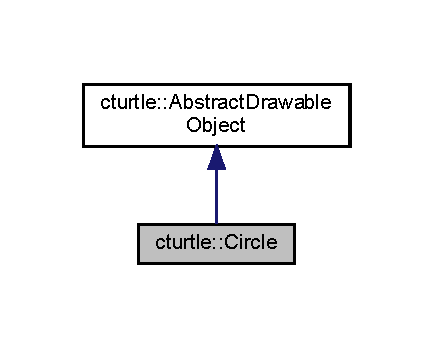
\includegraphics[width=208pt]{classcturtle_1_1Circle__inherit__graph}
\end{center}
\end{figure}


Collaboration diagram for cturtle\+::Circle\+:\nopagebreak
\begin{figure}[H]
\begin{center}
\leavevmode
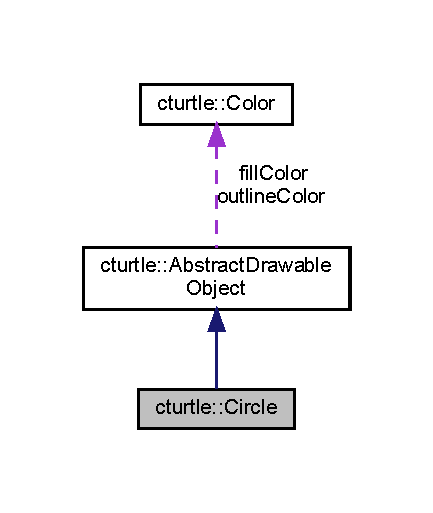
\includegraphics[width=208pt]{classcturtle_1_1Circle__coll__graph}
\end{center}
\end{figure}
\doxysubsection*{Public Member Functions}
\begin{DoxyCompactItemize}
\item 
\mbox{\Hypertarget{classcturtle_1_1Circle_adc2f1cb13db5aa45558541ebb5a6f975}\label{classcturtle_1_1Circle_adc2f1cb13db5aa45558541ebb5a6f975}} 
\mbox{\hyperlink{classcturtle_1_1Circle_adc2f1cb13db5aa45558541ebb5a6f975}{Circle}} ()=default
\begin{DoxyCompactList}\small\item\em Empty constructor. \end{DoxyCompactList}\item 
\mbox{\hyperlink{classcturtle_1_1Circle_a8c63fb9d9b6c0bafa51519bbdf910f2d}{Circle}} (int \mbox{\hyperlink{classcturtle_1_1Circle_a01dfc45c6a56b58e040e4de2cc8abda5}{radius}}, int \mbox{\hyperlink{classcturtle_1_1Circle_a5bf905891d9a0d21b08070698c71321e}{steps}}, const \mbox{\hyperlink{classcturtle_1_1Color}{Color}} \&\mbox{\hyperlink{classcturtle_1_1AbstractDrawableObject_a37d635a02ad3e5206a6eb99b7b5f1963}{fill\+Color}}, int \mbox{\hyperlink{classcturtle_1_1AbstractDrawableObject_aeffaecc245057e9a42e5688671a77f52}{outline\+Width}}=0, const \mbox{\hyperlink{classcturtle_1_1Color}{Color}} \&\mbox{\hyperlink{classcturtle_1_1AbstractDrawableObject_abd04640855e7623bb84b52babd8b32b6}{outline\+Color}}=\mbox{\hyperlink{classcturtle_1_1Color}{Color}}())
\begin{DoxyCompactList}\small\item\em Radius and step assignment constructor. \end{DoxyCompactList}\item 
\mbox{\hyperlink{classcturtle_1_1Circle_a07e85dc7f96facbfa3c2e2791209e7e9}{Circle}} (const \mbox{\hyperlink{classcturtle_1_1Circle}{Circle}} \&other)=default
\begin{DoxyCompactList}\small\item\em Copy constructor. \end{DoxyCompactList}\item 
\mbox{\Hypertarget{classcturtle_1_1Circle_ae6ba7c80556d4073fb3a223d38d24108}\label{classcturtle_1_1Circle_ae6ba7c80556d4073fb3a223d38d24108}} 
\mbox{\hyperlink{classcturtle_1_1AbstractDrawableObject}{Abstract\+Drawable\+Object}} $\ast$ \mbox{\hyperlink{classcturtle_1_1Circle_ae6ba7c80556d4073fb3a223d38d24108}{copy}} () const override
\begin{DoxyCompactList}\small\item\em Returns a pointer to a copy of this drawable object, allocated with NEW. Result must be deleted at the responsibility of the invoker. \end{DoxyCompactList}\item 
void \mbox{\hyperlink{classcturtle_1_1Circle_ace43ef3ce3c151a340d269546722d05e}{draw}} (const \mbox{\hyperlink{classcturtle_1_1Transform}{Transform}} \&t, Image \&img\+Ref) const override
\begin{DoxyCompactList}\small\item\em This function is intended to draw all applicable geometry in this object to the specified image, with the specified transform, with the specified color. This function is intended to be overloaded by child classes to draw applicable geometry to an image, acting as a canvas. \end{DoxyCompactList}\end{DoxyCompactItemize}
\doxysubsection*{Public Attributes}
\begin{DoxyCompactItemize}
\item 
int \mbox{\hyperlink{classcturtle_1_1Circle_a01dfc45c6a56b58e040e4de2cc8abda5}{radius}} = 10
\item 
int \mbox{\hyperlink{classcturtle_1_1Circle_a5bf905891d9a0d21b08070698c71321e}{steps}} = 10
\end{DoxyCompactItemize}
\doxysubsection*{Additional Inherited Members}


\doxysubsection{Detailed Description}
The \mbox{\hyperlink{classcturtle_1_1Circle}{Circle}} class holds a radius and total number of steps, used to generate and draw a circles geometry. 

\doxysubsection{Constructor \& Destructor Documentation}
\mbox{\Hypertarget{classcturtle_1_1Circle_a8c63fb9d9b6c0bafa51519bbdf910f2d}\label{classcturtle_1_1Circle_a8c63fb9d9b6c0bafa51519bbdf910f2d}} 
\index{cturtle::Circle@{cturtle::Circle}!Circle@{Circle}}
\index{Circle@{Circle}!cturtle::Circle@{cturtle::Circle}}
\doxysubsubsection{\texorpdfstring{Circle()}{Circle()}\hspace{0.1cm}{\footnotesize\ttfamily [1/2]}}
{\footnotesize\ttfamily cturtle\+::\+Circle\+::\+Circle (\begin{DoxyParamCaption}\item[{int}]{radius,  }\item[{int}]{steps,  }\item[{const \mbox{\hyperlink{classcturtle_1_1Color}{Color}} \&}]{fill\+Color,  }\item[{int}]{outline\+Width = {\ttfamily 0},  }\item[{const \mbox{\hyperlink{classcturtle_1_1Color}{Color}} \&}]{outline\+Color = {\ttfamily \mbox{\hyperlink{classcturtle_1_1Color}{Color}}()} }\end{DoxyParamCaption})\hspace{0.3cm}{\ttfamily [inline]}}



Radius and step assignment constructor. 


\begin{DoxyParams}{Parameters}
{\em radius} & The radius, in pixels, of this circle. \\
\hline
{\em steps} & The number of vertices used by this circle. \\
\hline
\end{DoxyParams}
\mbox{\Hypertarget{classcturtle_1_1Circle_a07e85dc7f96facbfa3c2e2791209e7e9}\label{classcturtle_1_1Circle_a07e85dc7f96facbfa3c2e2791209e7e9}} 
\index{cturtle::Circle@{cturtle::Circle}!Circle@{Circle}}
\index{Circle@{Circle}!cturtle::Circle@{cturtle::Circle}}
\doxysubsubsection{\texorpdfstring{Circle()}{Circle()}\hspace{0.1cm}{\footnotesize\ttfamily [2/2]}}
{\footnotesize\ttfamily cturtle\+::\+Circle\+::\+Circle (\begin{DoxyParamCaption}\item[{const \mbox{\hyperlink{classcturtle_1_1Circle}{Circle}} \&}]{other }\end{DoxyParamCaption})\hspace{0.3cm}{\ttfamily [default]}}



Copy constructor. 


\begin{DoxyParams}{Parameters}
{\em other} & Another instance of a circle from which to derive value. \\
\hline
\end{DoxyParams}


\doxysubsection{Member Function Documentation}
\mbox{\Hypertarget{classcturtle_1_1Circle_ace43ef3ce3c151a340d269546722d05e}\label{classcturtle_1_1Circle_ace43ef3ce3c151a340d269546722d05e}} 
\index{cturtle::Circle@{cturtle::Circle}!draw@{draw}}
\index{draw@{draw}!cturtle::Circle@{cturtle::Circle}}
\doxysubsubsection{\texorpdfstring{draw()}{draw()}}
{\footnotesize\ttfamily void cturtle\+::\+Circle\+::draw (\begin{DoxyParamCaption}\item[{const \mbox{\hyperlink{classcturtle_1_1Transform}{Transform}} \&}]{t,  }\item[{Image \&}]{img\+Ref }\end{DoxyParamCaption}) const\hspace{0.3cm}{\ttfamily [inline]}, {\ttfamily [override]}, {\ttfamily [virtual]}}



This function is intended to draw all applicable geometry in this object to the specified image, with the specified transform, with the specified color. This function is intended to be overloaded by child classes to draw applicable geometry to an image, acting as a canvas. 


\begin{DoxyParams}{Parameters}
{\em t} & The transform at which to draw the geometry. \\
\hline
{\em img\+Ref} & The canvas on which to draw. \\
\hline
{\em c} & The color with to draw the geometry. \\
\hline
\end{DoxyParams}


Implements \mbox{\hyperlink{classcturtle_1_1AbstractDrawableObject_a7b1ad1e9743d343e0fe577de3978bdad}{cturtle\+::\+Abstract\+Drawable\+Object}}.



\doxysubsection{Member Data Documentation}
\mbox{\Hypertarget{classcturtle_1_1Circle_a01dfc45c6a56b58e040e4de2cc8abda5}\label{classcturtle_1_1Circle_a01dfc45c6a56b58e040e4de2cc8abda5}} 
\index{cturtle::Circle@{cturtle::Circle}!radius@{radius}}
\index{radius@{radius}!cturtle::Circle@{cturtle::Circle}}
\doxysubsubsection{\texorpdfstring{radius}{radius}}
{\footnotesize\ttfamily int cturtle\+::\+Circle\+::radius = 10}

Radius, in pixels, of the geometry generated in the draw function. \mbox{\Hypertarget{classcturtle_1_1Circle_a5bf905891d9a0d21b08070698c71321e}\label{classcturtle_1_1Circle_a5bf905891d9a0d21b08070698c71321e}} 
\index{cturtle::Circle@{cturtle::Circle}!steps@{steps}}
\index{steps@{steps}!cturtle::Circle@{cturtle::Circle}}
\doxysubsubsection{\texorpdfstring{steps}{steps}}
{\footnotesize\ttfamily int cturtle\+::\+Circle\+::steps = 10}

Total number of steps, or vertices, generated in the draw function. The higher this number is, the more \char`\"{}high-\/quality\char`\"{} it can be considered. 

The documentation for this class was generated from the following file\+:\begin{DoxyCompactItemize}
\item 
CTurtle.\+hpp\end{DoxyCompactItemize}

\hypertarget{classcturtle_1_1Color}{}\section{cturtle\+:\+:Color Class Reference}
\label{classcturtle_1_1Color}\index{cturtle\+::\+Color@{cturtle\+::\+Color}}
\subsection*{Public Types}
\begin{DoxyCompactItemize}
\item 
\mbox{\Hypertarget{classcturtle_1_1Color_af5d6a12b28777dd614f1c66a220b2aa6}\label{classcturtle_1_1Color_af5d6a12b28777dd614f1c66a220b2aa6}} 
typedef uint8\+\_\+t {\bfseries component\+\_\+t}
\end{DoxyCompactItemize}
\subsection*{Public Member Functions}
\begin{DoxyCompactItemize}
\item 
\mbox{\Hypertarget{classcturtle_1_1Color_a38fcd21477603112e90092cbaf358f3a}\label{classcturtle_1_1Color_a38fcd21477603112e90092cbaf358f3a}} 
{\bfseries Color} (detail\+::color\+\_\+int\+\_\+t packed\+Color)
\item 
\mbox{\Hypertarget{classcturtle_1_1Color_a759c7ab4973583164f86c9371d637fe6}\label{classcturtle_1_1Color_a759c7ab4973583164f86c9371d637fe6}} 
{\bfseries Color} (component\+\_\+t r, component\+\_\+t g, component\+\_\+t b)
\item 
\mbox{\Hypertarget{classcturtle_1_1Color_afcd035af137a24bef76c3699f1470b6f}\label{classcturtle_1_1Color_afcd035af137a24bef76c3699f1470b6f}} 
{\bfseries Color} (const \hyperlink{classcturtle_1_1Color}{Color} \&other)
\item 
\mbox{\Hypertarget{classcturtle_1_1Color_a3a3acf7d28bd8259ce7c43666f403447}\label{classcturtle_1_1Color_a3a3acf7d28bd8259ce7c43666f403447}} 
{\bfseries Color} (const std\+::string \&name)
\item 
\mbox{\Hypertarget{classcturtle_1_1Color_a49a7db8dff7e1699ac61276cb27d6166}\label{classcturtle_1_1Color_a49a7db8dff7e1699ac61276cb27d6166}} 
\hyperlink{classcturtle_1_1Color}{Color} \& {\bfseries operator=} (detail\+::color\+\_\+int\+\_\+t pack)
\item 
\mbox{\Hypertarget{classcturtle_1_1Color_adecef34180b8bebd7d5f0e9d4327a586}\label{classcturtle_1_1Color_adecef34180b8bebd7d5f0e9d4327a586}} 
const component\+\_\+t $\ast$const \hyperlink{classcturtle_1_1Color_adecef34180b8bebd7d5f0e9d4327a586}{rgb\+Ptr} () const
\begin{DoxyCompactList}\small\item\em Returns a pointer to the first component of this color. This is useful for functions which require color as an input array. Returns a read-\/only pointer to the elements, in sequential order. \end{DoxyCompactList}\item 
\mbox{\Hypertarget{classcturtle_1_1Color_ae285f2470e145a4bc34e22bc2f23dc5b}\label{classcturtle_1_1Color_ae285f2470e145a4bc34e22bc2f23dc5b}} 
void \hyperlink{classcturtle_1_1Color_ae285f2470e145a4bc34e22bc2f23dc5b}{assign\+At} (component\+\_\+t $\ast$dest) const
\begin{DoxyCompactList}\small\item\em Assigns R, G, and B values to the specified pointer. Must contain enough valid space at dest to hold 3 bytes. \end{DoxyCompactList}\end{DoxyCompactItemize}
\subsection*{Public Attributes}
\begin{DoxyCompactItemize}
\item 
\mbox{\Hypertarget{classcturtle_1_1Color_a7c49039a0cacbafd43bd5e3fc152f6d7}\label{classcturtle_1_1Color_a7c49039a0cacbafd43bd5e3fc152f6d7}} 
\begin{tabbing}
xx\=xx\=xx\=xx\=xx\=xx\=xx\=xx\=xx\=\kill
union \{\\
\mbox{\Hypertarget{unioncturtle_1_1Color_1_1_0D0_ad59671efb0c31ea441e40662cddb1090}\label{unioncturtle_1_1Color_1_1_0D0_ad59671efb0c31ea441e40662cddb1090}} 
\>struct \{\\
\>\>component\_t {\bfseries r}\\
\>\>component\_t {\bfseries g}\\
\>\>component\_t {\bfseries b}\\
\>\} \\
\>component\_t {\bfseries components} \mbox{[}3\mbox{]}\\
\}; \\

\end{tabbing}\end{DoxyCompactItemize}


The documentation for this class was generated from the following file\+:\begin{DoxyCompactItemize}
\item 
C\+Turtle.\+hpp\end{DoxyCompactItemize}

\hypertarget{classcturtle_1_1CompoundPolygon}{}\doxysection{cturtle\+::Compound\+Polygon Class Reference}
\label{classcturtle_1_1CompoundPolygon}\index{cturtle::CompoundPolygon@{cturtle::CompoundPolygon}}


a Compound \mbox{\hyperlink{classcturtle_1_1Polygon}{Polygon}} instance is composed from a number of smaller parts, which are each derived from \mbox{\hyperlink{classcturtle_1_1AbstractDrawableObject}{Abstract\+Drawable\+Object}}. Compound Polygons can have a variety of attachments. After the parts are assembled, the polygon is essentially read-\/only. These can be used to assemble several pieces of geometry into one object. These objects are self-\/contained and have ownership of all \mbox{\hyperlink{classcturtle_1_1AbstractDrawableObject}{Abstract\+Drawable\+Object}} instances they contain.  




{\ttfamily \#include $<$C\+Turtle.\+hpp$>$}



Inheritance diagram for cturtle\+::Compound\+Polygon\+:\nopagebreak
\begin{figure}[H]
\begin{center}
\leavevmode
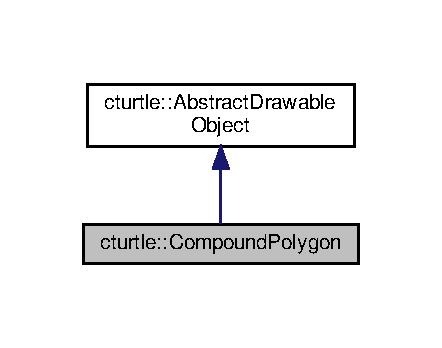
\includegraphics[width=212pt]{classcturtle_1_1CompoundPolygon__inherit__graph}
\end{center}
\end{figure}


Collaboration diagram for cturtle\+::Compound\+Polygon\+:\nopagebreak
\begin{figure}[H]
\begin{center}
\leavevmode
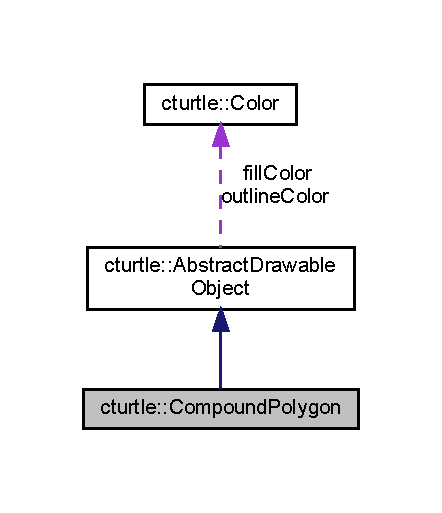
\includegraphics[width=212pt]{classcturtle_1_1CompoundPolygon__coll__graph}
\end{center}
\end{figure}
\doxysubsection*{Public Types}
\begin{DoxyCompactItemize}
\item 
\mbox{\Hypertarget{classcturtle_1_1CompoundPolygon_a10c24e9f65b586dec2c4173d2e4ddc2a}\label{classcturtle_1_1CompoundPolygon_a10c24e9f65b586dec2c4173d2e4ddc2a}} 
typedef std\+::pair$<$ \mbox{\hyperlink{classcturtle_1_1Transform}{Transform}}, std\+::unique\+\_\+ptr$<$ \mbox{\hyperlink{classcturtle_1_1AbstractDrawableObject}{Abstract\+Drawable\+Object}} $>$ $>$ {\bfseries component\+\_\+t}
\end{DoxyCompactItemize}
\doxysubsection*{Public Member Functions}
\begin{DoxyCompactItemize}
\item 
\mbox{\Hypertarget{classcturtle_1_1CompoundPolygon_a4ec03c8f5d2a8658893156ccadf0b347}\label{classcturtle_1_1CompoundPolygon_a4ec03c8f5d2a8658893156ccadf0b347}} 
{\bfseries Compound\+Polygon} (const \mbox{\hyperlink{classcturtle_1_1CompoundPolygon}{Compound\+Polygon}} \&\mbox{\hyperlink{classcturtle_1_1CompoundPolygon_af413f879d12105c9997b0e2e81e440a3}{copy}})
\item 
void \mbox{\hyperlink{classcturtle_1_1CompoundPolygon_a9b750af77967c4df01bab83785262e10}{addcomponent}} (const \mbox{\hyperlink{classcturtle_1_1AbstractDrawableObject}{Abstract\+Drawable\+Object}} \&obj, const \mbox{\hyperlink{classcturtle_1_1Transform}{Transform}} \&transform=\mbox{\hyperlink{classcturtle_1_1Transform}{Transform}}())
\begin{DoxyCompactList}\small\item\em Adds a component to this compound polygon. \end{DoxyCompactList}\item 
\mbox{\hyperlink{classcturtle_1_1AbstractDrawableObject}{Abstract\+Drawable\+Object}} $\ast$ \mbox{\hyperlink{classcturtle_1_1CompoundPolygon_af413f879d12105c9997b0e2e81e440a3}{copy}} () const
\item 
void \mbox{\hyperlink{classcturtle_1_1CompoundPolygon_aee485a61907d0a9c135344eadd5c52ad}{draw}} (const \mbox{\hyperlink{classcturtle_1_1Transform}{Transform}} \&t, Image \&img\+Ref) const
\end{DoxyCompactItemize}
\doxysubsection*{Protected Attributes}
\begin{DoxyCompactItemize}
\item 
\mbox{\Hypertarget{classcturtle_1_1CompoundPolygon_aac8199703a019ce5f09fd4ba96c95a39}\label{classcturtle_1_1CompoundPolygon_aac8199703a019ce5f09fd4ba96c95a39}} 
std\+::list$<$ component\+\_\+t $>$ {\bfseries components}
\end{DoxyCompactItemize}
\doxysubsection*{Additional Inherited Members}


\doxysubsection{Detailed Description}
a Compound \mbox{\hyperlink{classcturtle_1_1Polygon}{Polygon}} instance is composed from a number of smaller parts, which are each derived from \mbox{\hyperlink{classcturtle_1_1AbstractDrawableObject}{Abstract\+Drawable\+Object}}. Compound Polygons can have a variety of attachments. After the parts are assembled, the polygon is essentially read-\/only. These can be used to assemble several pieces of geometry into one object. These objects are self-\/contained and have ownership of all \mbox{\hyperlink{classcturtle_1_1AbstractDrawableObject}{Abstract\+Drawable\+Object}} instances they contain. 

\doxysubsection{Member Function Documentation}
\mbox{\Hypertarget{classcturtle_1_1CompoundPolygon_a9b750af77967c4df01bab83785262e10}\label{classcturtle_1_1CompoundPolygon_a9b750af77967c4df01bab83785262e10}} 
\index{cturtle::CompoundPolygon@{cturtle::CompoundPolygon}!addcomponent@{addcomponent}}
\index{addcomponent@{addcomponent}!cturtle::CompoundPolygon@{cturtle::CompoundPolygon}}
\doxysubsubsection{\texorpdfstring{addcomponent()}{addcomponent()}}
{\footnotesize\ttfamily void cturtle\+::\+Compound\+Polygon\+::addcomponent (\begin{DoxyParamCaption}\item[{const \mbox{\hyperlink{classcturtle_1_1AbstractDrawableObject}{Abstract\+Drawable\+Object}} \&}]{obj,  }\item[{const \mbox{\hyperlink{classcturtle_1_1Transform}{Transform}} \&}]{transform = {\ttfamily \mbox{\hyperlink{classcturtle_1_1Transform}{Transform}}()} }\end{DoxyParamCaption})\hspace{0.3cm}{\ttfamily [inline]}}



Adds a component to this compound polygon. 


\begin{DoxyParams}{Parameters}
{\em obj} & Object to copy and add. \\
\hline
{\em transform} & relative to root transform. \\
\hline
\end{DoxyParams}
\mbox{\Hypertarget{classcturtle_1_1CompoundPolygon_af413f879d12105c9997b0e2e81e440a3}\label{classcturtle_1_1CompoundPolygon_af413f879d12105c9997b0e2e81e440a3}} 
\index{cturtle::CompoundPolygon@{cturtle::CompoundPolygon}!copy@{copy}}
\index{copy@{copy}!cturtle::CompoundPolygon@{cturtle::CompoundPolygon}}
\doxysubsubsection{\texorpdfstring{copy()}{copy()}}
{\footnotesize\ttfamily \mbox{\hyperlink{classcturtle_1_1AbstractDrawableObject}{Abstract\+Drawable\+Object}}$\ast$ cturtle\+::\+Compound\+Polygon\+::copy (\begin{DoxyParamCaption}{ }\end{DoxyParamCaption}) const\hspace{0.3cm}{\ttfamily [inline]}, {\ttfamily [virtual]}}

Creates a copy of this Compound \mbox{\hyperlink{classcturtle_1_1Polygon}{Polygon}} allocated with the new keyword. This must be deleted at the responsibility of the invoker. 

Implements \mbox{\hyperlink{classcturtle_1_1AbstractDrawableObject_acff3437e999d281773b66e6cf2115372}{cturtle\+::\+Abstract\+Drawable\+Object}}.

\mbox{\Hypertarget{classcturtle_1_1CompoundPolygon_aee485a61907d0a9c135344eadd5c52ad}\label{classcturtle_1_1CompoundPolygon_aee485a61907d0a9c135344eadd5c52ad}} 
\index{cturtle::CompoundPolygon@{cturtle::CompoundPolygon}!draw@{draw}}
\index{draw@{draw}!cturtle::CompoundPolygon@{cturtle::CompoundPolygon}}
\doxysubsubsection{\texorpdfstring{draw()}{draw()}}
{\footnotesize\ttfamily void cturtle\+::\+Compound\+Polygon\+::draw (\begin{DoxyParamCaption}\item[{const \mbox{\hyperlink{classcturtle_1_1Transform}{Transform}} \&}]{t,  }\item[{Image \&}]{img\+Ref }\end{DoxyParamCaption}) const\hspace{0.3cm}{\ttfamily [inline]}, {\ttfamily [virtual]}}

Draws this \mbox{\hyperlink{classcturtle_1_1CompoundPolygon}{Compound\+Polygon}}. Disregards the \mbox{\hyperlink{classcturtle_1_1Color}{Color}} attribute in favor of the components\textquotesingle{} colors 

Implements \mbox{\hyperlink{classcturtle_1_1AbstractDrawableObject_a7b1ad1e9743d343e0fe577de3978bdad}{cturtle\+::\+Abstract\+Drawable\+Object}}.



The documentation for this class was generated from the following file\+:\begin{DoxyCompactItemize}
\item 
C\+Turtle.\+hpp\end{DoxyCompactItemize}

\hypertarget{structcturtle_1_1InputEvent}{}\doxysection{cturtle\+::Input\+Event Struct Reference}
\label{structcturtle_1_1InputEvent}\index{cturtle::InputEvent@{cturtle::InputEvent}}


The internally-\/used representation of an Input Event. Contains information pertaining to keyboard and mouse events, as well as callback pointers for either case.  




{\ttfamily \#include $<$CTurtle.\+hpp$>$}

\doxysubsection*{Public Attributes}
\begin{DoxyCompactItemize}
\item 
\mbox{\Hypertarget{structcturtle_1_1InputEvent_a0e599680d6faa3a406bd3322b299c5e5}\label{structcturtle_1_1InputEvent_a0e599680d6faa3a406bd3322b299c5e5}} 
bool {\bfseries type} = false
\item 
\mbox{\Hypertarget{structcturtle_1_1InputEvent_ad8ba7f1120fa5337edca37fd96d2d0ab}\label{structcturtle_1_1InputEvent_ad8ba7f1120fa5337edca37fd96d2d0ab}} 
int {\bfseries mX} = 0
\item 
\mbox{\Hypertarget{structcturtle_1_1InputEvent_a2862371531d61ed35e86930a46e5df62}\label{structcturtle_1_1InputEvent_a2862371531d61ed35e86930a46e5df62}} 
int {\bfseries mY} = 0
\item 
\mbox{\Hypertarget{structcturtle_1_1InputEvent_a3735358812d743ac70943b677a575c2e}\label{structcturtle_1_1InputEvent_a3735358812d743ac70943b677a575c2e}} 
void $\ast$ {\bfseries cb\+Pointer} = nullptr
\end{DoxyCompactItemize}


\doxysubsection{Detailed Description}
The internally-\/used representation of an Input Event. Contains information pertaining to keyboard and mouse events, as well as callback pointers for either case. 

The documentation for this struct was generated from the following file\+:\begin{DoxyCompactItemize}
\item 
CTurtle.\+hpp\end{DoxyCompactItemize}

\hypertarget{classcturtle_1_1InteractiveTurtleScreen}{}\section{cturtle\+:\+:Interactive\+Turtle\+Screen Class Reference}
\label{classcturtle_1_1InteractiveTurtleScreen}\index{cturtle\+::\+Interactive\+Turtle\+Screen@{cturtle\+::\+Interactive\+Turtle\+Screen}}


{\ttfamily \#include $<$C\+Turtle.\+hpp$>$}



Inheritance diagram for cturtle\+:\+:Interactive\+Turtle\+Screen\+:\nopagebreak
\begin{figure}[H]
\begin{center}
\leavevmode
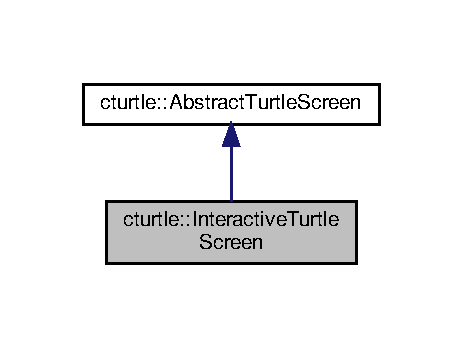
\includegraphics[width=222pt]{classcturtle_1_1InteractiveTurtleScreen__inherit__graph}
\end{center}
\end{figure}


Collaboration diagram for cturtle\+:\+:Interactive\+Turtle\+Screen\+:\nopagebreak
\begin{figure}[H]
\begin{center}
\leavevmode
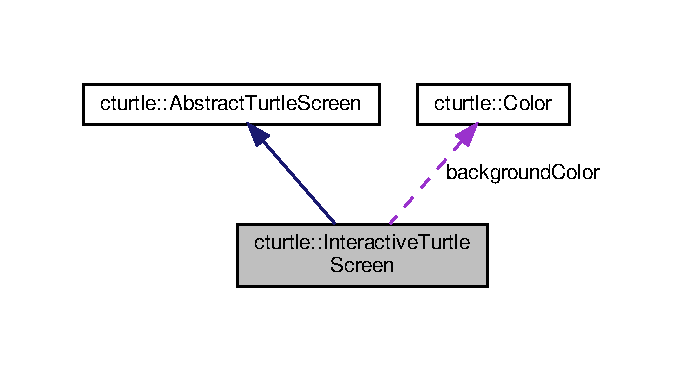
\includegraphics[width=328pt]{classcturtle_1_1InteractiveTurtleScreen__coll__graph}
\end{center}
\end{figure}
\subsection*{Public Member Functions}
\begin{DoxyCompactItemize}
\item 
\hyperlink{classcturtle_1_1InteractiveTurtleScreen_a3a2fc53b07958002992b8189a5af62f6}{Interactive\+Turtle\+Screen} ()
\item 
\hyperlink{classcturtle_1_1InteractiveTurtleScreen_ad65865be39cbe33c8614bb14f918058f}{Interactive\+Turtle\+Screen} (const std\+::string \&title)
\item 
\hyperlink{classcturtle_1_1InteractiveTurtleScreen_af9fb0672e3b17b2c07497de0b9ef99ee}{Interactive\+Turtle\+Screen} (int width, int height, const std\+::string \&title=\char`\"{}C\+Turtle\char`\"{})
\item 
\hyperlink{classcturtle_1_1InteractiveTurtleScreen_a74aecb49c64fd0035750c521d6029ccf}{$\sim$\+Interactive\+Turtle\+Screen} ()
\item 
void \hyperlink{classcturtle_1_1InteractiveTurtleScreen_ac6cbbcf714c490abb300cd6a931950f3}{tracer} (int countmax, unsigned int \hyperlink{classcturtle_1_1InteractiveTurtleScreen_a26338beec078bb1c29792cd658c1be71}{delay\+MS}=10)
\item 
void \hyperlink{classcturtle_1_1InteractiveTurtleScreen_acb5441704b45a01830d69df46a23732f}{bgcolor} (const \hyperlink{classcturtle_1_1Color}{Color} \&color)
\item 
\hyperlink{classcturtle_1_1Color}{Color} \hyperlink{classcturtle_1_1InteractiveTurtleScreen_a55289593218ba99904f7957700ef7dae}{bgcolor} () const
\item 
void \hyperlink{classcturtle_1_1InteractiveTurtleScreen_af681fbd6140ea760204fa9a1766725e3}{bgpic} (const Image \&img)
\begin{DoxyCompactList}\small\item\em Sets the background image of the display. Sets the background image. Please note that the background image takes precedence over background color. \end{DoxyCompactList}\item 
const Image \& \hyperlink{classcturtle_1_1InteractiveTurtleScreen_a57a90b8e6163e46c6fcb6f37b0b00e78}{bgpic} ()
\item 
bool \hyperlink{classcturtle_1_1InteractiveTurtleScreen_ad28f7c6e4058541a2c4258b4455fad74}{supports\+\_\+live\+\_\+animation} () const
\item 
void \hyperlink{classcturtle_1_1InteractiveTurtleScreen_a1c666afe65211cf9eedaffa17206a697}{mode} (Screen\+Mode mode)
\item 
Screen\+Mode \hyperlink{classcturtle_1_1InteractiveTurtleScreen_af65c66dbfe93fa748944f7a6d299080e}{mode} () const
\item 
\mbox{\Hypertarget{classcturtle_1_1InteractiveTurtleScreen_ae4e184867d7ed83c58e0ef9e730f4d73}\label{classcturtle_1_1InteractiveTurtleScreen_ae4e184867d7ed83c58e0ef9e730f4d73}} 
void \hyperlink{classcturtle_1_1InteractiveTurtleScreen_ae4e184867d7ed83c58e0ef9e730f4d73}{clearscreen} ()
\begin{DoxyCompactList}\small\item\em Clears this screen. Deletes all drawings and turtles, Resets the background to plain white, Clears all event bindings,. \end{DoxyCompactList}\item 
void \hyperlink{classcturtle_1_1InteractiveTurtleScreen_a60eecd547f88d1e52b1d0917693bffb8}{clear} ()
\item 
void \hyperlink{classcturtle_1_1InteractiveTurtleScreen_a06471bf6c8c02768fb0acd89649c72c2}{resetscreen} ()
\item 
void \hyperlink{classcturtle_1_1InteractiveTurtleScreen_a2863ede773ae592ad119b317b3704ce8}{reset} ()
\item 
\hyperlink{structcturtle_1_1ivec2}{ivec2} \hyperlink{classcturtle_1_1InteractiveTurtleScreen_a005b25693386718a6d80feeac677d255}{screensize} (\hyperlink{classcturtle_1_1Color}{Color} \&bg)
\item 
\hyperlink{structcturtle_1_1ivec2}{ivec2} \hyperlink{classcturtle_1_1InteractiveTurtleScreen_a1263d763eb9ef1b39f2e8c0a445d6a85}{screensize} ()
\item 
void \hyperlink{classcturtle_1_1InteractiveTurtleScreen_adfefb43645347feb832072f8fc8da144}{update} (bool invalidate\+Draw=false, bool process\+Input=true)
\item 
void \hyperlink{classcturtle_1_1InteractiveTurtleScreen_a6e32b852cbd029d6649107d838c798a9}{delay} (unsigned int ms)
\item 
unsigned int \hyperlink{classcturtle_1_1InteractiveTurtleScreen_a2776d2a194e14b7adbc94ce502ee9409}{delay} ()
\item 
int \hyperlink{classcturtle_1_1InteractiveTurtleScreen_aefeb4e90fae07d043677f3dee9a29026}{window\+\_\+width} () const
\item 
int \hyperlink{classcturtle_1_1InteractiveTurtleScreen_a259883332b284e3b8a97b5bfb74f988d}{window\+\_\+height} () const
\item 
void \hyperlink{classcturtle_1_1InteractiveTurtleScreen_ab0ded9c577f523ca45240e036318553e}{save} (const std\+::string \&file)
\item 
void \hyperlink{classcturtle_1_1InteractiveTurtleScreen_a0b6a0f18333312f7d502b3d9a511143e}{mainloop} ()
\item 
void \hyperlink{classcturtle_1_1InteractiveTurtleScreen_a045b2cc0c8869140015abcc11226a714}{bye} ()
\item 
Image \& \hyperlink{classcturtle_1_1InteractiveTurtleScreen_ad2156553b1af3d0ab4527d8ddbda5d61}{getcanvas} ()
\item 
cimg\+::\+C\+Img\+Display \& \hyperlink{classcturtle_1_1InteractiveTurtleScreen_a0ea57bab0cb93f0fa4629747bddbab30}{internaldisplay} ()
\item 
bool \hyperlink{classcturtle_1_1InteractiveTurtleScreen_ab1809a5a10cb3afaa330d6ba2ee5bb49}{isclosed} ()
\item 
void \hyperlink{classcturtle_1_1InteractiveTurtleScreen_ad0e307da3f48e9e1ce6660c975ca3854}{redraw} (bool invalidate=false)
\item 
\hyperlink{classcturtle_1_1Transform}{Transform} \hyperlink{classcturtle_1_1InteractiveTurtleScreen_a6c81f204488e1ebe8180504990e559dc}{screentransform} () const
\item 
void \hyperlink{classcturtle_1_1InteractiveTurtleScreen_a997c82f379c6c90e2f1d2336db8bc1fc}{onkeypress} (Key\+Func func, Keyboard\+Key key)
\begin{DoxyCompactList}\small\item\em Adds an additional \char`\"{}on press\char`\"{} key binding for the specified key. \end{DoxyCompactList}\item 
virtual void \hyperlink{classcturtle_1_1InteractiveTurtleScreen_a313943b2ae07b9a67ae0681fbadc2085}{onkeyrelease} (Key\+Func func, Keyboard\+Key key)
\begin{DoxyCompactList}\small\item\em Adds an additional \char`\"{}on press\char`\"{} key binding for the specified key. \end{DoxyCompactList}\item 
void \hyperlink{classcturtle_1_1InteractiveTurtleScreen_a4273782c35444bc35afb0a8ea0f6a168}{presskey} (Keyboard\+Key key)
\begin{DoxyCompactList}\small\item\em Simulates a key \char`\"{}on press\char`\"{} event. \end{DoxyCompactList}\item 
void \hyperlink{classcturtle_1_1InteractiveTurtleScreen_a31a3f4a793acd97e8e6e8a42a7c7c885}{releasekey} (Keyboard\+Key key)
\begin{DoxyCompactList}\small\item\em Simulates a key \char`\"{}on release\char`\"{} event. \end{DoxyCompactList}\item 
void \hyperlink{classcturtle_1_1InteractiveTurtleScreen_a05410a8f835e296f8ffca90ca3b0da24}{onclick} (Mouse\+Func func, Mouse\+Button button=M\+O\+U\+S\+E\+B\+\_\+\+L\+E\+FT)
\begin{DoxyCompactList}\small\item\em Adds an additional \char`\"{}on click\char`\"{} mouse binding for the specified button. \end{DoxyCompactList}\item 
void \hyperlink{classcturtle_1_1InteractiveTurtleScreen_a8fcbf045a17072cc8dda12f20035bb97}{click} (int x, int y, Mouse\+Button button)
\item 
void \hyperlink{classcturtle_1_1InteractiveTurtleScreen_a793b9bc88ac4ce7c5b6d8b6fbc96a3fe}{click} (const \hyperlink{structcturtle_1_1ivec2}{Point} \&pt, Mouse\+Button button)
\item 
void \hyperlink{classcturtle_1_1InteractiveTurtleScreen_ab60ddd682f7fa7df3635f936bcfd2f70}{ontimer} (Timer\+Func func, unsigned int time)
\begin{DoxyCompactList}\small\item\em Adds a timer function to be called every N milliseconds. \end{DoxyCompactList}\item 
void \hyperlink{classcturtle_1_1InteractiveTurtleScreen_ada27fc4b13ce99e45531ccf703d1fb8a}{exitonclick} ()
\item 
void \hyperlink{classcturtle_1_1InteractiveTurtleScreen_ab9696275e4a7b10225cfe10e48fd8c89}{add} (\hyperlink{classcturtle_1_1Turtle}{Turtle} \&turtle)
\item 
std\+::list$<$ \hyperlink{structcturtle_1_1SceneObject}{Scene\+Object} $>$ \& \hyperlink{classcturtle_1_1InteractiveTurtleScreen_aa1bd826458a718e7605424d5767f79c9}{get\+Scene} ()
\item 
\hyperlink{classcturtle_1_1AbstractDrawableObject}{Abstract\+Drawable\+Object} \& \hyperlink{classcturtle_1_1InteractiveTurtleScreen_ae855fb3d2acd831ce751e9387b8edc06}{shape} (const std\+::string \&name)
\end{DoxyCompactItemize}
\subsection*{Protected Member Functions}
\begin{DoxyCompactItemize}
\item 
void \hyperlink{classcturtle_1_1InteractiveTurtleScreen_aa7c436f89d052e42500356ee5f479776}{init\+Event\+Thread} ()
\end{DoxyCompactItemize}
\subsection*{Protected Attributes}
\begin{DoxyCompactItemize}
\item 
cimg\+::\+C\+Img\+Display \hyperlink{classcturtle_1_1InteractiveTurtleScreen_a5ab4e006c97cfd1610dc565188e9c9b0}{display}
\item 
Image \hyperlink{classcturtle_1_1InteractiveTurtleScreen_a5231bfae24c5e5387059fccffa9a7170}{canvas}
\item 
\mbox{\Hypertarget{classcturtle_1_1InteractiveTurtleScreen_a3a6e3d9249b40dccc5a4e4f0f1dd4075}\label{classcturtle_1_1InteractiveTurtleScreen_a3a6e3d9249b40dccc5a4e4f0f1dd4075}} 
Image {\bfseries turtle\+Composite}
\item 
int \hyperlink{classcturtle_1_1InteractiveTurtleScreen_afd74d43945f4eb82bb71e0d2b4a72a50}{last\+Total\+Objects} = 0
\item 
\hyperlink{classcturtle_1_1Color}{Color} \hyperlink{classcturtle_1_1InteractiveTurtleScreen_a3cc73fa2f1e0f2579a5bc1917396e023}{background\+Color} = \hyperlink{classcturtle_1_1Color}{Color}(\char`\"{}white\char`\"{})
\item 
Image \hyperlink{classcturtle_1_1InteractiveTurtleScreen_a139236df336d32f5cb44ab8ccfb16475}{background\+Image}
\item 
Screen\+Mode \hyperlink{classcturtle_1_1InteractiveTurtleScreen_a6fd7fc060f0e4adcc08ab1e43e758c49}{cur\+Mode} = S\+M\+\_\+\+S\+T\+A\+N\+D\+A\+RD
\item 
long int \hyperlink{classcturtle_1_1InteractiveTurtleScreen_a26338beec078bb1c29792cd658c1be71}{delay\+MS} = 10
\item 
int \hyperlink{classcturtle_1_1InteractiveTurtleScreen_a39c21ce1ed1de241676ae329ecd962b8}{redraw\+Counter} = 0
\item 
int \hyperlink{classcturtle_1_1InteractiveTurtleScreen_a7cf0a4e382da4be238be3f9d3510b4e7}{redraw\+Counter\+Max} = 1
\item 
std\+::list$<$ \hyperlink{structcturtle_1_1SceneObject}{Scene\+Object} $>$ \hyperlink{classcturtle_1_1InteractiveTurtleScreen_abaea1170c38b5e79865841834c50718d}{objects}
\item 
std\+::list$<$ \hyperlink{classcturtle_1_1Turtle}{Turtle} $\ast$ $>$ \hyperlink{classcturtle_1_1InteractiveTurtleScreen_ae227fdb4ee9017964e314d6e0c76cee4}{turtles}
\item 
std\+::unique\+\_\+ptr$<$ std\+::thread $>$ \hyperlink{classcturtle_1_1InteractiveTurtleScreen_ace652d27f7e65ee15cd4dab7074874d2}{event\+Thread}
\item 
std\+::list$<$ \hyperlink{structcturtle_1_1InputEvent}{Input\+Event} $>$ \hyperlink{classcturtle_1_1InteractiveTurtleScreen_a1573f71b0a5125a4cdfd5cbf8096f271}{cached\+Events}
\item 
bool \hyperlink{classcturtle_1_1InteractiveTurtleScreen_a800665243e7f329177b4bfa12213a063}{kill\+Event\+Thread} = false
\item 
std\+::mutex \hyperlink{classcturtle_1_1InteractiveTurtleScreen_ab31b4060c56cf038540277f041a4bf4a}{event\+Cache\+Mutex}
\item 
std\+::unordered\+\_\+map$<$ Keyboard\+Key, std\+::list$<$ Key\+Func $>$ $>$ {\bfseries key\+Bindings} \mbox{[}2\mbox{]}
\item 
std\+::list$<$ Mouse\+Func $>$ {\bfseries mouse\+Bindings} \mbox{[}3\mbox{]}
\item 
\mbox{\Hypertarget{classcturtle_1_1InteractiveTurtleScreen_a4df96b64c8abe7fa20aba4b376744136}\label{classcturtle_1_1InteractiveTurtleScreen_a4df96b64c8abe7fa20aba4b376744136}} 
std\+::list$<$ std\+::tuple$<$ Timer\+Func, uint64\+\_\+t, uint64\+\_\+t $>$ $>$ {\bfseries timer\+Bindings}
\item 
std\+::unordered\+\_\+map$<$ std\+::string, \hyperlink{classcturtle_1_1Polygon}{Polygon} $>$ {\bfseries shapes}
\end{DoxyCompactItemize}


\subsection{Detailed Description}
\hyperlink{classcturtle_1_1InteractiveTurtleScreen}{Interactive\+Turtle\+Screen} Holds and maintains facilities in relation to displaying turtles and consuming input events from users through callbacks. This includes holding the actual data for a given scene after being populated by \hyperlink{classcturtle_1_1Turtle}{Turtle}. It layers draw calls in the order they are called, independent of whatever \hyperlink{classcturtle_1_1Turtle}{Turtle} object creates it.

\begin{DoxySeeAlso}{See also}
\hyperlink{classcturtle_1_1Turtle}{Turtle} 
\end{DoxySeeAlso}


\subsection{Constructor \& Destructor Documentation}
\mbox{\Hypertarget{classcturtle_1_1InteractiveTurtleScreen_a3a2fc53b07958002992b8189a5af62f6}\label{classcturtle_1_1InteractiveTurtleScreen_a3a2fc53b07958002992b8189a5af62f6}} 
\index{cturtle\+::\+Interactive\+Turtle\+Screen@{cturtle\+::\+Interactive\+Turtle\+Screen}!Interactive\+Turtle\+Screen@{Interactive\+Turtle\+Screen}}
\index{Interactive\+Turtle\+Screen@{Interactive\+Turtle\+Screen}!cturtle\+::\+Interactive\+Turtle\+Screen@{cturtle\+::\+Interactive\+Turtle\+Screen}}
\subsubsection{\texorpdfstring{Interactive\+Turtle\+Screen()}{InteractiveTurtleScreen()}\hspace{0.1cm}{\footnotesize\ttfamily [1/3]}}
{\footnotesize\ttfamily cturtle\+::\+Interactive\+Turtle\+Screen\+::\+Interactive\+Turtle\+Screen (\begin{DoxyParamCaption}{ }\end{DoxyParamCaption})\hspace{0.3cm}{\ttfamily [inline]}}

Empty constructor. Assigns an 800 x 600 pixel display with a title of \char`\"{}\+C\+Turtle\char`\"{}. \mbox{\Hypertarget{classcturtle_1_1InteractiveTurtleScreen_ad65865be39cbe33c8614bb14f918058f}\label{classcturtle_1_1InteractiveTurtleScreen_ad65865be39cbe33c8614bb14f918058f}} 
\index{cturtle\+::\+Interactive\+Turtle\+Screen@{cturtle\+::\+Interactive\+Turtle\+Screen}!Interactive\+Turtle\+Screen@{Interactive\+Turtle\+Screen}}
\index{Interactive\+Turtle\+Screen@{Interactive\+Turtle\+Screen}!cturtle\+::\+Interactive\+Turtle\+Screen@{cturtle\+::\+Interactive\+Turtle\+Screen}}
\subsubsection{\texorpdfstring{Interactive\+Turtle\+Screen()}{InteractiveTurtleScreen()}\hspace{0.1cm}{\footnotesize\ttfamily [2/3]}}
{\footnotesize\ttfamily cturtle\+::\+Interactive\+Turtle\+Screen\+::\+Interactive\+Turtle\+Screen (\begin{DoxyParamCaption}\item[{const std\+::string \&}]{title }\end{DoxyParamCaption})\hspace{0.3cm}{\ttfamily [inline]}}

Title constructor. Assigns an 800 x 600 pixel display with a specified title. 
\begin{DoxyParams}{Parameters}
{\em title} & The title to assign the display with. \\
\hline
\end{DoxyParams}
\mbox{\Hypertarget{classcturtle_1_1InteractiveTurtleScreen_af9fb0672e3b17b2c07497de0b9ef99ee}\label{classcturtle_1_1InteractiveTurtleScreen_af9fb0672e3b17b2c07497de0b9ef99ee}} 
\index{cturtle\+::\+Interactive\+Turtle\+Screen@{cturtle\+::\+Interactive\+Turtle\+Screen}!Interactive\+Turtle\+Screen@{Interactive\+Turtle\+Screen}}
\index{Interactive\+Turtle\+Screen@{Interactive\+Turtle\+Screen}!cturtle\+::\+Interactive\+Turtle\+Screen@{cturtle\+::\+Interactive\+Turtle\+Screen}}
\subsubsection{\texorpdfstring{Interactive\+Turtle\+Screen()}{InteractiveTurtleScreen()}\hspace{0.1cm}{\footnotesize\ttfamily [3/3]}}
{\footnotesize\ttfamily cturtle\+::\+Interactive\+Turtle\+Screen\+::\+Interactive\+Turtle\+Screen (\begin{DoxyParamCaption}\item[{int}]{width,  }\item[{int}]{height,  }\item[{const std\+::string \&}]{title = {\ttfamily \char`\"{}CTurtle\char`\"{}} }\end{DoxyParamCaption})\hspace{0.3cm}{\ttfamily [inline]}}

Width, height, and title constructor. Assigns the display with the specified dimensions, in pixels, and assigns the display the specified title. 
\begin{DoxyParams}{Parameters}
{\em width} & The width of the display, in pixels. \\
\hline
{\em height} & The height of the display, in pixels. \\
\hline
{\em title} & The title of the display. \\
\hline
\end{DoxyParams}
\mbox{\Hypertarget{classcturtle_1_1InteractiveTurtleScreen_a74aecb49c64fd0035750c521d6029ccf}\label{classcturtle_1_1InteractiveTurtleScreen_a74aecb49c64fd0035750c521d6029ccf}} 
\index{cturtle\+::\+Interactive\+Turtle\+Screen@{cturtle\+::\+Interactive\+Turtle\+Screen}!````~Interactive\+Turtle\+Screen@{$\sim$\+Interactive\+Turtle\+Screen}}
\index{````~Interactive\+Turtle\+Screen@{$\sim$\+Interactive\+Turtle\+Screen}!cturtle\+::\+Interactive\+Turtle\+Screen@{cturtle\+::\+Interactive\+Turtle\+Screen}}
\subsubsection{\texorpdfstring{$\sim$\+Interactive\+Turtle\+Screen()}{~InteractiveTurtleScreen()}}
{\footnotesize\ttfamily cturtle\+::\+Interactive\+Turtle\+Screen\+::$\sim$\+Interactive\+Turtle\+Screen (\begin{DoxyParamCaption}{ }\end{DoxyParamCaption})\hspace{0.3cm}{\ttfamily [inline]}}

Destructor. Calls \char`\"{}bye\char`\"{} function. 

\subsection{Member Function Documentation}
\mbox{\Hypertarget{classcturtle_1_1InteractiveTurtleScreen_ab9696275e4a7b10225cfe10e48fd8c89}\label{classcturtle_1_1InteractiveTurtleScreen_ab9696275e4a7b10225cfe10e48fd8c89}} 
\index{cturtle\+::\+Interactive\+Turtle\+Screen@{cturtle\+::\+Interactive\+Turtle\+Screen}!add@{add}}
\index{add@{add}!cturtle\+::\+Interactive\+Turtle\+Screen@{cturtle\+::\+Interactive\+Turtle\+Screen}}
\subsubsection{\texorpdfstring{add()}{add()}}
{\footnotesize\ttfamily void cturtle\+::\+Interactive\+Turtle\+Screen\+::add (\begin{DoxyParamCaption}\item[{\hyperlink{classcturtle_1_1Turtle}{Turtle} \&}]{turtle }\end{DoxyParamCaption})\hspace{0.3cm}{\ttfamily [inline]}, {\ttfamily [virtual]}}

Adds the specified turtle to this screen. 

Implements \hyperlink{classcturtle_1_1AbstractTurtleScreen}{cturtle\+::\+Abstract\+Turtle\+Screen}.

\mbox{\Hypertarget{classcturtle_1_1InteractiveTurtleScreen_acb5441704b45a01830d69df46a23732f}\label{classcturtle_1_1InteractiveTurtleScreen_acb5441704b45a01830d69df46a23732f}} 
\index{cturtle\+::\+Interactive\+Turtle\+Screen@{cturtle\+::\+Interactive\+Turtle\+Screen}!bgcolor@{bgcolor}}
\index{bgcolor@{bgcolor}!cturtle\+::\+Interactive\+Turtle\+Screen@{cturtle\+::\+Interactive\+Turtle\+Screen}}
\subsubsection{\texorpdfstring{bgcolor()}{bgcolor()}\hspace{0.1cm}{\footnotesize\ttfamily [1/2]}}
{\footnotesize\ttfamily void cturtle\+::\+Interactive\+Turtle\+Screen\+::bgcolor (\begin{DoxyParamCaption}\item[{const \hyperlink{classcturtle_1_1Color}{Color} \&}]{color }\end{DoxyParamCaption})\hspace{0.3cm}{\ttfamily [inline]}, {\ttfamily [virtual]}}

Sets the background color of the screen. Please note that, if there is a background image, this color is not applied until it is removed. 
\begin{DoxyParams}{Parameters}
{\em color} & The background color. \\
\hline
\end{DoxyParams}
\begin{DoxySeeAlso}{See also}
bgpic(image) 
\end{DoxySeeAlso}


Implements \hyperlink{classcturtle_1_1AbstractTurtleScreen}{cturtle\+::\+Abstract\+Turtle\+Screen}.

\mbox{\Hypertarget{classcturtle_1_1InteractiveTurtleScreen_a55289593218ba99904f7957700ef7dae}\label{classcturtle_1_1InteractiveTurtleScreen_a55289593218ba99904f7957700ef7dae}} 
\index{cturtle\+::\+Interactive\+Turtle\+Screen@{cturtle\+::\+Interactive\+Turtle\+Screen}!bgcolor@{bgcolor}}
\index{bgcolor@{bgcolor}!cturtle\+::\+Interactive\+Turtle\+Screen@{cturtle\+::\+Interactive\+Turtle\+Screen}}
\subsubsection{\texorpdfstring{bgcolor()}{bgcolor()}\hspace{0.1cm}{\footnotesize\ttfamily [2/2]}}
{\footnotesize\ttfamily \hyperlink{classcturtle_1_1Color}{Color} cturtle\+::\+Interactive\+Turtle\+Screen\+::bgcolor (\begin{DoxyParamCaption}{ }\end{DoxyParamCaption}) const\hspace{0.3cm}{\ttfamily [inline]}, {\ttfamily [virtual]}}

Returns the background color of the screen. \begin{DoxyReturn}{Returns}
The background color of the screen. 
\end{DoxyReturn}


Implements \hyperlink{classcturtle_1_1AbstractTurtleScreen}{cturtle\+::\+Abstract\+Turtle\+Screen}.

\mbox{\Hypertarget{classcturtle_1_1InteractiveTurtleScreen_af681fbd6140ea760204fa9a1766725e3}\label{classcturtle_1_1InteractiveTurtleScreen_af681fbd6140ea760204fa9a1766725e3}} 
\index{cturtle\+::\+Interactive\+Turtle\+Screen@{cturtle\+::\+Interactive\+Turtle\+Screen}!bgpic@{bgpic}}
\index{bgpic@{bgpic}!cturtle\+::\+Interactive\+Turtle\+Screen@{cturtle\+::\+Interactive\+Turtle\+Screen}}
\subsubsection{\texorpdfstring{bgpic()}{bgpic()}\hspace{0.1cm}{\footnotesize\ttfamily [1/2]}}
{\footnotesize\ttfamily void cturtle\+::\+Interactive\+Turtle\+Screen\+::bgpic (\begin{DoxyParamCaption}\item[{const Image \&}]{img }\end{DoxyParamCaption})\hspace{0.3cm}{\ttfamily [inline]}}



Sets the background image of the display. Sets the background image. Please note that the background image takes precedence over background color. 


\begin{DoxyParams}{Parameters}
{\em img} & The background image. \\
\hline
\end{DoxyParams}
\mbox{\Hypertarget{classcturtle_1_1InteractiveTurtleScreen_a57a90b8e6163e46c6fcb6f37b0b00e78}\label{classcturtle_1_1InteractiveTurtleScreen_a57a90b8e6163e46c6fcb6f37b0b00e78}} 
\index{cturtle\+::\+Interactive\+Turtle\+Screen@{cturtle\+::\+Interactive\+Turtle\+Screen}!bgpic@{bgpic}}
\index{bgpic@{bgpic}!cturtle\+::\+Interactive\+Turtle\+Screen@{cturtle\+::\+Interactive\+Turtle\+Screen}}
\subsubsection{\texorpdfstring{bgpic()}{bgpic()}\hspace{0.1cm}{\footnotesize\ttfamily [2/2]}}
{\footnotesize\ttfamily const Image\& cturtle\+::\+Interactive\+Turtle\+Screen\+::bgpic (\begin{DoxyParamCaption}{ }\end{DoxyParamCaption})\hspace{0.3cm}{\ttfamily [inline]}}

Returns a const reference to the background image. \mbox{\Hypertarget{classcturtle_1_1InteractiveTurtleScreen_a045b2cc0c8869140015abcc11226a714}\label{classcturtle_1_1InteractiveTurtleScreen_a045b2cc0c8869140015abcc11226a714}} 
\index{cturtle\+::\+Interactive\+Turtle\+Screen@{cturtle\+::\+Interactive\+Turtle\+Screen}!bye@{bye}}
\index{bye@{bye}!cturtle\+::\+Interactive\+Turtle\+Screen@{cturtle\+::\+Interactive\+Turtle\+Screen}}
\subsubsection{\texorpdfstring{bye()}{bye()}}
{\footnotesize\ttfamily void cturtle\+::\+Interactive\+Turtle\+Screen\+::bye (\begin{DoxyParamCaption}{ }\end{DoxyParamCaption})\hspace{0.3cm}{\ttfamily [inline]}, {\ttfamily [virtual]}}

Resets and closes this display. 

Implements \hyperlink{classcturtle_1_1AbstractTurtleScreen}{cturtle\+::\+Abstract\+Turtle\+Screen}.

\mbox{\Hypertarget{classcturtle_1_1InteractiveTurtleScreen_a60eecd547f88d1e52b1d0917693bffb8}\label{classcturtle_1_1InteractiveTurtleScreen_a60eecd547f88d1e52b1d0917693bffb8}} 
\index{cturtle\+::\+Interactive\+Turtle\+Screen@{cturtle\+::\+Interactive\+Turtle\+Screen}!clear@{clear}}
\index{clear@{clear}!cturtle\+::\+Interactive\+Turtle\+Screen@{cturtle\+::\+Interactive\+Turtle\+Screen}}
\subsubsection{\texorpdfstring{clear()}{clear()}}
{\footnotesize\ttfamily void cturtle\+::\+Interactive\+Turtle\+Screen\+::clear (\begin{DoxyParamCaption}{ }\end{DoxyParamCaption})\hspace{0.3cm}{\ttfamily [inline]}}

Alias for clearscreen function \begin{DoxySeeAlso}{See also}
\hyperlink{classcturtle_1_1InteractiveTurtleScreen_ae4e184867d7ed83c58e0ef9e730f4d73}{clearscreen()} 
\end{DoxySeeAlso}
\mbox{\Hypertarget{classcturtle_1_1InteractiveTurtleScreen_a8fcbf045a17072cc8dda12f20035bb97}\label{classcturtle_1_1InteractiveTurtleScreen_a8fcbf045a17072cc8dda12f20035bb97}} 
\index{cturtle\+::\+Interactive\+Turtle\+Screen@{cturtle\+::\+Interactive\+Turtle\+Screen}!click@{click}}
\index{click@{click}!cturtle\+::\+Interactive\+Turtle\+Screen@{cturtle\+::\+Interactive\+Turtle\+Screen}}
\subsubsection{\texorpdfstring{click()}{click()}\hspace{0.1cm}{\footnotesize\ttfamily [1/2]}}
{\footnotesize\ttfamily void cturtle\+::\+Interactive\+Turtle\+Screen\+::click (\begin{DoxyParamCaption}\item[{int}]{x,  }\item[{int}]{y,  }\item[{Mouse\+Button}]{button }\end{DoxyParamCaption})\hspace{0.3cm}{\ttfamily [inline]}}

Calls all previously added mouse button call-\/backs. 
\begin{DoxyParams}{Parameters}
{\em x} & The X coordinate at which to press. \\
\hline
{\em y} & The Y coordinate at which to press. \\
\hline
{\em button} & The button to simulate being pressed. \\
\hline
\end{DoxyParams}
\mbox{\Hypertarget{classcturtle_1_1InteractiveTurtleScreen_a793b9bc88ac4ce7c5b6d8b6fbc96a3fe}\label{classcturtle_1_1InteractiveTurtleScreen_a793b9bc88ac4ce7c5b6d8b6fbc96a3fe}} 
\index{cturtle\+::\+Interactive\+Turtle\+Screen@{cturtle\+::\+Interactive\+Turtle\+Screen}!click@{click}}
\index{click@{click}!cturtle\+::\+Interactive\+Turtle\+Screen@{cturtle\+::\+Interactive\+Turtle\+Screen}}
\subsubsection{\texorpdfstring{click()}{click()}\hspace{0.1cm}{\footnotesize\ttfamily [2/2]}}
{\footnotesize\ttfamily void cturtle\+::\+Interactive\+Turtle\+Screen\+::click (\begin{DoxyParamCaption}\item[{const \hyperlink{structcturtle_1_1ivec2}{Point} \&}]{pt,  }\item[{Mouse\+Button}]{button }\end{DoxyParamCaption})\hspace{0.3cm}{\ttfamily [inline]}}





Calls all previously added mouse button call-\/backs. 
\begin{DoxyParams}{Parameters}
{\em x} & The X coordinate at which to press. \\
\hline
{\em y} & The Y coordinate at which to press. \\
\hline
{\em button} & The button to simulate being pressed. \\
\hline
\end{DoxyParams}
\mbox{\Hypertarget{classcturtle_1_1InteractiveTurtleScreen_a6e32b852cbd029d6649107d838c798a9}\label{classcturtle_1_1InteractiveTurtleScreen_a6e32b852cbd029d6649107d838c798a9}} 
\index{cturtle\+::\+Interactive\+Turtle\+Screen@{cturtle\+::\+Interactive\+Turtle\+Screen}!delay@{delay}}
\index{delay@{delay}!cturtle\+::\+Interactive\+Turtle\+Screen@{cturtle\+::\+Interactive\+Turtle\+Screen}}
\subsubsection{\texorpdfstring{delay()}{delay()}\hspace{0.1cm}{\footnotesize\ttfamily [1/2]}}
{\footnotesize\ttfamily void cturtle\+::\+Interactive\+Turtle\+Screen\+::delay (\begin{DoxyParamCaption}\item[{unsigned int}]{ms }\end{DoxyParamCaption})\hspace{0.3cm}{\ttfamily [inline]}, {\ttfamily [virtual]}}

Sets the delay set between turtle commands. 

Implements \hyperlink{classcturtle_1_1AbstractTurtleScreen}{cturtle\+::\+Abstract\+Turtle\+Screen}.

\mbox{\Hypertarget{classcturtle_1_1InteractiveTurtleScreen_a2776d2a194e14b7adbc94ce502ee9409}\label{classcturtle_1_1InteractiveTurtleScreen_a2776d2a194e14b7adbc94ce502ee9409}} 
\index{cturtle\+::\+Interactive\+Turtle\+Screen@{cturtle\+::\+Interactive\+Turtle\+Screen}!delay@{delay}}
\index{delay@{delay}!cturtle\+::\+Interactive\+Turtle\+Screen@{cturtle\+::\+Interactive\+Turtle\+Screen}}
\subsubsection{\texorpdfstring{delay()}{delay()}\hspace{0.1cm}{\footnotesize\ttfamily [2/2]}}
{\footnotesize\ttfamily unsigned int cturtle\+::\+Interactive\+Turtle\+Screen\+::delay (\begin{DoxyParamCaption}{ }\end{DoxyParamCaption})\hspace{0.3cm}{\ttfamily [inline]}, {\ttfamily [virtual]}}

Returns the delay set between screen swaps in milliseconds. 

Implements \hyperlink{classcturtle_1_1AbstractTurtleScreen}{cturtle\+::\+Abstract\+Turtle\+Screen}.

\mbox{\Hypertarget{classcturtle_1_1InteractiveTurtleScreen_ada27fc4b13ce99e45531ccf703d1fb8a}\label{classcturtle_1_1InteractiveTurtleScreen_ada27fc4b13ce99e45531ccf703d1fb8a}} 
\index{cturtle\+::\+Interactive\+Turtle\+Screen@{cturtle\+::\+Interactive\+Turtle\+Screen}!exitonclick@{exitonclick}}
\index{exitonclick@{exitonclick}!cturtle\+::\+Interactive\+Turtle\+Screen@{cturtle\+::\+Interactive\+Turtle\+Screen}}
\subsubsection{\texorpdfstring{exitonclick()}{exitonclick()}}
{\footnotesize\ttfamily void cturtle\+::\+Interactive\+Turtle\+Screen\+::exitonclick (\begin{DoxyParamCaption}{ }\end{DoxyParamCaption})\hspace{0.3cm}{\ttfamily [inline]}}

Binds the \char`\"{}bye\char`\"{} function to the onclick event for the left mouse button. \mbox{\Hypertarget{classcturtle_1_1InteractiveTurtleScreen_ad2156553b1af3d0ab4527d8ddbda5d61}\label{classcturtle_1_1InteractiveTurtleScreen_ad2156553b1af3d0ab4527d8ddbda5d61}} 
\index{cturtle\+::\+Interactive\+Turtle\+Screen@{cturtle\+::\+Interactive\+Turtle\+Screen}!getcanvas@{getcanvas}}
\index{getcanvas@{getcanvas}!cturtle\+::\+Interactive\+Turtle\+Screen@{cturtle\+::\+Interactive\+Turtle\+Screen}}
\subsubsection{\texorpdfstring{getcanvas()}{getcanvas()}}
{\footnotesize\ttfamily Image\& cturtle\+::\+Interactive\+Turtle\+Screen\+::getcanvas (\begin{DoxyParamCaption}{ }\end{DoxyParamCaption})\hspace{0.3cm}{\ttfamily [inline]}, {\ttfamily [virtual]}}

Returns the canvas image used by this screen. 

Implements \hyperlink{classcturtle_1_1AbstractTurtleScreen}{cturtle\+::\+Abstract\+Turtle\+Screen}.

\mbox{\Hypertarget{classcturtle_1_1InteractiveTurtleScreen_aa1bd826458a718e7605424d5767f79c9}\label{classcturtle_1_1InteractiveTurtleScreen_aa1bd826458a718e7605424d5767f79c9}} 
\index{cturtle\+::\+Interactive\+Turtle\+Screen@{cturtle\+::\+Interactive\+Turtle\+Screen}!get\+Scene@{get\+Scene}}
\index{get\+Scene@{get\+Scene}!cturtle\+::\+Interactive\+Turtle\+Screen@{cturtle\+::\+Interactive\+Turtle\+Screen}}
\subsubsection{\texorpdfstring{get\+Scene()}{getScene()}}
{\footnotesize\ttfamily std\+::list$<$\hyperlink{structcturtle_1_1SceneObject}{Scene\+Object}$>$\& cturtle\+::\+Interactive\+Turtle\+Screen\+::get\+Scene (\begin{DoxyParamCaption}{ }\end{DoxyParamCaption})\hspace{0.3cm}{\ttfamily [inline]}, {\ttfamily [virtual]}}

Returns a reference to the list of scene objects. This list is used to redraw the screen. 

Implements \hyperlink{classcturtle_1_1AbstractTurtleScreen}{cturtle\+::\+Abstract\+Turtle\+Screen}.

\mbox{\Hypertarget{classcturtle_1_1InteractiveTurtleScreen_aa7c436f89d052e42500356ee5f479776}\label{classcturtle_1_1InteractiveTurtleScreen_aa7c436f89d052e42500356ee5f479776}} 
\index{cturtle\+::\+Interactive\+Turtle\+Screen@{cturtle\+::\+Interactive\+Turtle\+Screen}!init\+Event\+Thread@{init\+Event\+Thread}}
\index{init\+Event\+Thread@{init\+Event\+Thread}!cturtle\+::\+Interactive\+Turtle\+Screen@{cturtle\+::\+Interactive\+Turtle\+Screen}}
\subsubsection{\texorpdfstring{init\+Event\+Thread()}{initEventThread()}}
{\footnotesize\ttfamily void cturtle\+::\+Interactive\+Turtle\+Screen\+::init\+Event\+Thread (\begin{DoxyParamCaption}{ }\end{DoxyParamCaption})\hspace{0.3cm}{\ttfamily [inline]}, {\ttfamily [protected]}}

Initializes the underlying event thread. This thread is cleanly managed and destroyed when its owning object is destroyed. The thread just populates the cached\+Events list, so that events may be processed in the main thread. \mbox{\Hypertarget{classcturtle_1_1InteractiveTurtleScreen_a0ea57bab0cb93f0fa4629747bddbab30}\label{classcturtle_1_1InteractiveTurtleScreen_a0ea57bab0cb93f0fa4629747bddbab30}} 
\index{cturtle\+::\+Interactive\+Turtle\+Screen@{cturtle\+::\+Interactive\+Turtle\+Screen}!internaldisplay@{internaldisplay}}
\index{internaldisplay@{internaldisplay}!cturtle\+::\+Interactive\+Turtle\+Screen@{cturtle\+::\+Interactive\+Turtle\+Screen}}
\subsubsection{\texorpdfstring{internaldisplay()}{internaldisplay()}}
{\footnotesize\ttfamily cimg\+::\+C\+Img\+Display\& cturtle\+::\+Interactive\+Turtle\+Screen\+::internaldisplay (\begin{DoxyParamCaption}{ }\end{DoxyParamCaption})\hspace{0.3cm}{\ttfamily [inline]}}

Returns the internal C\+Img display. \mbox{\Hypertarget{classcturtle_1_1InteractiveTurtleScreen_ab1809a5a10cb3afaa330d6ba2ee5bb49}\label{classcturtle_1_1InteractiveTurtleScreen_ab1809a5a10cb3afaa330d6ba2ee5bb49}} 
\index{cturtle\+::\+Interactive\+Turtle\+Screen@{cturtle\+::\+Interactive\+Turtle\+Screen}!isclosed@{isclosed}}
\index{isclosed@{isclosed}!cturtle\+::\+Interactive\+Turtle\+Screen@{cturtle\+::\+Interactive\+Turtle\+Screen}}
\subsubsection{\texorpdfstring{isclosed()}{isclosed()}}
{\footnotesize\ttfamily bool cturtle\+::\+Interactive\+Turtle\+Screen\+::isclosed (\begin{DoxyParamCaption}{ }\end{DoxyParamCaption})\hspace{0.3cm}{\ttfamily [inline]}, {\ttfamily [virtual]}}

Returns a boolean indicating if the screen has been closed. 

Implements \hyperlink{classcturtle_1_1AbstractTurtleScreen}{cturtle\+::\+Abstract\+Turtle\+Screen}.

\mbox{\Hypertarget{classcturtle_1_1InteractiveTurtleScreen_a0b6a0f18333312f7d502b3d9a511143e}\label{classcturtle_1_1InteractiveTurtleScreen_a0b6a0f18333312f7d502b3d9a511143e}} 
\index{cturtle\+::\+Interactive\+Turtle\+Screen@{cturtle\+::\+Interactive\+Turtle\+Screen}!mainloop@{mainloop}}
\index{mainloop@{mainloop}!cturtle\+::\+Interactive\+Turtle\+Screen@{cturtle\+::\+Interactive\+Turtle\+Screen}}
\subsubsection{\texorpdfstring{mainloop()}{mainloop()}}
{\footnotesize\ttfamily void cturtle\+::\+Interactive\+Turtle\+Screen\+::mainloop (\begin{DoxyParamCaption}{ }\end{DoxyParamCaption})\hspace{0.3cm}{\ttfamily [inline]}}

Enters a loop, lasting until the display has been closed, which updates the screen. This is useful for programs which rely heavily on user input, as events are still called like normal. \mbox{\Hypertarget{classcturtle_1_1InteractiveTurtleScreen_a1c666afe65211cf9eedaffa17206a697}\label{classcturtle_1_1InteractiveTurtleScreen_a1c666afe65211cf9eedaffa17206a697}} 
\index{cturtle\+::\+Interactive\+Turtle\+Screen@{cturtle\+::\+Interactive\+Turtle\+Screen}!mode@{mode}}
\index{mode@{mode}!cturtle\+::\+Interactive\+Turtle\+Screen@{cturtle\+::\+Interactive\+Turtle\+Screen}}
\subsubsection{\texorpdfstring{mode()}{mode()}\hspace{0.1cm}{\footnotesize\ttfamily [1/2]}}
{\footnotesize\ttfamily void cturtle\+::\+Interactive\+Turtle\+Screen\+::mode (\begin{DoxyParamCaption}\item[{Screen\+Mode}]{mode }\end{DoxyParamCaption})\hspace{0.3cm}{\ttfamily [inline]}, {\ttfamily [virtual]}}

Sets the screen mode of this screen. 
\begin{DoxyParams}{Parameters}
{\em mode} & The screen mode. \\
\hline
\end{DoxyParams}
\begin{DoxyRefDesc}{Todo}
\item[\hyperlink{todo__todo000001}{Todo}]Refine this documentation. \end{DoxyRefDesc}


Implements \hyperlink{classcturtle_1_1AbstractTurtleScreen}{cturtle\+::\+Abstract\+Turtle\+Screen}.

\mbox{\Hypertarget{classcturtle_1_1InteractiveTurtleScreen_af65c66dbfe93fa748944f7a6d299080e}\label{classcturtle_1_1InteractiveTurtleScreen_af65c66dbfe93fa748944f7a6d299080e}} 
\index{cturtle\+::\+Interactive\+Turtle\+Screen@{cturtle\+::\+Interactive\+Turtle\+Screen}!mode@{mode}}
\index{mode@{mode}!cturtle\+::\+Interactive\+Turtle\+Screen@{cturtle\+::\+Interactive\+Turtle\+Screen}}
\subsubsection{\texorpdfstring{mode()}{mode()}\hspace{0.1cm}{\footnotesize\ttfamily [2/2]}}
{\footnotesize\ttfamily Screen\+Mode cturtle\+::\+Interactive\+Turtle\+Screen\+::mode (\begin{DoxyParamCaption}{ }\end{DoxyParamCaption}) const\hspace{0.3cm}{\ttfamily [inline]}, {\ttfamily [virtual]}}

Returns the screen mode of this screen. 

Implements \hyperlink{classcturtle_1_1AbstractTurtleScreen}{cturtle\+::\+Abstract\+Turtle\+Screen}.

\mbox{\Hypertarget{classcturtle_1_1InteractiveTurtleScreen_a05410a8f835e296f8ffca90ca3b0da24}\label{classcturtle_1_1InteractiveTurtleScreen_a05410a8f835e296f8ffca90ca3b0da24}} 
\index{cturtle\+::\+Interactive\+Turtle\+Screen@{cturtle\+::\+Interactive\+Turtle\+Screen}!onclick@{onclick}}
\index{onclick@{onclick}!cturtle\+::\+Interactive\+Turtle\+Screen@{cturtle\+::\+Interactive\+Turtle\+Screen}}
\subsubsection{\texorpdfstring{onclick()}{onclick()}}
{\footnotesize\ttfamily void cturtle\+::\+Interactive\+Turtle\+Screen\+::onclick (\begin{DoxyParamCaption}\item[{Mouse\+Func}]{func,  }\item[{Mouse\+Button}]{button = {\ttfamily MOUSEB\+\_\+LEFT} }\end{DoxyParamCaption})\hspace{0.3cm}{\ttfamily [inline]}}



Adds an additional \char`\"{}on click\char`\"{} mouse binding for the specified button. 


\begin{DoxyParams}{Parameters}
{\em func} & The function to call when the specified button is clicked. \\
\hline
{\em button} & The specified button. \\
\hline
\end{DoxyParams}
\mbox{\Hypertarget{classcturtle_1_1InteractiveTurtleScreen_a997c82f379c6c90e2f1d2336db8bc1fc}\label{classcturtle_1_1InteractiveTurtleScreen_a997c82f379c6c90e2f1d2336db8bc1fc}} 
\index{cturtle\+::\+Interactive\+Turtle\+Screen@{cturtle\+::\+Interactive\+Turtle\+Screen}!onkeypress@{onkeypress}}
\index{onkeypress@{onkeypress}!cturtle\+::\+Interactive\+Turtle\+Screen@{cturtle\+::\+Interactive\+Turtle\+Screen}}
\subsubsection{\texorpdfstring{onkeypress()}{onkeypress()}}
{\footnotesize\ttfamily void cturtle\+::\+Interactive\+Turtle\+Screen\+::onkeypress (\begin{DoxyParamCaption}\item[{Key\+Func}]{func,  }\item[{Keyboard\+Key}]{key }\end{DoxyParamCaption})\hspace{0.3cm}{\ttfamily [inline]}}



Adds an additional \char`\"{}on press\char`\"{} key binding for the specified key. 


\begin{DoxyParams}{Parameters}
{\em func} & The function to call when the specified key is pressed. \\
\hline
{\em key} & The specified key. \\
\hline
\end{DoxyParams}
\mbox{\Hypertarget{classcturtle_1_1InteractiveTurtleScreen_a313943b2ae07b9a67ae0681fbadc2085}\label{classcturtle_1_1InteractiveTurtleScreen_a313943b2ae07b9a67ae0681fbadc2085}} 
\index{cturtle\+::\+Interactive\+Turtle\+Screen@{cturtle\+::\+Interactive\+Turtle\+Screen}!onkeyrelease@{onkeyrelease}}
\index{onkeyrelease@{onkeyrelease}!cturtle\+::\+Interactive\+Turtle\+Screen@{cturtle\+::\+Interactive\+Turtle\+Screen}}
\subsubsection{\texorpdfstring{onkeyrelease()}{onkeyrelease()}}
{\footnotesize\ttfamily virtual void cturtle\+::\+Interactive\+Turtle\+Screen\+::onkeyrelease (\begin{DoxyParamCaption}\item[{Key\+Func}]{func,  }\item[{Keyboard\+Key}]{key }\end{DoxyParamCaption})\hspace{0.3cm}{\ttfamily [inline]}, {\ttfamily [virtual]}}



Adds an additional \char`\"{}on press\char`\"{} key binding for the specified key. 


\begin{DoxyParams}{Parameters}
{\em func} & The function to call when the specified key is released. \\
\hline
{\em key} & The specified key. \\
\hline
\end{DoxyParams}
\mbox{\Hypertarget{classcturtle_1_1InteractiveTurtleScreen_ab60ddd682f7fa7df3635f936bcfd2f70}\label{classcturtle_1_1InteractiveTurtleScreen_ab60ddd682f7fa7df3635f936bcfd2f70}} 
\index{cturtle\+::\+Interactive\+Turtle\+Screen@{cturtle\+::\+Interactive\+Turtle\+Screen}!ontimer@{ontimer}}
\index{ontimer@{ontimer}!cturtle\+::\+Interactive\+Turtle\+Screen@{cturtle\+::\+Interactive\+Turtle\+Screen}}
\subsubsection{\texorpdfstring{ontimer()}{ontimer()}}
{\footnotesize\ttfamily void cturtle\+::\+Interactive\+Turtle\+Screen\+::ontimer (\begin{DoxyParamCaption}\item[{Timer\+Func}]{func,  }\item[{unsigned int}]{time }\end{DoxyParamCaption})\hspace{0.3cm}{\ttfamily [inline]}}



Adds a timer function to be called every N milliseconds. 


\begin{DoxyParams}{Parameters}
{\em func} & The function to call when the timer has finished. \\
\hline
{\em time} & The total number of milliseconds between calls. \\
\hline
\end{DoxyParams}
\mbox{\Hypertarget{classcturtle_1_1InteractiveTurtleScreen_a4273782c35444bc35afb0a8ea0f6a168}\label{classcturtle_1_1InteractiveTurtleScreen_a4273782c35444bc35afb0a8ea0f6a168}} 
\index{cturtle\+::\+Interactive\+Turtle\+Screen@{cturtle\+::\+Interactive\+Turtle\+Screen}!presskey@{presskey}}
\index{presskey@{presskey}!cturtle\+::\+Interactive\+Turtle\+Screen@{cturtle\+::\+Interactive\+Turtle\+Screen}}
\subsubsection{\texorpdfstring{presskey()}{presskey()}}
{\footnotesize\ttfamily void cturtle\+::\+Interactive\+Turtle\+Screen\+::presskey (\begin{DoxyParamCaption}\item[{Keyboard\+Key}]{key }\end{DoxyParamCaption})\hspace{0.3cm}{\ttfamily [inline]}}



Simulates a key \char`\"{}on press\char`\"{} event. 


\begin{DoxyParams}{Parameters}
{\em key} & The key to call \char`\"{}on press\char`\"{} bindings for. \\
\hline
\end{DoxyParams}
\mbox{\Hypertarget{classcturtle_1_1InteractiveTurtleScreen_ad0e307da3f48e9e1ce6660c975ca3854}\label{classcturtle_1_1InteractiveTurtleScreen_ad0e307da3f48e9e1ce6660c975ca3854}} 
\index{cturtle\+::\+Interactive\+Turtle\+Screen@{cturtle\+::\+Interactive\+Turtle\+Screen}!redraw@{redraw}}
\index{redraw@{redraw}!cturtle\+::\+Interactive\+Turtle\+Screen@{cturtle\+::\+Interactive\+Turtle\+Screen}}
\subsubsection{\texorpdfstring{redraw()}{redraw()}}
{\footnotesize\ttfamily void cturtle\+::\+Interactive\+Turtle\+Screen\+::redraw (\begin{DoxyParamCaption}\item[{bool}]{invalidate = {\ttfamily false} }\end{DoxyParamCaption})\hspace{0.3cm}{\ttfamily [inline]}, {\ttfamily [virtual]}}

Draws all geometry from all child turtles and swaps this display. 

Implements \hyperlink{classcturtle_1_1AbstractTurtleScreen}{cturtle\+::\+Abstract\+Turtle\+Screen}.

\mbox{\Hypertarget{classcturtle_1_1InteractiveTurtleScreen_a31a3f4a793acd97e8e6e8a42a7c7c885}\label{classcturtle_1_1InteractiveTurtleScreen_a31a3f4a793acd97e8e6e8a42a7c7c885}} 
\index{cturtle\+::\+Interactive\+Turtle\+Screen@{cturtle\+::\+Interactive\+Turtle\+Screen}!releasekey@{releasekey}}
\index{releasekey@{releasekey}!cturtle\+::\+Interactive\+Turtle\+Screen@{cturtle\+::\+Interactive\+Turtle\+Screen}}
\subsubsection{\texorpdfstring{releasekey()}{releasekey()}}
{\footnotesize\ttfamily void cturtle\+::\+Interactive\+Turtle\+Screen\+::releasekey (\begin{DoxyParamCaption}\item[{Keyboard\+Key}]{key }\end{DoxyParamCaption})\hspace{0.3cm}{\ttfamily [inline]}}



Simulates a key \char`\"{}on release\char`\"{} event. 


\begin{DoxyParams}{Parameters}
{\em key} & The key to call \char`\"{}on release\char`\"{} bindings for. \\
\hline
\end{DoxyParams}
\mbox{\Hypertarget{classcturtle_1_1InteractiveTurtleScreen_a2863ede773ae592ad119b317b3704ce8}\label{classcturtle_1_1InteractiveTurtleScreen_a2863ede773ae592ad119b317b3704ce8}} 
\index{cturtle\+::\+Interactive\+Turtle\+Screen@{cturtle\+::\+Interactive\+Turtle\+Screen}!reset@{reset}}
\index{reset@{reset}!cturtle\+::\+Interactive\+Turtle\+Screen@{cturtle\+::\+Interactive\+Turtle\+Screen}}
\subsubsection{\texorpdfstring{reset()}{reset()}}
{\footnotesize\ttfamily void cturtle\+::\+Interactive\+Turtle\+Screen\+::reset (\begin{DoxyParamCaption}{ }\end{DoxyParamCaption})\hspace{0.3cm}{\ttfamily [inline]}}

Resets all turtles belonging to this screen to their original state-\/$>$ \mbox{\Hypertarget{classcturtle_1_1InteractiveTurtleScreen_a06471bf6c8c02768fb0acd89649c72c2}\label{classcturtle_1_1InteractiveTurtleScreen_a06471bf6c8c02768fb0acd89649c72c2}} 
\index{cturtle\+::\+Interactive\+Turtle\+Screen@{cturtle\+::\+Interactive\+Turtle\+Screen}!resetscreen@{resetscreen}}
\index{resetscreen@{resetscreen}!cturtle\+::\+Interactive\+Turtle\+Screen@{cturtle\+::\+Interactive\+Turtle\+Screen}}
\subsubsection{\texorpdfstring{resetscreen()}{resetscreen()}}
{\footnotesize\ttfamily void cturtle\+::\+Interactive\+Turtle\+Screen\+::resetscreen (\begin{DoxyParamCaption}{ }\end{DoxyParamCaption})\hspace{0.3cm}{\ttfamily [inline]}, {\ttfamily [virtual]}}

Resets all turtles belonging to this screen to their original state-\/$>$ 

Implements \hyperlink{classcturtle_1_1AbstractTurtleScreen}{cturtle\+::\+Abstract\+Turtle\+Screen}.

\mbox{\Hypertarget{classcturtle_1_1InteractiveTurtleScreen_ab0ded9c577f523ca45240e036318553e}\label{classcturtle_1_1InteractiveTurtleScreen_ab0ded9c577f523ca45240e036318553e}} 
\index{cturtle\+::\+Interactive\+Turtle\+Screen@{cturtle\+::\+Interactive\+Turtle\+Screen}!save@{save}}
\index{save@{save}!cturtle\+::\+Interactive\+Turtle\+Screen@{cturtle\+::\+Interactive\+Turtle\+Screen}}
\subsubsection{\texorpdfstring{save()}{save()}}
{\footnotesize\ttfamily void cturtle\+::\+Interactive\+Turtle\+Screen\+::save (\begin{DoxyParamCaption}\item[{const std\+::string \&}]{file }\end{DoxyParamCaption})\hspace{0.3cm}{\ttfamily [inline]}}

Saves the display as a file, the format of which is dependent on the file extension given in the specified file path string. \mbox{\Hypertarget{classcturtle_1_1InteractiveTurtleScreen_a005b25693386718a6d80feeac677d255}\label{classcturtle_1_1InteractiveTurtleScreen_a005b25693386718a6d80feeac677d255}} 
\index{cturtle\+::\+Interactive\+Turtle\+Screen@{cturtle\+::\+Interactive\+Turtle\+Screen}!screensize@{screensize}}
\index{screensize@{screensize}!cturtle\+::\+Interactive\+Turtle\+Screen@{cturtle\+::\+Interactive\+Turtle\+Screen}}
\subsubsection{\texorpdfstring{screensize()}{screensize()}\hspace{0.1cm}{\footnotesize\ttfamily [1/2]}}
{\footnotesize\ttfamily \hyperlink{structcturtle_1_1ivec2}{ivec2} cturtle\+::\+Interactive\+Turtle\+Screen\+::screensize (\begin{DoxyParamCaption}\item[{\hyperlink{classcturtle_1_1Color}{Color} \&}]{bg }\end{DoxyParamCaption})\hspace{0.3cm}{\ttfamily [inline]}, {\ttfamily [virtual]}}

Returns the size of this screen, in pixels. Also returns the background color of the screen, by assigning the input reference. 

Implements \hyperlink{classcturtle_1_1AbstractTurtleScreen}{cturtle\+::\+Abstract\+Turtle\+Screen}.

\mbox{\Hypertarget{classcturtle_1_1InteractiveTurtleScreen_a1263d763eb9ef1b39f2e8c0a445d6a85}\label{classcturtle_1_1InteractiveTurtleScreen_a1263d763eb9ef1b39f2e8c0a445d6a85}} 
\index{cturtle\+::\+Interactive\+Turtle\+Screen@{cturtle\+::\+Interactive\+Turtle\+Screen}!screensize@{screensize}}
\index{screensize@{screensize}!cturtle\+::\+Interactive\+Turtle\+Screen@{cturtle\+::\+Interactive\+Turtle\+Screen}}
\subsubsection{\texorpdfstring{screensize()}{screensize()}\hspace{0.1cm}{\footnotesize\ttfamily [2/2]}}
{\footnotesize\ttfamily \hyperlink{structcturtle_1_1ivec2}{ivec2} cturtle\+::\+Interactive\+Turtle\+Screen\+::screensize (\begin{DoxyParamCaption}{ }\end{DoxyParamCaption})\hspace{0.3cm}{\ttfamily [inline]}, {\ttfamily [virtual]}}

Returns the size of the screen, in pixels. 

Implements \hyperlink{classcturtle_1_1AbstractTurtleScreen}{cturtle\+::\+Abstract\+Turtle\+Screen}.

\mbox{\Hypertarget{classcturtle_1_1InteractiveTurtleScreen_a6c81f204488e1ebe8180504990e559dc}\label{classcturtle_1_1InteractiveTurtleScreen_a6c81f204488e1ebe8180504990e559dc}} 
\index{cturtle\+::\+Interactive\+Turtle\+Screen@{cturtle\+::\+Interactive\+Turtle\+Screen}!screentransform@{screentransform}}
\index{screentransform@{screentransform}!cturtle\+::\+Interactive\+Turtle\+Screen@{cturtle\+::\+Interactive\+Turtle\+Screen}}
\subsubsection{\texorpdfstring{screentransform()}{screentransform()}}
{\footnotesize\ttfamily \hyperlink{classcturtle_1_1Transform}{Transform} cturtle\+::\+Interactive\+Turtle\+Screen\+::screentransform (\begin{DoxyParamCaption}{ }\end{DoxyParamCaption}) const\hspace{0.3cm}{\ttfamily [inline]}, {\ttfamily [virtual]}}

Returns the screen-\/level \hyperlink{classcturtle_1_1Transform}{Transform} of this screen. This is what puts the origin at the center of the screen rather than at at the top left, for example. 

Implements \hyperlink{classcturtle_1_1AbstractTurtleScreen}{cturtle\+::\+Abstract\+Turtle\+Screen}.

\mbox{\Hypertarget{classcturtle_1_1InteractiveTurtleScreen_ae855fb3d2acd831ce751e9387b8edc06}\label{classcturtle_1_1InteractiveTurtleScreen_ae855fb3d2acd831ce751e9387b8edc06}} 
\index{cturtle\+::\+Interactive\+Turtle\+Screen@{cturtle\+::\+Interactive\+Turtle\+Screen}!shape@{shape}}
\index{shape@{shape}!cturtle\+::\+Interactive\+Turtle\+Screen@{cturtle\+::\+Interactive\+Turtle\+Screen}}
\subsubsection{\texorpdfstring{shape()}{shape()}}
{\footnotesize\ttfamily \hyperlink{classcturtle_1_1AbstractDrawableObject}{Abstract\+Drawable\+Object}\& cturtle\+::\+Interactive\+Turtle\+Screen\+::shape (\begin{DoxyParamCaption}\item[{const std\+::string \&}]{name }\end{DoxyParamCaption})\hspace{0.3cm}{\ttfamily [inline]}, {\ttfamily [virtual]}}

Returns the shape associated with the specified name. 
\begin{DoxyParams}{Parameters}
{\em name} & \\
\hline
\end{DoxyParams}
\begin{DoxyReturn}{Returns}

\end{DoxyReturn}


Implements \hyperlink{classcturtle_1_1AbstractTurtleScreen}{cturtle\+::\+Abstract\+Turtle\+Screen}.

\mbox{\Hypertarget{classcturtle_1_1InteractiveTurtleScreen_ad28f7c6e4058541a2c4258b4455fad74}\label{classcturtle_1_1InteractiveTurtleScreen_ad28f7c6e4058541a2c4258b4455fad74}} 
\index{cturtle\+::\+Interactive\+Turtle\+Screen@{cturtle\+::\+Interactive\+Turtle\+Screen}!supports\+\_\+live\+\_\+animation@{supports\+\_\+live\+\_\+animation}}
\index{supports\+\_\+live\+\_\+animation@{supports\+\_\+live\+\_\+animation}!cturtle\+::\+Interactive\+Turtle\+Screen@{cturtle\+::\+Interactive\+Turtle\+Screen}}
\subsubsection{\texorpdfstring{supports\+\_\+live\+\_\+animation()}{supports\_live\_animation()}}
{\footnotesize\ttfamily bool cturtle\+::\+Interactive\+Turtle\+Screen\+::supports\+\_\+live\+\_\+animation (\begin{DoxyParamCaption}{ }\end{DoxyParamCaption}) const\hspace{0.3cm}{\ttfamily [inline]}, {\ttfamily [virtual]}}

\begin{DoxyReturn}{Returns}
a boolean indicating if this turtle screen supports live animation. 
\end{DoxyReturn}


Implements \hyperlink{classcturtle_1_1AbstractTurtleScreen_aa9651fa98eefdb83fd99d476217b5414}{cturtle\+::\+Abstract\+Turtle\+Screen}.

\mbox{\Hypertarget{classcturtle_1_1InteractiveTurtleScreen_ac6cbbcf714c490abb300cd6a931950f3}\label{classcturtle_1_1InteractiveTurtleScreen_ac6cbbcf714c490abb300cd6a931950f3}} 
\index{cturtle\+::\+Interactive\+Turtle\+Screen@{cturtle\+::\+Interactive\+Turtle\+Screen}!tracer@{tracer}}
\index{tracer@{tracer}!cturtle\+::\+Interactive\+Turtle\+Screen@{cturtle\+::\+Interactive\+Turtle\+Screen}}
\subsubsection{\texorpdfstring{tracer()}{tracer()}}
{\footnotesize\ttfamily void cturtle\+::\+Interactive\+Turtle\+Screen\+::tracer (\begin{DoxyParamCaption}\item[{int}]{countmax,  }\item[{unsigned int}]{delay\+MS = {\ttfamily 10} }\end{DoxyParamCaption})\hspace{0.3cm}{\ttfamily [inline]}, {\ttfamily [virtual]}}

Sets an internal variable that dictates how many frames are skipped between screen updates; higher numbers will speed up complex turtle drawings. Setting it to Z\+E\+RO will C\+O\+M\+P\+L\+E\+T\+E\+LY disable animation until this value changes. 
\begin{DoxyParams}{Parameters}
{\em countmax} & The value of the aforementioned variable. \\
\hline
{\em delay\+MS} & This value is sent to function \char`\"{}delay\char`\"{}. \\
\hline
\end{DoxyParams}


Implements \hyperlink{classcturtle_1_1AbstractTurtleScreen}{cturtle\+::\+Abstract\+Turtle\+Screen}.

\mbox{\Hypertarget{classcturtle_1_1InteractiveTurtleScreen_adfefb43645347feb832072f8fc8da144}\label{classcturtle_1_1InteractiveTurtleScreen_adfefb43645347feb832072f8fc8da144}} 
\index{cturtle\+::\+Interactive\+Turtle\+Screen@{cturtle\+::\+Interactive\+Turtle\+Screen}!update@{update}}
\index{update@{update}!cturtle\+::\+Interactive\+Turtle\+Screen@{cturtle\+::\+Interactive\+Turtle\+Screen}}
\subsubsection{\texorpdfstring{update()}{update()}}
{\footnotesize\ttfamily void cturtle\+::\+Interactive\+Turtle\+Screen\+::update (\begin{DoxyParamCaption}\item[{bool}]{invalidate\+Draw = {\ttfamily false},  }\item[{bool}]{process\+Input = {\ttfamily true} }\end{DoxyParamCaption})\hspace{0.3cm}{\ttfamily [inline]}, {\ttfamily [virtual]}}

Updates the screen\textquotesingle{}s graphics and input. 
\begin{DoxyParams}{Parameters}
{\em invalidate\+Draw} & Completely redraws the scene if true. If false, only draws the newest geometry. \\
\hline
{\em process\+Input} & A boolean indicating to process input. \\
\hline
\end{DoxyParams}
No events to process in the cache, or we\textquotesingle{}re not processing it right now. 

Implements \hyperlink{classcturtle_1_1AbstractTurtleScreen}{cturtle\+::\+Abstract\+Turtle\+Screen}.

\mbox{\Hypertarget{classcturtle_1_1InteractiveTurtleScreen_a259883332b284e3b8a97b5bfb74f988d}\label{classcturtle_1_1InteractiveTurtleScreen_a259883332b284e3b8a97b5bfb74f988d}} 
\index{cturtle\+::\+Interactive\+Turtle\+Screen@{cturtle\+::\+Interactive\+Turtle\+Screen}!window\+\_\+height@{window\+\_\+height}}
\index{window\+\_\+height@{window\+\_\+height}!cturtle\+::\+Interactive\+Turtle\+Screen@{cturtle\+::\+Interactive\+Turtle\+Screen}}
\subsubsection{\texorpdfstring{window\+\_\+height()}{window\_height()}}
{\footnotesize\ttfamily int cturtle\+::\+Interactive\+Turtle\+Screen\+::window\+\_\+height (\begin{DoxyParamCaption}{ }\end{DoxyParamCaption}) const\hspace{0.3cm}{\ttfamily [inline]}, {\ttfamily [virtual]}}

Returns the height of the window, in pixels. 

Implements \hyperlink{classcturtle_1_1AbstractTurtleScreen}{cturtle\+::\+Abstract\+Turtle\+Screen}.

\mbox{\Hypertarget{classcturtle_1_1InteractiveTurtleScreen_aefeb4e90fae07d043677f3dee9a29026}\label{classcturtle_1_1InteractiveTurtleScreen_aefeb4e90fae07d043677f3dee9a29026}} 
\index{cturtle\+::\+Interactive\+Turtle\+Screen@{cturtle\+::\+Interactive\+Turtle\+Screen}!window\+\_\+width@{window\+\_\+width}}
\index{window\+\_\+width@{window\+\_\+width}!cturtle\+::\+Interactive\+Turtle\+Screen@{cturtle\+::\+Interactive\+Turtle\+Screen}}
\subsubsection{\texorpdfstring{window\+\_\+width()}{window\_width()}}
{\footnotesize\ttfamily int cturtle\+::\+Interactive\+Turtle\+Screen\+::window\+\_\+width (\begin{DoxyParamCaption}{ }\end{DoxyParamCaption}) const\hspace{0.3cm}{\ttfamily [inline]}, {\ttfamily [virtual]}}

Returns the width of the window, in pixels. 

Implements \hyperlink{classcturtle_1_1AbstractTurtleScreen}{cturtle\+::\+Abstract\+Turtle\+Screen}.



\subsection{Member Data Documentation}
\mbox{\Hypertarget{classcturtle_1_1InteractiveTurtleScreen_a3cc73fa2f1e0f2579a5bc1917396e023}\label{classcturtle_1_1InteractiveTurtleScreen_a3cc73fa2f1e0f2579a5bc1917396e023}} 
\index{cturtle\+::\+Interactive\+Turtle\+Screen@{cturtle\+::\+Interactive\+Turtle\+Screen}!background\+Color@{background\+Color}}
\index{background\+Color@{background\+Color}!cturtle\+::\+Interactive\+Turtle\+Screen@{cturtle\+::\+Interactive\+Turtle\+Screen}}
\subsubsection{\texorpdfstring{background\+Color}{backgroundColor}}
{\footnotesize\ttfamily \hyperlink{classcturtle_1_1Color}{Color} cturtle\+::\+Interactive\+Turtle\+Screen\+::background\+Color = \hyperlink{classcturtle_1_1Color}{Color}(\char`\"{}white\char`\"{})\hspace{0.3cm}{\ttfamily [protected]}}

The background color of this Turtle\+Screen. \mbox{\Hypertarget{classcturtle_1_1InteractiveTurtleScreen_a139236df336d32f5cb44ab8ccfb16475}\label{classcturtle_1_1InteractiveTurtleScreen_a139236df336d32f5cb44ab8ccfb16475}} 
\index{cturtle\+::\+Interactive\+Turtle\+Screen@{cturtle\+::\+Interactive\+Turtle\+Screen}!background\+Image@{background\+Image}}
\index{background\+Image@{background\+Image}!cturtle\+::\+Interactive\+Turtle\+Screen@{cturtle\+::\+Interactive\+Turtle\+Screen}}
\subsubsection{\texorpdfstring{background\+Image}{backgroundImage}}
{\footnotesize\ttfamily Image cturtle\+::\+Interactive\+Turtle\+Screen\+::background\+Image\hspace{0.3cm}{\ttfamily [protected]}}

The background image of this Turtle\+Screen. When not empty, this image takes precedence over the background color when drawing. \mbox{\Hypertarget{classcturtle_1_1InteractiveTurtleScreen_a1573f71b0a5125a4cdfd5cbf8096f271}\label{classcturtle_1_1InteractiveTurtleScreen_a1573f71b0a5125a4cdfd5cbf8096f271}} 
\index{cturtle\+::\+Interactive\+Turtle\+Screen@{cturtle\+::\+Interactive\+Turtle\+Screen}!cached\+Events@{cached\+Events}}
\index{cached\+Events@{cached\+Events}!cturtle\+::\+Interactive\+Turtle\+Screen@{cturtle\+::\+Interactive\+Turtle\+Screen}}
\subsubsection{\texorpdfstring{cached\+Events}{cachedEvents}}
{\footnotesize\ttfamily std\+::list$<$\hyperlink{structcturtle_1_1InputEvent}{Input\+Event}$>$ cturtle\+::\+Interactive\+Turtle\+Screen\+::cached\+Events\hspace{0.3cm}{\ttfamily [protected]}}

A list of cached events. Filled by event thread, processed and emptied by main thread. \mbox{\Hypertarget{classcturtle_1_1InteractiveTurtleScreen_a5231bfae24c5e5387059fccffa9a7170}\label{classcturtle_1_1InteractiveTurtleScreen_a5231bfae24c5e5387059fccffa9a7170}} 
\index{cturtle\+::\+Interactive\+Turtle\+Screen@{cturtle\+::\+Interactive\+Turtle\+Screen}!canvas@{canvas}}
\index{canvas@{canvas}!cturtle\+::\+Interactive\+Turtle\+Screen@{cturtle\+::\+Interactive\+Turtle\+Screen}}
\subsubsection{\texorpdfstring{canvas}{canvas}}
{\footnotesize\ttfamily Image cturtle\+::\+Interactive\+Turtle\+Screen\+::canvas\hspace{0.3cm}{\ttfamily [protected]}}

The canvas onto which scene objects are drawn to. \mbox{\Hypertarget{classcturtle_1_1InteractiveTurtleScreen_a6fd7fc060f0e4adcc08ab1e43e758c49}\label{classcturtle_1_1InteractiveTurtleScreen_a6fd7fc060f0e4adcc08ab1e43e758c49}} 
\index{cturtle\+::\+Interactive\+Turtle\+Screen@{cturtle\+::\+Interactive\+Turtle\+Screen}!cur\+Mode@{cur\+Mode}}
\index{cur\+Mode@{cur\+Mode}!cturtle\+::\+Interactive\+Turtle\+Screen@{cturtle\+::\+Interactive\+Turtle\+Screen}}
\subsubsection{\texorpdfstring{cur\+Mode}{curMode}}
{\footnotesize\ttfamily Screen\+Mode cturtle\+::\+Interactive\+Turtle\+Screen\+::cur\+Mode = S\+M\+\_\+\+S\+T\+A\+N\+D\+A\+RD\hspace{0.3cm}{\ttfamily [protected]}}

The current screen mode. \begin{DoxySeeAlso}{See also}
mode(m) 
\end{DoxySeeAlso}
\mbox{\Hypertarget{classcturtle_1_1InteractiveTurtleScreen_a26338beec078bb1c29792cd658c1be71}\label{classcturtle_1_1InteractiveTurtleScreen_a26338beec078bb1c29792cd658c1be71}} 
\index{cturtle\+::\+Interactive\+Turtle\+Screen@{cturtle\+::\+Interactive\+Turtle\+Screen}!delay\+MS@{delay\+MS}}
\index{delay\+MS@{delay\+MS}!cturtle\+::\+Interactive\+Turtle\+Screen@{cturtle\+::\+Interactive\+Turtle\+Screen}}
\subsubsection{\texorpdfstring{delay\+MS}{delayMS}}
{\footnotesize\ttfamily long int cturtle\+::\+Interactive\+Turtle\+Screen\+::delay\+MS = 10\hspace{0.3cm}{\ttfamily [protected]}}

Redraw delay, in milliseconds. \mbox{\Hypertarget{classcturtle_1_1InteractiveTurtleScreen_a5ab4e006c97cfd1610dc565188e9c9b0}\label{classcturtle_1_1InteractiveTurtleScreen_a5ab4e006c97cfd1610dc565188e9c9b0}} 
\index{cturtle\+::\+Interactive\+Turtle\+Screen@{cturtle\+::\+Interactive\+Turtle\+Screen}!display@{display}}
\index{display@{display}!cturtle\+::\+Interactive\+Turtle\+Screen@{cturtle\+::\+Interactive\+Turtle\+Screen}}
\subsubsection{\texorpdfstring{display}{display}}
{\footnotesize\ttfamily cimg\+::\+C\+Img\+Display cturtle\+::\+Interactive\+Turtle\+Screen\+::display\hspace{0.3cm}{\ttfamily [protected]}}

The underlying display mechanism for a Turtle\+Screen. \mbox{\Hypertarget{classcturtle_1_1InteractiveTurtleScreen_ab31b4060c56cf038540277f041a4bf4a}\label{classcturtle_1_1InteractiveTurtleScreen_ab31b4060c56cf038540277f041a4bf4a}} 
\index{cturtle\+::\+Interactive\+Turtle\+Screen@{cturtle\+::\+Interactive\+Turtle\+Screen}!event\+Cache\+Mutex@{event\+Cache\+Mutex}}
\index{event\+Cache\+Mutex@{event\+Cache\+Mutex}!cturtle\+::\+Interactive\+Turtle\+Screen@{cturtle\+::\+Interactive\+Turtle\+Screen}}
\subsubsection{\texorpdfstring{event\+Cache\+Mutex}{eventCacheMutex}}
{\footnotesize\ttfamily std\+::mutex cturtle\+::\+Interactive\+Turtle\+Screen\+::event\+Cache\+Mutex\hspace{0.3cm}{\ttfamily [protected]}}

The mutex which controls synchronization between the main thread and the event thread. \mbox{\Hypertarget{classcturtle_1_1InteractiveTurtleScreen_ace652d27f7e65ee15cd4dab7074874d2}\label{classcturtle_1_1InteractiveTurtleScreen_ace652d27f7e65ee15cd4dab7074874d2}} 
\index{cturtle\+::\+Interactive\+Turtle\+Screen@{cturtle\+::\+Interactive\+Turtle\+Screen}!event\+Thread@{event\+Thread}}
\index{event\+Thread@{event\+Thread}!cturtle\+::\+Interactive\+Turtle\+Screen@{cturtle\+::\+Interactive\+Turtle\+Screen}}
\subsubsection{\texorpdfstring{event\+Thread}{eventThread}}
{\footnotesize\ttfamily std\+::unique\+\_\+ptr$<$std\+::thread$>$ cturtle\+::\+Interactive\+Turtle\+Screen\+::event\+Thread\hspace{0.3cm}{\ttfamily [protected]}}

A unique pointer to the event thread. \begin{DoxySeeAlso}{See also}
\hyperlink{classcturtle_1_1InteractiveTurtleScreen_aa7c436f89d052e42500356ee5f479776}{init\+Event\+Thread()} 
\end{DoxySeeAlso}
\mbox{\Hypertarget{classcturtle_1_1InteractiveTurtleScreen_a97436519878c0a69c1b6215934fa2607}\label{classcturtle_1_1InteractiveTurtleScreen_a97436519878c0a69c1b6215934fa2607}} 
\index{cturtle\+::\+Interactive\+Turtle\+Screen@{cturtle\+::\+Interactive\+Turtle\+Screen}!key\+Bindings@{key\+Bindings}}
\index{key\+Bindings@{key\+Bindings}!cturtle\+::\+Interactive\+Turtle\+Screen@{cturtle\+::\+Interactive\+Turtle\+Screen}}
\subsubsection{\texorpdfstring{key\+Bindings}{keyBindings}}
{\footnotesize\ttfamily std\+::unordered\+\_\+map$<$Keyboard\+Key, std\+::list$<$Key\+Func$>$ $>$ cturtle\+::\+Interactive\+Turtle\+Screen\+::key\+Bindings\mbox{[}2\mbox{]}\hspace{0.3cm}{\ttfamily [protected]}}

{\bfseries Initial value\+:}
\begin{DoxyCode}
= \{
            \{\},
            \{\}
        \}
\end{DoxyCode}
\mbox{\Hypertarget{classcturtle_1_1InteractiveTurtleScreen_a800665243e7f329177b4bfa12213a063}\label{classcturtle_1_1InteractiveTurtleScreen_a800665243e7f329177b4bfa12213a063}} 
\index{cturtle\+::\+Interactive\+Turtle\+Screen@{cturtle\+::\+Interactive\+Turtle\+Screen}!kill\+Event\+Thread@{kill\+Event\+Thread}}
\index{kill\+Event\+Thread@{kill\+Event\+Thread}!cturtle\+::\+Interactive\+Turtle\+Screen@{cturtle\+::\+Interactive\+Turtle\+Screen}}
\subsubsection{\texorpdfstring{kill\+Event\+Thread}{killEventThread}}
{\footnotesize\ttfamily bool cturtle\+::\+Interactive\+Turtle\+Screen\+::kill\+Event\+Thread = false\hspace{0.3cm}{\ttfamily [protected]}}

A boolean indicating whether or not to kill the event thread. \mbox{\Hypertarget{classcturtle_1_1InteractiveTurtleScreen_afd74d43945f4eb82bb71e0d2b4a72a50}\label{classcturtle_1_1InteractiveTurtleScreen_afd74d43945f4eb82bb71e0d2b4a72a50}} 
\index{cturtle\+::\+Interactive\+Turtle\+Screen@{cturtle\+::\+Interactive\+Turtle\+Screen}!last\+Total\+Objects@{last\+Total\+Objects}}
\index{last\+Total\+Objects@{last\+Total\+Objects}!cturtle\+::\+Interactive\+Turtle\+Screen@{cturtle\+::\+Interactive\+Turtle\+Screen}}
\subsubsection{\texorpdfstring{last\+Total\+Objects}{lastTotalObjects}}
{\footnotesize\ttfamily int cturtle\+::\+Interactive\+Turtle\+Screen\+::last\+Total\+Objects = 0\hspace{0.3cm}{\ttfamily [protected]}}

The total objects on screen the last time this screen was drawn. Used to keep track of newer scene objects for a speed improvement. \mbox{\Hypertarget{classcturtle_1_1InteractiveTurtleScreen_a45edf9de1c032fd8a0081e48163f4c0f}\label{classcturtle_1_1InteractiveTurtleScreen_a45edf9de1c032fd8a0081e48163f4c0f}} 
\index{cturtle\+::\+Interactive\+Turtle\+Screen@{cturtle\+::\+Interactive\+Turtle\+Screen}!mouse\+Bindings@{mouse\+Bindings}}
\index{mouse\+Bindings@{mouse\+Bindings}!cturtle\+::\+Interactive\+Turtle\+Screen@{cturtle\+::\+Interactive\+Turtle\+Screen}}
\subsubsection{\texorpdfstring{mouse\+Bindings}{mouseBindings}}
{\footnotesize\ttfamily std\+::list$<$Mouse\+Func$>$ cturtle\+::\+Interactive\+Turtle\+Screen\+::mouse\+Bindings\mbox{[}3\mbox{]}\hspace{0.3cm}{\ttfamily [protected]}}

{\bfseries Initial value\+:}
\begin{DoxyCode}
= \{
            \{\},
            \{\},
            \{\}
        \}
\end{DoxyCode}
\mbox{\Hypertarget{classcturtle_1_1InteractiveTurtleScreen_abaea1170c38b5e79865841834c50718d}\label{classcturtle_1_1InteractiveTurtleScreen_abaea1170c38b5e79865841834c50718d}} 
\index{cturtle\+::\+Interactive\+Turtle\+Screen@{cturtle\+::\+Interactive\+Turtle\+Screen}!objects@{objects}}
\index{objects@{objects}!cturtle\+::\+Interactive\+Turtle\+Screen@{cturtle\+::\+Interactive\+Turtle\+Screen}}
\subsubsection{\texorpdfstring{objects}{objects}}
{\footnotesize\ttfamily std\+::list$<$\hyperlink{structcturtle_1_1SceneObject}{Scene\+Object}$>$ cturtle\+::\+Interactive\+Turtle\+Screen\+::objects\hspace{0.3cm}{\ttfamily [protected]}}

The scene list. \mbox{\Hypertarget{classcturtle_1_1InteractiveTurtleScreen_a39c21ce1ed1de241676ae329ecd962b8}\label{classcturtle_1_1InteractiveTurtleScreen_a39c21ce1ed1de241676ae329ecd962b8}} 
\index{cturtle\+::\+Interactive\+Turtle\+Screen@{cturtle\+::\+Interactive\+Turtle\+Screen}!redraw\+Counter@{redraw\+Counter}}
\index{redraw\+Counter@{redraw\+Counter}!cturtle\+::\+Interactive\+Turtle\+Screen@{cturtle\+::\+Interactive\+Turtle\+Screen}}
\subsubsection{\texorpdfstring{redraw\+Counter}{redrawCounter}}
{\footnotesize\ttfamily int cturtle\+::\+Interactive\+Turtle\+Screen\+::redraw\+Counter = 0\hspace{0.3cm}{\ttfamily [protected]}}

These variables are used specifically in tracer settings. Redraw Counter. \mbox{\Hypertarget{classcturtle_1_1InteractiveTurtleScreen_a7cf0a4e382da4be238be3f9d3510b4e7}\label{classcturtle_1_1InteractiveTurtleScreen_a7cf0a4e382da4be238be3f9d3510b4e7}} 
\index{cturtle\+::\+Interactive\+Turtle\+Screen@{cturtle\+::\+Interactive\+Turtle\+Screen}!redraw\+Counter\+Max@{redraw\+Counter\+Max}}
\index{redraw\+Counter\+Max@{redraw\+Counter\+Max}!cturtle\+::\+Interactive\+Turtle\+Screen@{cturtle\+::\+Interactive\+Turtle\+Screen}}
\subsubsection{\texorpdfstring{redraw\+Counter\+Max}{redrawCounterMax}}
{\footnotesize\ttfamily int cturtle\+::\+Interactive\+Turtle\+Screen\+::redraw\+Counter\+Max = 1\hspace{0.3cm}{\ttfamily [protected]}}

Redraw counter max. \mbox{\Hypertarget{classcturtle_1_1InteractiveTurtleScreen_ac11df426fc4bc95a516e5491af3f0c7e}\label{classcturtle_1_1InteractiveTurtleScreen_ac11df426fc4bc95a516e5491af3f0c7e}} 
\index{cturtle\+::\+Interactive\+Turtle\+Screen@{cturtle\+::\+Interactive\+Turtle\+Screen}!shapes@{shapes}}
\index{shapes@{shapes}!cturtle\+::\+Interactive\+Turtle\+Screen@{cturtle\+::\+Interactive\+Turtle\+Screen}}
\subsubsection{\texorpdfstring{shapes}{shapes}}
{\footnotesize\ttfamily std\+::unordered\+\_\+map$<$std\+::string, \hyperlink{classcturtle_1_1Polygon}{Polygon}$>$ cturtle\+::\+Interactive\+Turtle\+Screen\+::shapes\hspace{0.3cm}{\ttfamily [protected]}}

{\bfseries Initial value\+:}
\begin{DoxyCode}
= \{
            
            \{\textcolor{stringliteral}{"triangle"},
                Polygon\{
                    \{0, 0\},
                    \{-5, 5\},
                    \{5, 5\}\}\},
            \{\textcolor{stringliteral}{"square"},
                Polygon\{
                    \{-5, -5\},
                    \{-5, 5\},
                    \{5, 5\},
                    \{5, -5\}\}\},
            \{\textcolor{stringliteral}{"indented triangle"},
                Polygon\{
                    
                    \{0, 0\},
                    \{-5, 10\},
                    \{0, 8\},
                    \{5, 10\}\}\},
            \{\textcolor{stringliteral}{"arrow"},
                Polygon\{
                    \{0, 0\},
                    \{-5, 5\},
                    \{-3, 5\},
                    \{-3, 10\},
                    \{3, 10\},
                    \{3, 5\},
                    \{5, 5\}\}\}
        \}
\end{DoxyCode}
\mbox{\Hypertarget{classcturtle_1_1InteractiveTurtleScreen_ae227fdb4ee9017964e314d6e0c76cee4}\label{classcturtle_1_1InteractiveTurtleScreen_ae227fdb4ee9017964e314d6e0c76cee4}} 
\index{cturtle\+::\+Interactive\+Turtle\+Screen@{cturtle\+::\+Interactive\+Turtle\+Screen}!turtles@{turtles}}
\index{turtles@{turtles}!cturtle\+::\+Interactive\+Turtle\+Screen@{cturtle\+::\+Interactive\+Turtle\+Screen}}
\subsubsection{\texorpdfstring{turtles}{turtles}}
{\footnotesize\ttfamily std\+::list$<$\hyperlink{classcturtle_1_1Turtle}{Turtle}$\ast$$>$ cturtle\+::\+Interactive\+Turtle\+Screen\+::turtles\hspace{0.3cm}{\ttfamily [protected]}}

The list of attached turtles. 

The documentation for this class was generated from the following file\+:\begin{DoxyCompactItemize}
\item 
C\+Turtle.\+hpp\end{DoxyCompactItemize}

\hypertarget{structcturtle_1_1ivec2}{}\doxysection{cturtle\+::ivec2 Struct Reference}
\label{structcturtle_1_1ivec2}\index{cturtle::ivec2@{cturtle::ivec2}}


Represents a coordinate pair (e.\+g, x \& y) This class is represented as a low-\/precision point, because this data type tends to be most easily drawn to a simple canvas.  




{\ttfamily \#include $<$C\+Turtle.\+hpp$>$}

\doxysubsection*{Public Member Functions}
\begin{DoxyCompactItemize}
\item 
\mbox{\Hypertarget{structcturtle_1_1ivec2_a98b74bd6df906a25ef700397d6190103}\label{structcturtle_1_1ivec2_a98b74bd6df906a25ef700397d6190103}} 
\mbox{\hyperlink{structcturtle_1_1ivec2_a98b74bd6df906a25ef700397d6190103}{ivec2}} ()
\begin{DoxyCompactList}\small\item\em Empty constructor. Initializes X and Y to both equal 0. \end{DoxyCompactList}\item 
\mbox{\hyperlink{structcturtle_1_1ivec2_a7069d9f7c5ef7505c7c00c55958e0982}{ivec2}} (int \mbox{\hyperlink{structcturtle_1_1ivec2_acf8e72e8e3847b3a62f35bfbe588b637}{x}}, int \mbox{\hyperlink{structcturtle_1_1ivec2_a20914f8516f2f9b8e88e81cdf8415897}{y}})
\begin{DoxyCompactList}\small\item\em Assignment cons tructor. \end{DoxyCompactList}\item 
int \& \mbox{\hyperlink{structcturtle_1_1ivec2_adc88a30605f0f71ea7844956a9473fd9}{operator\mbox{[}$\,$\mbox{]}}} (int index)
\begin{DoxyCompactList}\small\item\em Array access operator overload. Useful for convenience. \end{DoxyCompactList}\item 
int \mbox{\hyperlink{structcturtle_1_1ivec2_aad734cde7ca729a1148b0edd84637e25}{operator\mbox{[}$\,$\mbox{]}}} (int index) const
\begin{DoxyCompactList}\small\item\em Array access operator overload. Useful for convenience. \end{DoxyCompactList}\item 
\mbox{\Hypertarget{structcturtle_1_1ivec2_a14e842f273db8028d6cdbecb86ff43d2}\label{structcturtle_1_1ivec2_a14e842f273db8028d6cdbecb86ff43d2}} 
\mbox{\hyperlink{structcturtle_1_1ivec2}{ivec2}} {\bfseries operator+} (const \mbox{\hyperlink{structcturtle_1_1ivec2}{ivec2}} \&other) const
\item 
\mbox{\Hypertarget{structcturtle_1_1ivec2_a00d55694dbbdb97b59347d68d6e3e027}\label{structcturtle_1_1ivec2_a00d55694dbbdb97b59347d68d6e3e027}} 
\mbox{\hyperlink{structcturtle_1_1ivec2}{ivec2}} \& {\bfseries operator+=} (const \mbox{\hyperlink{structcturtle_1_1ivec2}{ivec2}} \&other)
\item 
\mbox{\Hypertarget{structcturtle_1_1ivec2_aa5b5e61754485417bd0db5a8a04596de}\label{structcturtle_1_1ivec2_aa5b5e61754485417bd0db5a8a04596de}} 
\mbox{\hyperlink{structcturtle_1_1ivec2}{ivec2}} {\bfseries operator-\/} (const \mbox{\hyperlink{structcturtle_1_1ivec2}{ivec2}} \&other) const
\item 
\mbox{\Hypertarget{structcturtle_1_1ivec2_ad2a08be90142c069aa775ab41c8d88cf}\label{structcturtle_1_1ivec2_ad2a08be90142c069aa775ab41c8d88cf}} 
\mbox{\hyperlink{structcturtle_1_1ivec2}{ivec2}} \& {\bfseries operator-\/=} (const \mbox{\hyperlink{structcturtle_1_1ivec2}{ivec2}} \&other)
\item 
\mbox{\Hypertarget{structcturtle_1_1ivec2_ab564fda10817a6e06b80b205f9833dee}\label{structcturtle_1_1ivec2_ab564fda10817a6e06b80b205f9833dee}} 
bool \mbox{\hyperlink{structcturtle_1_1ivec2_ab564fda10817a6e06b80b205f9833dee}{operator==}} (const \mbox{\hyperlink{structcturtle_1_1ivec2}{ivec2}} \&other)
\begin{DoxyCompactList}\small\item\em Comparison operator between this vector and the other specified. \end{DoxyCompactList}\end{DoxyCompactItemize}
\doxysubsection*{Public Attributes}
\begin{DoxyCompactItemize}
\item 
int \mbox{\hyperlink{structcturtle_1_1ivec2_acf8e72e8e3847b3a62f35bfbe588b637}{x}}
\item 
int \mbox{\hyperlink{structcturtle_1_1ivec2_a20914f8516f2f9b8e88e81cdf8415897}{y}}
\end{DoxyCompactItemize}


\doxysubsection{Detailed Description}
Represents a coordinate pair (e.\+g, x \& y) This class is represented as a low-\/precision point, because this data type tends to be most easily drawn to a simple canvas. 

\doxysubsection{Constructor \& Destructor Documentation}
\mbox{\Hypertarget{structcturtle_1_1ivec2_a7069d9f7c5ef7505c7c00c55958e0982}\label{structcturtle_1_1ivec2_a7069d9f7c5ef7505c7c00c55958e0982}} 
\index{cturtle::ivec2@{cturtle::ivec2}!ivec2@{ivec2}}
\index{ivec2@{ivec2}!cturtle::ivec2@{cturtle::ivec2}}
\doxysubsubsection{\texorpdfstring{ivec2()}{ivec2()}}
{\footnotesize\ttfamily cturtle\+::ivec2\+::ivec2 (\begin{DoxyParamCaption}\item[{int}]{x,  }\item[{int}]{y }\end{DoxyParamCaption})\hspace{0.3cm}{\ttfamily [inline]}}



Assignment cons tructor. 


\begin{DoxyParams}{Parameters}
{\em x} & The X value of this \mbox{\hyperlink{structcturtle_1_1ivec2}{ivec2}}. \\
\hline
{\em y} & The Y value of this \mbox{\hyperlink{structcturtle_1_1ivec2}{ivec2}}. \\
\hline
\end{DoxyParams}


\doxysubsection{Member Function Documentation}
\mbox{\Hypertarget{structcturtle_1_1ivec2_adc88a30605f0f71ea7844956a9473fd9}\label{structcturtle_1_1ivec2_adc88a30605f0f71ea7844956a9473fd9}} 
\index{cturtle::ivec2@{cturtle::ivec2}!operator\mbox{[}\mbox{]}@{operator[]}}
\index{operator\mbox{[}\mbox{]}@{operator[]}!cturtle::ivec2@{cturtle::ivec2}}
\doxysubsubsection{\texorpdfstring{operator[]()}{operator[]()}\hspace{0.1cm}{\footnotesize\ttfamily [1/2]}}
{\footnotesize\ttfamily int\& cturtle\+::ivec2\+::operator\mbox{[}$\,$\mbox{]} (\begin{DoxyParamCaption}\item[{int}]{index }\end{DoxyParamCaption})\hspace{0.3cm}{\ttfamily [inline]}}



Array access operator overload. Useful for convenience. 


\begin{DoxyParams}{Parameters}
{\em index} & The index of one of the components of this \mbox{\hyperlink{structcturtle_1_1ivec2}{ivec2}} (0..1) \\
\hline
\end{DoxyParams}
\begin{DoxyReturn}{Returns}
A reference to the index 
\end{DoxyReturn}
\mbox{\Hypertarget{structcturtle_1_1ivec2_aad734cde7ca729a1148b0edd84637e25}\label{structcturtle_1_1ivec2_aad734cde7ca729a1148b0edd84637e25}} 
\index{cturtle::ivec2@{cturtle::ivec2}!operator\mbox{[}\mbox{]}@{operator[]}}
\index{operator\mbox{[}\mbox{]}@{operator[]}!cturtle::ivec2@{cturtle::ivec2}}
\doxysubsubsection{\texorpdfstring{operator[]()}{operator[]()}\hspace{0.1cm}{\footnotesize\ttfamily [2/2]}}
{\footnotesize\ttfamily int cturtle\+::ivec2\+::operator\mbox{[}$\,$\mbox{]} (\begin{DoxyParamCaption}\item[{int}]{index }\end{DoxyParamCaption}) const\hspace{0.3cm}{\ttfamily [inline]}}



Array access operator overload. Useful for convenience. 


\begin{DoxyParams}{Parameters}
{\em index} & The index of one of the components of this \mbox{\hyperlink{structcturtle_1_1ivec2}{ivec2}} (0..1) \\
\hline
\end{DoxyParams}
\begin{DoxyReturn}{Returns}
A reference to the index 
\end{DoxyReturn}


\doxysubsection{Member Data Documentation}
\mbox{\Hypertarget{structcturtle_1_1ivec2_acf8e72e8e3847b3a62f35bfbe588b637}\label{structcturtle_1_1ivec2_acf8e72e8e3847b3a62f35bfbe588b637}} 
\index{cturtle::ivec2@{cturtle::ivec2}!x@{x}}
\index{x@{x}!cturtle::ivec2@{cturtle::ivec2}}
\doxysubsubsection{\texorpdfstring{x}{x}}
{\footnotesize\ttfamily int cturtle\+::ivec2\+::x}

The X component. \mbox{\Hypertarget{structcturtle_1_1ivec2_a20914f8516f2f9b8e88e81cdf8415897}\label{structcturtle_1_1ivec2_a20914f8516f2f9b8e88e81cdf8415897}} 
\index{cturtle::ivec2@{cturtle::ivec2}!y@{y}}
\index{y@{y}!cturtle::ivec2@{cturtle::ivec2}}
\doxysubsubsection{\texorpdfstring{y}{y}}
{\footnotesize\ttfamily int cturtle\+::ivec2\+::y}

The Y component. 

The documentation for this struct was generated from the following file\+:\begin{DoxyCompactItemize}
\item 
C\+Turtle.\+hpp\end{DoxyCompactItemize}

\hypertarget{classcturtle_1_1Line}{}\doxysection{cturtle\+::Line Class Reference}
\label{classcturtle_1_1Line}\index{cturtle::Line@{cturtle::Line}}


The \mbox{\hyperlink{classcturtle_1_1Line}{Line}} class holds two points and the functionality to draw a line between them on a specified canvas.  




{\ttfamily \#include $<$C\+Turtle.\+hpp$>$}



Inheritance diagram for cturtle\+::Line\+:\nopagebreak
\begin{figure}[H]
\begin{center}
\leavevmode
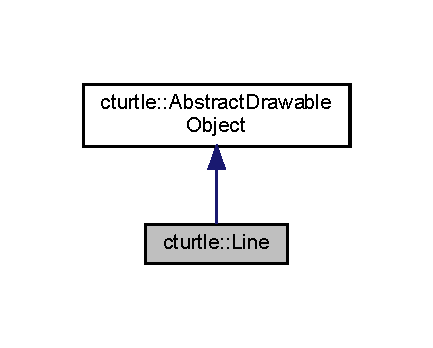
\includegraphics[width=208pt]{classcturtle_1_1Line__inherit__graph}
\end{center}
\end{figure}


Collaboration diagram for cturtle\+::Line\+:\nopagebreak
\begin{figure}[H]
\begin{center}
\leavevmode
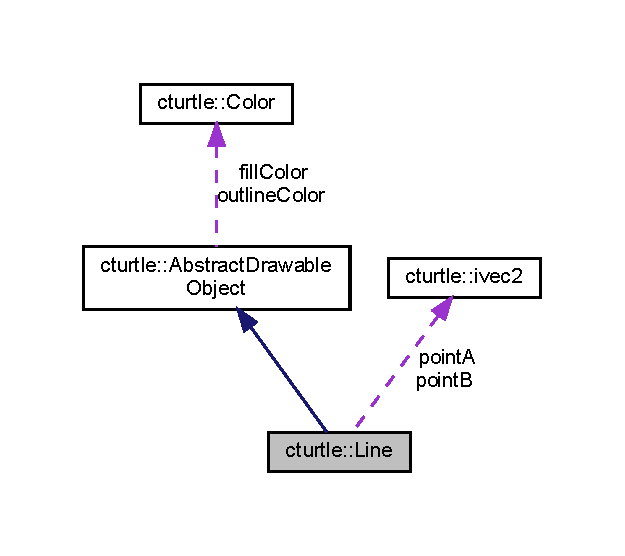
\includegraphics[width=300pt]{classcturtle_1_1Line__coll__graph}
\end{center}
\end{figure}
\doxysubsection*{Public Member Functions}
\begin{DoxyCompactItemize}
\item 
\mbox{\Hypertarget{classcturtle_1_1Line_ac6d8c8133ddbb5cafa31be364b0ed4f6}\label{classcturtle_1_1Line_ac6d8c8133ddbb5cafa31be364b0ed4f6}} 
\mbox{\hyperlink{classcturtle_1_1Line_ac6d8c8133ddbb5cafa31be364b0ed4f6}{Line}} ()
\begin{DoxyCompactList}\small\item\em Empty default constructor. \end{DoxyCompactList}\item 
\mbox{\hyperlink{classcturtle_1_1Line_ae08d302308c4b10cc714508b2acca228}{Line}} (\mbox{\hyperlink{structcturtle_1_1ivec2}{Point}} a, \mbox{\hyperlink{structcturtle_1_1ivec2}{Point}} b, \mbox{\hyperlink{classcturtle_1_1Color}{Color}} color, int \mbox{\hyperlink{classcturtle_1_1Line_ae0c426af211fc443b7ad2bed4c30050b}{width}}=1)
\begin{DoxyCompactList}\small\item\em Value constructor. merely assigns value of pointA and pointB to respective A and B. \end{DoxyCompactList}\item 
\mbox{\hyperlink{classcturtle_1_1Line_ac1b144ecd3e23c5f296b4f845f332c73}{Line}} (const \mbox{\hyperlink{classcturtle_1_1Line}{Line}} \&other)
\begin{DoxyCompactList}\small\item\em Copy constructor. Merely assigns the \char`\"{}to\char`\"{} and \char`\"{}from\char`\"{} points. \end{DoxyCompactList}\item 
\mbox{\Hypertarget{classcturtle_1_1Line_a004870caac1e5632064ff28ae5a7e0ff}\label{classcturtle_1_1Line_a004870caac1e5632064ff28ae5a7e0ff}} 
\mbox{\hyperlink{classcturtle_1_1AbstractDrawableObject}{Abstract\+Drawable\+Object}} $\ast$ \mbox{\hyperlink{classcturtle_1_1Line_a004870caac1e5632064ff28ae5a7e0ff}{copy}} () const
\begin{DoxyCompactList}\small\item\em Returns a pointer to a copy of this drawable object, allocated with N\+EW. Result Must be deleted at the responsibility of the invoker. \end{DoxyCompactList}\item 
\mbox{\Hypertarget{classcturtle_1_1Line_a885276e725f86d89f79b32ee3d885079}\label{classcturtle_1_1Line_a885276e725f86d89f79b32ee3d885079}} 
\mbox{\hyperlink{classcturtle_1_1Line_a885276e725f86d89f79b32ee3d885079}{$\sim$\+Line}} ()
\begin{DoxyCompactList}\small\item\em Empty de-\/constructor. \end{DoxyCompactList}\item 
void \mbox{\hyperlink{classcturtle_1_1Line_a25ac5b4024bf9209d324b6f8c16affaf}{draw}} (const \mbox{\hyperlink{classcturtle_1_1Transform}{Transform}} \&t, Image \&img\+Ref) const
\begin{DoxyCompactList}\small\item\em This function is intended to draw all applicable geometry in this object to the specified image, with the specified transform, with the specified color. This function is intended to be overloaded by child classes to draw applicable geometry to an image, acting as a canvas. \end{DoxyCompactList}\end{DoxyCompactItemize}
\doxysubsection*{Public Attributes}
\begin{DoxyCompactItemize}
\item 
\mbox{\hyperlink{structcturtle_1_1ivec2}{Point}} \mbox{\hyperlink{classcturtle_1_1Line_aca3d9298f4dc790552ed6515e2880ed8}{pointA}}
\item 
\mbox{\hyperlink{structcturtle_1_1ivec2}{Point}} \mbox{\hyperlink{classcturtle_1_1Line_a138b108f3a3531c4f7f72a8e26a16fcf}{pointB}}
\item 
int \mbox{\hyperlink{classcturtle_1_1Line_ae0c426af211fc443b7ad2bed4c30050b}{width}} = 1
\end{DoxyCompactItemize}


\doxysubsection{Detailed Description}
The \mbox{\hyperlink{classcturtle_1_1Line}{Line}} class holds two points and the functionality to draw a line between them on a specified canvas. 

\doxysubsection{Constructor \& Destructor Documentation}
\mbox{\Hypertarget{classcturtle_1_1Line_ae08d302308c4b10cc714508b2acca228}\label{classcturtle_1_1Line_ae08d302308c4b10cc714508b2acca228}} 
\index{cturtle::Line@{cturtle::Line}!Line@{Line}}
\index{Line@{Line}!cturtle::Line@{cturtle::Line}}
\doxysubsubsection{\texorpdfstring{Line()}{Line()}\hspace{0.1cm}{\footnotesize\ttfamily [1/2]}}
{\footnotesize\ttfamily cturtle\+::\+Line\+::\+Line (\begin{DoxyParamCaption}\item[{\mbox{\hyperlink{structcturtle_1_1ivec2}{Point}}}]{a,  }\item[{\mbox{\hyperlink{structcturtle_1_1ivec2}{Point}}}]{b,  }\item[{\mbox{\hyperlink{classcturtle_1_1Color}{Color}}}]{color,  }\item[{int}]{width = {\ttfamily 1} }\end{DoxyParamCaption})\hspace{0.3cm}{\ttfamily [inline]}}



Value constructor. merely assigns value of pointA and pointB to respective A and B. 


\begin{DoxyParams}{Parameters}
{\em a} & The \char`\"{}\+From\char`\"{} point. \\
\hline
{\em b} & The \char`\"{}\+To\char`\"{} point. \\
\hline
\end{DoxyParams}
\mbox{\Hypertarget{classcturtle_1_1Line_ac1b144ecd3e23c5f296b4f845f332c73}\label{classcturtle_1_1Line_ac1b144ecd3e23c5f296b4f845f332c73}} 
\index{cturtle::Line@{cturtle::Line}!Line@{Line}}
\index{Line@{Line}!cturtle::Line@{cturtle::Line}}
\doxysubsubsection{\texorpdfstring{Line()}{Line()}\hspace{0.1cm}{\footnotesize\ttfamily [2/2]}}
{\footnotesize\ttfamily cturtle\+::\+Line\+::\+Line (\begin{DoxyParamCaption}\item[{const \mbox{\hyperlink{classcturtle_1_1Line}{Line}} \&}]{other }\end{DoxyParamCaption})\hspace{0.3cm}{\ttfamily [inline]}}



Copy constructor. Merely assigns the \char`\"{}to\char`\"{} and \char`\"{}from\char`\"{} points. 


\begin{DoxyParams}{Parameters}
{\em other} & The other instance of a line from which to derive value. \\
\hline
\end{DoxyParams}


\doxysubsection{Member Function Documentation}
\mbox{\Hypertarget{classcturtle_1_1Line_a25ac5b4024bf9209d324b6f8c16affaf}\label{classcturtle_1_1Line_a25ac5b4024bf9209d324b6f8c16affaf}} 
\index{cturtle::Line@{cturtle::Line}!draw@{draw}}
\index{draw@{draw}!cturtle::Line@{cturtle::Line}}
\doxysubsubsection{\texorpdfstring{draw()}{draw()}}
{\footnotesize\ttfamily void cturtle\+::\+Line\+::draw (\begin{DoxyParamCaption}\item[{const \mbox{\hyperlink{classcturtle_1_1Transform}{Transform}} \&}]{t,  }\item[{Image \&}]{img\+Ref }\end{DoxyParamCaption}) const\hspace{0.3cm}{\ttfamily [inline]}, {\ttfamily [virtual]}}



This function is intended to draw all applicable geometry in this object to the specified image, with the specified transform, with the specified color. This function is intended to be overloaded by child classes to draw applicable geometry to an image, acting as a canvas. 


\begin{DoxyParams}{Parameters}
{\em t} & The transform at which to draw the geometry. \\
\hline
{\em img\+Ref} & The canvas on which to draw. \\
\hline
{\em c} & The color with to draw the geometry. \\
\hline
\end{DoxyParams}


Implements \mbox{\hyperlink{classcturtle_1_1AbstractDrawableObject_a7b1ad1e9743d343e0fe577de3978bdad}{cturtle\+::\+Abstract\+Drawable\+Object}}.



\doxysubsection{Member Data Documentation}
\mbox{\Hypertarget{classcturtle_1_1Line_aca3d9298f4dc790552ed6515e2880ed8}\label{classcturtle_1_1Line_aca3d9298f4dc790552ed6515e2880ed8}} 
\index{cturtle::Line@{cturtle::Line}!pointA@{pointA}}
\index{pointA@{pointA}!cturtle::Line@{cturtle::Line}}
\doxysubsubsection{\texorpdfstring{pointA}{pointA}}
{\footnotesize\ttfamily \mbox{\hyperlink{structcturtle_1_1ivec2}{Point}} cturtle\+::\+Line\+::pointA}

The \char`\"{}\+From\char`\"{} point. Lines drawn with this object start here. \mbox{\Hypertarget{classcturtle_1_1Line_a138b108f3a3531c4f7f72a8e26a16fcf}\label{classcturtle_1_1Line_a138b108f3a3531c4f7f72a8e26a16fcf}} 
\index{cturtle::Line@{cturtle::Line}!pointB@{pointB}}
\index{pointB@{pointB}!cturtle::Line@{cturtle::Line}}
\doxysubsubsection{\texorpdfstring{pointB}{pointB}}
{\footnotesize\ttfamily \mbox{\hyperlink{structcturtle_1_1ivec2}{Point}} cturtle\+::\+Line\+::pointB}

The \char`\"{}\+To\char`\"{} point. Lines drawn with this object end here. \mbox{\Hypertarget{classcturtle_1_1Line_ae0c426af211fc443b7ad2bed4c30050b}\label{classcturtle_1_1Line_ae0c426af211fc443b7ad2bed4c30050b}} 
\index{cturtle::Line@{cturtle::Line}!width@{width}}
\index{width@{width}!cturtle::Line@{cturtle::Line}}
\doxysubsubsection{\texorpdfstring{width}{width}}
{\footnotesize\ttfamily int cturtle\+::\+Line\+::width = 1}

The width of the line, in pixels. 

The documentation for this class was generated from the following file\+:\begin{DoxyCompactItemize}
\item 
C\+Turtle.\+hpp\end{DoxyCompactItemize}

\hypertarget{structcturtle_1_1PenState}{}\section{cturtle\+:\+:Pen\+State Struct Reference}
\label{structcturtle_1_1PenState}\index{cturtle\+::\+Pen\+State@{cturtle\+::\+Pen\+State}}


{\ttfamily \#include $<$C\+Turtle.\+hpp$>$}



Collaboration diagram for cturtle\+:\+:Pen\+State\+:
\nopagebreak
\begin{figure}[H]
\begin{center}
\leavevmode
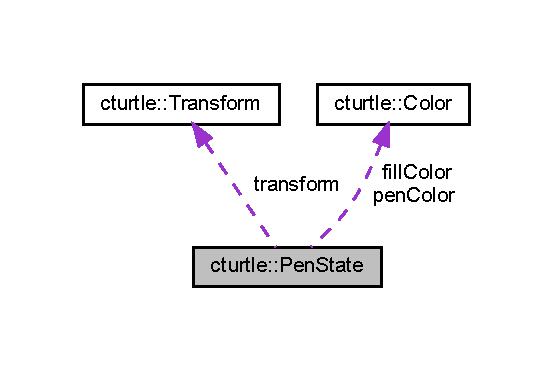
\includegraphics[width=266pt]{structcturtle_1_1PenState__coll__graph}
\end{center}
\end{figure}
\subsection*{Public Member Functions}
\begin{DoxyCompactItemize}
\item 
\mbox{\Hypertarget{structcturtle_1_1PenState_a308973ed85eee69acd4f98b72e2be21c}\label{structcturtle_1_1PenState_a308973ed85eee69acd4f98b72e2be21c}} 
{\bfseries Pen\+State} (const \hyperlink{structcturtle_1_1PenState}{Pen\+State} \&copy)
\item 
\mbox{\Hypertarget{structcturtle_1_1PenState_aa324f2f3a6cc360d8d927e677c6b6d1a}\label{structcturtle_1_1PenState_aa324f2f3a6cc360d8d927e677c6b6d1a}} 
\hyperlink{structcturtle_1_1PenState}{Pen\+State} \& {\bfseries operator=} (const \hyperlink{structcturtle_1_1PenState}{Pen\+State} \&copy)
\end{DoxyCompactItemize}
\subsection*{Public Attributes}
\begin{DoxyCompactItemize}
\item 
\hyperlink{classcturtle_1_1Transform}{Transform} \hyperlink{structcturtle_1_1PenState_ac6b3e58155d09bf78a315c616874fa89}{transform}
\item 
float \hyperlink{structcturtle_1_1PenState_af5432bc75dcc374e6269a28a656a6c49}{move\+Speed} = T\+S\+\_\+\+N\+O\+R\+M\+AL
\item 
bool \hyperlink{structcturtle_1_1PenState_aa6992297fb8f109e20599c31dd29cd6f}{tracing} = true
\item 
bool \hyperlink{structcturtle_1_1PenState_ae860bb135dc50937453694b8331a014d}{angle\+Mode} = false
\item 
int \hyperlink{structcturtle_1_1PenState_a5ca3f05c53ca672de4466e4c7f5f3328}{pen\+Width} = 1
\item 
bool \hyperlink{structcturtle_1_1PenState_aa74bc9fbcc2f4eba76d8b8856ba30eff}{filling} = false
\item 
\hyperlink{classcturtle_1_1Color}{Color} \hyperlink{structcturtle_1_1PenState_a2fb76e7573bfa387e1858df701dab60b}{pen\+Color} = \hyperlink{classcturtle_1_1Color}{Color}(\char`\"{}black\char`\"{})
\item 
\hyperlink{classcturtle_1_1Color}{Color} \hyperlink{structcturtle_1_1PenState_a787b9819a36fe8b87d7ce60574df19df}{fill\+Color} = \hyperlink{classcturtle_1_1Color}{Color}(\char`\"{}black\char`\"{})
\item 
size\+\_\+t \hyperlink{structcturtle_1_1PenState_a7309ce91cbc711775e59a9ce1ed150a5}{objects\+Before} = 0
\item 
std\+::unique\+\_\+ptr$<$ \hyperlink{classcturtle_1_1AbstractDrawableObject}{Abstract\+Drawable\+Object} $>$ \hyperlink{structcturtle_1_1PenState_af57060055c671d34395271a50553b922}{cursor} = nullptr
\item 
int \hyperlink{structcturtle_1_1PenState_a5a5c623893c76f00325223e075af714b}{cur\+Stamp} = 0
\item 
bool \hyperlink{structcturtle_1_1PenState_a7c1380e85858e04607427fcddeb1cba7}{visible} = true
\item 
float \hyperlink{structcturtle_1_1PenState_a6ebb8d220523e19a27922ff5d04931de}{cursor\+Tilt} = 0
\end{DoxyCompactItemize}


\subsection{Detailed Description}
Pen State structure. Holds all pen attributes. 

\subsection{Member Data Documentation}
\mbox{\Hypertarget{structcturtle_1_1PenState_ae860bb135dc50937453694b8331a014d}\label{structcturtle_1_1PenState_ae860bb135dc50937453694b8331a014d}} 
\index{cturtle\+::\+Pen\+State@{cturtle\+::\+Pen\+State}!angle\+Mode@{angle\+Mode}}
\index{angle\+Mode@{angle\+Mode}!cturtle\+::\+Pen\+State@{cturtle\+::\+Pen\+State}}
\subsubsection{\texorpdfstring{angle\+Mode}{angleMode}}
{\footnotesize\ttfamily bool cturtle\+::\+Pen\+State\+::angle\+Mode = false}

The angle mode. False for degrees, true for radians. \mbox{\Hypertarget{structcturtle_1_1PenState_af57060055c671d34395271a50553b922}\label{structcturtle_1_1PenState_af57060055c671d34395271a50553b922}} 
\index{cturtle\+::\+Pen\+State@{cturtle\+::\+Pen\+State}!cursor@{cursor}}
\index{cursor@{cursor}!cturtle\+::\+Pen\+State@{cturtle\+::\+Pen\+State}}
\subsubsection{\texorpdfstring{cursor}{cursor}}
{\footnotesize\ttfamily std\+::unique\+\_\+ptr$<$\hyperlink{classcturtle_1_1AbstractDrawableObject}{Abstract\+Drawable\+Object}$>$ cturtle\+::\+Pen\+State\+::cursor = nullptr}

The turtle\textquotesingle{}s cursor geometry. M\+U\+ST A\+S\+S\+I\+GN B\+E\+F\+O\+RE U\+SE. \mbox{\Hypertarget{structcturtle_1_1PenState_a6ebb8d220523e19a27922ff5d04931de}\label{structcturtle_1_1PenState_a6ebb8d220523e19a27922ff5d04931de}} 
\index{cturtle\+::\+Pen\+State@{cturtle\+::\+Pen\+State}!cursor\+Tilt@{cursor\+Tilt}}
\index{cursor\+Tilt@{cursor\+Tilt}!cturtle\+::\+Pen\+State@{cturtle\+::\+Pen\+State}}
\subsubsection{\texorpdfstring{cursor\+Tilt}{cursorTilt}}
{\footnotesize\ttfamily float cturtle\+::\+Pen\+State\+::cursor\+Tilt = 0}

A float for cursor tilt (e.\+g, rotation appleid to the cursor itself) \mbox{\Hypertarget{structcturtle_1_1PenState_a5a5c623893c76f00325223e075af714b}\label{structcturtle_1_1PenState_a5a5c623893c76f00325223e075af714b}} 
\index{cturtle\+::\+Pen\+State@{cturtle\+::\+Pen\+State}!cur\+Stamp@{cur\+Stamp}}
\index{cur\+Stamp@{cur\+Stamp}!cturtle\+::\+Pen\+State@{cturtle\+::\+Pen\+State}}
\subsubsection{\texorpdfstring{cur\+Stamp}{curStamp}}
{\footnotesize\ttfamily int cturtle\+::\+Pen\+State\+::cur\+Stamp = 0}

The current stamp ID. \mbox{\Hypertarget{structcturtle_1_1PenState_a787b9819a36fe8b87d7ce60574df19df}\label{structcturtle_1_1PenState_a787b9819a36fe8b87d7ce60574df19df}} 
\index{cturtle\+::\+Pen\+State@{cturtle\+::\+Pen\+State}!fill\+Color@{fill\+Color}}
\index{fill\+Color@{fill\+Color}!cturtle\+::\+Pen\+State@{cturtle\+::\+Pen\+State}}
\subsubsection{\texorpdfstring{fill\+Color}{fillColor}}
{\footnotesize\ttfamily \hyperlink{classcturtle_1_1Color}{Color} cturtle\+::\+Pen\+State\+::fill\+Color = \hyperlink{classcturtle_1_1Color}{Color}(\char`\"{}black\char`\"{})}

The intended fill color. \mbox{\Hypertarget{structcturtle_1_1PenState_aa74bc9fbcc2f4eba76d8b8856ba30eff}\label{structcturtle_1_1PenState_aa74bc9fbcc2f4eba76d8b8856ba30eff}} 
\index{cturtle\+::\+Pen\+State@{cturtle\+::\+Pen\+State}!filling@{filling}}
\index{filling@{filling}!cturtle\+::\+Pen\+State@{cturtle\+::\+Pen\+State}}
\subsubsection{\texorpdfstring{filling}{filling}}
{\footnotesize\ttfamily bool cturtle\+::\+Pen\+State\+::filling = false}

A boolean indicating if we\textquotesingle{}re trying to fill a shape. \mbox{\Hypertarget{structcturtle_1_1PenState_af5432bc75dcc374e6269a28a656a6c49}\label{structcturtle_1_1PenState_af5432bc75dcc374e6269a28a656a6c49}} 
\index{cturtle\+::\+Pen\+State@{cturtle\+::\+Pen\+State}!move\+Speed@{move\+Speed}}
\index{move\+Speed@{move\+Speed}!cturtle\+::\+Pen\+State@{cturtle\+::\+Pen\+State}}
\subsubsection{\texorpdfstring{move\+Speed}{moveSpeed}}
{\footnotesize\ttfamily float cturtle\+::\+Pen\+State\+::move\+Speed = T\+S\+\_\+\+N\+O\+R\+M\+AL}

The movement speed of the turtle, in range of 0...10 \mbox{\Hypertarget{structcturtle_1_1PenState_a7309ce91cbc711775e59a9ce1ed150a5}\label{structcturtle_1_1PenState_a7309ce91cbc711775e59a9ce1ed150a5}} 
\index{cturtle\+::\+Pen\+State@{cturtle\+::\+Pen\+State}!objects\+Before@{objects\+Before}}
\index{objects\+Before@{objects\+Before}!cturtle\+::\+Pen\+State@{cturtle\+::\+Pen\+State}}
\subsubsection{\texorpdfstring{objects\+Before}{objectsBefore}}
{\footnotesize\ttfamily size\+\_\+t cturtle\+::\+Pen\+State\+::objects\+Before = 0}

The total number of objects in the screen\textquotesingle{}s object stack prior to the addition of this state-\/$>$ \mbox{\Hypertarget{structcturtle_1_1PenState_a2fb76e7573bfa387e1858df701dab60b}\label{structcturtle_1_1PenState_a2fb76e7573bfa387e1858df701dab60b}} 
\index{cturtle\+::\+Pen\+State@{cturtle\+::\+Pen\+State}!pen\+Color@{pen\+Color}}
\index{pen\+Color@{pen\+Color}!cturtle\+::\+Pen\+State@{cturtle\+::\+Pen\+State}}
\subsubsection{\texorpdfstring{pen\+Color}{penColor}}
{\footnotesize\ttfamily \hyperlink{classcturtle_1_1Color}{Color} cturtle\+::\+Pen\+State\+::pen\+Color = \hyperlink{classcturtle_1_1Color}{Color}(\char`\"{}black\char`\"{})}

The color of the pen. \mbox{\Hypertarget{structcturtle_1_1PenState_a5ca3f05c53ca672de4466e4c7f5f3328}\label{structcturtle_1_1PenState_a5ca3f05c53ca672de4466e4c7f5f3328}} 
\index{cturtle\+::\+Pen\+State@{cturtle\+::\+Pen\+State}!pen\+Width@{pen\+Width}}
\index{pen\+Width@{pen\+Width}!cturtle\+::\+Pen\+State@{cturtle\+::\+Pen\+State}}
\subsubsection{\texorpdfstring{pen\+Width}{penWidth}}
{\footnotesize\ttfamily int cturtle\+::\+Pen\+State\+::pen\+Width = 1}

The width of the pen, in pixels. \mbox{\Hypertarget{structcturtle_1_1PenState_aa6992297fb8f109e20599c31dd29cd6f}\label{structcturtle_1_1PenState_aa6992297fb8f109e20599c31dd29cd6f}} 
\index{cturtle\+::\+Pen\+State@{cturtle\+::\+Pen\+State}!tracing@{tracing}}
\index{tracing@{tracing}!cturtle\+::\+Pen\+State@{cturtle\+::\+Pen\+State}}
\subsubsection{\texorpdfstring{tracing}{tracing}}
{\footnotesize\ttfamily bool cturtle\+::\+Pen\+State\+::tracing = true}

Whether or not the turtle\textquotesingle{}s \char`\"{}tail\char`\"{} (or pen) is down. \mbox{\Hypertarget{structcturtle_1_1PenState_ac6b3e58155d09bf78a315c616874fa89}\label{structcturtle_1_1PenState_ac6b3e58155d09bf78a315c616874fa89}} 
\index{cturtle\+::\+Pen\+State@{cturtle\+::\+Pen\+State}!transform@{transform}}
\index{transform@{transform}!cturtle\+::\+Pen\+State@{cturtle\+::\+Pen\+State}}
\subsubsection{\texorpdfstring{transform}{transform}}
{\footnotesize\ttfamily \hyperlink{classcturtle_1_1Transform}{Transform} cturtle\+::\+Pen\+State\+::transform}

The transform of the pen. holds position, rotation, and scale of the turtle. \mbox{\Hypertarget{structcturtle_1_1PenState_a7c1380e85858e04607427fcddeb1cba7}\label{structcturtle_1_1PenState_a7c1380e85858e04607427fcddeb1cba7}} 
\index{cturtle\+::\+Pen\+State@{cturtle\+::\+Pen\+State}!visible@{visible}}
\index{visible@{visible}!cturtle\+::\+Pen\+State@{cturtle\+::\+Pen\+State}}
\subsubsection{\texorpdfstring{visible}{visible}}
{\footnotesize\ttfamily bool cturtle\+::\+Pen\+State\+::visible = true}

A boolean indicating if this turtle is visible. 

The documentation for this struct was generated from the following file\+:\begin{DoxyCompactItemize}
\item 
C\+Turtle.\+hpp\end{DoxyCompactItemize}

\hypertarget{classcturtle_1_1Polygon}{}\doxysection{cturtle\+::Polygon Class Reference}
\label{classcturtle_1_1Polygon}\index{cturtle::Polygon@{cturtle::Polygon}}


The polygon class merely holds a vector of points and a function to draw this series to an image. Please note that the contained series of points must be in either clockwise(\+CW) or counterclockwise(\+CCW) order!  




{\ttfamily \#include $<$CTurtle.\+hpp$>$}



Inheritance diagram for cturtle\+::Polygon\+:\nopagebreak
\begin{figure}[H]
\begin{center}
\leavevmode
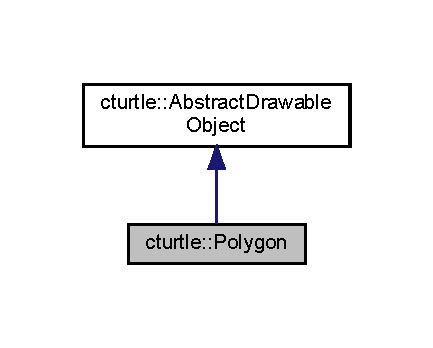
\includegraphics[width=208pt]{classcturtle_1_1Polygon__inherit__graph}
\end{center}
\end{figure}


Collaboration diagram for cturtle\+::Polygon\+:\nopagebreak
\begin{figure}[H]
\begin{center}
\leavevmode
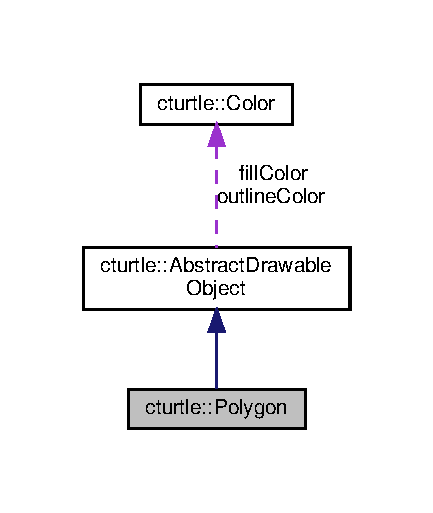
\includegraphics[width=208pt]{classcturtle_1_1Polygon__coll__graph}
\end{center}
\end{figure}
\doxysubsection*{Public Member Functions}
\begin{DoxyCompactItemize}
\item 
\mbox{\Hypertarget{classcturtle_1_1Polygon_a2e345458c2770bd889756d0c2f7f193e}\label{classcturtle_1_1Polygon_a2e345458c2770bd889756d0c2f7f193e}} 
\mbox{\hyperlink{classcturtle_1_1Polygon_a2e345458c2770bd889756d0c2f7f193e}{Polygon}} ()=default
\begin{DoxyCompactList}\small\item\em Empty default constructor. \end{DoxyCompactList}\item 
\mbox{\hyperlink{classcturtle_1_1Polygon_a035f78fca7139d12bc9626105bc326e3}{Polygon}} (const std\+::initializer\+\_\+list$<$ \mbox{\hyperlink{structcturtle_1_1ivec2}{Point}} $>$ \&init)
\begin{DoxyCompactList}\small\item\em Initializer list instructor which assigns the points to the contents of the specified initializer list. \end{DoxyCompactList}\item 
\mbox{\hyperlink{classcturtle_1_1Polygon_a5c884cfe0c0f595403ccb3864b85893a}{Polygon}} (std\+::vector$<$ \mbox{\hyperlink{structcturtle_1_1ivec2}{Point}} $>$ \mbox{\hyperlink{classcturtle_1_1Polygon_a6af3a67289f39af96fe704e75a2828c9}{copy}}, const \mbox{\hyperlink{classcturtle_1_1Color}{Color}} \&\mbox{\hyperlink{classcturtle_1_1AbstractDrawableObject_a37d635a02ad3e5206a6eb99b7b5f1963}{fill\+Color}}, int \mbox{\hyperlink{classcturtle_1_1AbstractDrawableObject_aeffaecc245057e9a42e5688671a77f52}{outline\+Width}}=0, const \mbox{\hyperlink{classcturtle_1_1Color}{Color}} \&\mbox{\hyperlink{classcturtle_1_1AbstractDrawableObject_abd04640855e7623bb84b52babd8b32b6}{outline\+Color}}=\mbox{\hyperlink{classcturtle_1_1Color}{Color}}())
\begin{DoxyCompactList}\small\item\em A copy constructor for another vector of points. \end{DoxyCompactList}\item 
\mbox{\hyperlink{classcturtle_1_1Polygon_aadcd2d6cbfd953a6062724c3370dc08c}{Polygon}} (const \mbox{\hyperlink{classcturtle_1_1Polygon}{Polygon}} \&other)=default
\begin{DoxyCompactList}\small\item\em A copy constructor for another polygon. \end{DoxyCompactList}\item 
\mbox{\hyperlink{classcturtle_1_1AbstractDrawableObject}{Abstract\+Drawable\+Object}} $\ast$ \mbox{\hyperlink{classcturtle_1_1Polygon_a6af3a67289f39af96fe704e75a2828c9}{copy}} () const override
\item 
\mbox{\Hypertarget{classcturtle_1_1Polygon_a0ce8b8aa4b195b11d13be873856349f7}\label{classcturtle_1_1Polygon_a0ce8b8aa4b195b11d13be873856349f7}} 
\mbox{\hyperlink{classcturtle_1_1Polygon_a0ce8b8aa4b195b11d13be873856349f7}{$\sim$\+Polygon}} () override=default
\begin{DoxyCompactList}\small\item\em Empty de-\/constructor. \end{DoxyCompactList}\item 
void \mbox{\hyperlink{classcturtle_1_1Polygon_afb7ae3ca0a862f9f0aa1c1720a5d40a6}{draw}} (const \mbox{\hyperlink{classcturtle_1_1Transform}{Transform}} \&t, Image \&img\+Ref) const override
\begin{DoxyCompactList}\small\item\em This function is intended to draw all applicable geometry in this object to the specified image, with the specified transform, with the specified color. This function is intended to be overloaded by child classes to draw applicable geometry to an image, acting as a canvas. \end{DoxyCompactList}\end{DoxyCompactItemize}
\doxysubsection*{Public Attributes}
\begin{DoxyCompactItemize}
\item 
\mbox{\Hypertarget{classcturtle_1_1Polygon_a384a2dba19b3181382c6d40c1c374cfe}\label{classcturtle_1_1Polygon_a384a2dba19b3181382c6d40c1c374cfe}} 
std\+::vector$<$ \mbox{\hyperlink{structcturtle_1_1ivec2}{Point}} $>$ {\bfseries points}
\end{DoxyCompactItemize}
\doxysubsection*{Additional Inherited Members}


\doxysubsection{Detailed Description}
The polygon class merely holds a vector of points and a function to draw this series to an image. Please note that the contained series of points must be in either clockwise(\+CW) or counterclockwise(\+CCW) order! 

\doxysubsection{Constructor \& Destructor Documentation}
\mbox{\Hypertarget{classcturtle_1_1Polygon_a035f78fca7139d12bc9626105bc326e3}\label{classcturtle_1_1Polygon_a035f78fca7139d12bc9626105bc326e3}} 
\index{cturtle::Polygon@{cturtle::Polygon}!Polygon@{Polygon}}
\index{Polygon@{Polygon}!cturtle::Polygon@{cturtle::Polygon}}
\doxysubsubsection{\texorpdfstring{Polygon()}{Polygon()}\hspace{0.1cm}{\footnotesize\ttfamily [1/3]}}
{\footnotesize\ttfamily cturtle\+::\+Polygon\+::\+Polygon (\begin{DoxyParamCaption}\item[{const std\+::initializer\+\_\+list$<$ \mbox{\hyperlink{structcturtle_1_1ivec2}{Point}} $>$ \&}]{init }\end{DoxyParamCaption})\hspace{0.3cm}{\ttfamily [inline]}}



Initializer list instructor which assigns the points to the contents of the specified initializer list. 


\begin{DoxyParams}{Parameters}
{\em The} & initializer list from where points are retrieved. \\
\hline
\end{DoxyParams}
\mbox{\Hypertarget{classcturtle_1_1Polygon_a5c884cfe0c0f595403ccb3864b85893a}\label{classcturtle_1_1Polygon_a5c884cfe0c0f595403ccb3864b85893a}} 
\index{cturtle::Polygon@{cturtle::Polygon}!Polygon@{Polygon}}
\index{Polygon@{Polygon}!cturtle::Polygon@{cturtle::Polygon}}
\doxysubsubsection{\texorpdfstring{Polygon()}{Polygon()}\hspace{0.1cm}{\footnotesize\ttfamily [2/3]}}
{\footnotesize\ttfamily cturtle\+::\+Polygon\+::\+Polygon (\begin{DoxyParamCaption}\item[{std\+::vector$<$ \mbox{\hyperlink{structcturtle_1_1ivec2}{Point}} $>$}]{copy,  }\item[{const \mbox{\hyperlink{classcturtle_1_1Color}{Color}} \&}]{fill\+Color,  }\item[{int}]{outline\+Width = {\ttfamily 0},  }\item[{const \mbox{\hyperlink{classcturtle_1_1Color}{Color}} \&}]{outline\+Color = {\ttfamily \mbox{\hyperlink{classcturtle_1_1Color}{Color}}()} }\end{DoxyParamCaption})\hspace{0.3cm}{\ttfamily [inline]}}



A copy constructor for another vector of points. 


\begin{DoxyParams}{Parameters}
{\em copy} & A vector from which to derive points. \\
\hline
\end{DoxyParams}
\mbox{\Hypertarget{classcturtle_1_1Polygon_aadcd2d6cbfd953a6062724c3370dc08c}\label{classcturtle_1_1Polygon_aadcd2d6cbfd953a6062724c3370dc08c}} 
\index{cturtle::Polygon@{cturtle::Polygon}!Polygon@{Polygon}}
\index{Polygon@{Polygon}!cturtle::Polygon@{cturtle::Polygon}}
\doxysubsubsection{\texorpdfstring{Polygon()}{Polygon()}\hspace{0.1cm}{\footnotesize\ttfamily [3/3]}}
{\footnotesize\ttfamily cturtle\+::\+Polygon\+::\+Polygon (\begin{DoxyParamCaption}\item[{const \mbox{\hyperlink{classcturtle_1_1Polygon}{Polygon}} \&}]{other }\end{DoxyParamCaption})\hspace{0.3cm}{\ttfamily [default]}}



A copy constructor for another polygon. 


\begin{DoxyParams}{Parameters}
{\em other} & Another polygon from which to derive points. \\
\hline
\end{DoxyParams}


\doxysubsection{Member Function Documentation}
\mbox{\Hypertarget{classcturtle_1_1Polygon_a6af3a67289f39af96fe704e75a2828c9}\label{classcturtle_1_1Polygon_a6af3a67289f39af96fe704e75a2828c9}} 
\index{cturtle::Polygon@{cturtle::Polygon}!copy@{copy}}
\index{copy@{copy}!cturtle::Polygon@{cturtle::Polygon}}
\doxysubsubsection{\texorpdfstring{copy()}{copy()}}
{\footnotesize\ttfamily \mbox{\hyperlink{classcturtle_1_1AbstractDrawableObject}{Abstract\+Drawable\+Object}}$\ast$ cturtle\+::\+Polygon\+::copy (\begin{DoxyParamCaption}{ }\end{DoxyParamCaption}) const\hspace{0.3cm}{\ttfamily [inline]}, {\ttfamily [override]}, {\ttfamily [virtual]}}

Returns a copy of this polygon allocated with the new keyword. Must be deleted at the responsibility of the invoker. 

Implements \mbox{\hyperlink{classcturtle_1_1AbstractDrawableObject_acff3437e999d281773b66e6cf2115372}{cturtle\+::\+Abstract\+Drawable\+Object}}.

\mbox{\Hypertarget{classcturtle_1_1Polygon_afb7ae3ca0a862f9f0aa1c1720a5d40a6}\label{classcturtle_1_1Polygon_afb7ae3ca0a862f9f0aa1c1720a5d40a6}} 
\index{cturtle::Polygon@{cturtle::Polygon}!draw@{draw}}
\index{draw@{draw}!cturtle::Polygon@{cturtle::Polygon}}
\doxysubsubsection{\texorpdfstring{draw()}{draw()}}
{\footnotesize\ttfamily void cturtle\+::\+Polygon\+::draw (\begin{DoxyParamCaption}\item[{const \mbox{\hyperlink{classcturtle_1_1Transform}{Transform}} \&}]{t,  }\item[{Image \&}]{img\+Ref }\end{DoxyParamCaption}) const\hspace{0.3cm}{\ttfamily [inline]}, {\ttfamily [override]}, {\ttfamily [virtual]}}



This function is intended to draw all applicable geometry in this object to the specified image, with the specified transform, with the specified color. This function is intended to be overloaded by child classes to draw applicable geometry to an image, acting as a canvas. 


\begin{DoxyParams}{Parameters}
{\em t} & The transform at which to draw the geometry. \\
\hline
{\em img\+Ref} & The canvas on which to draw. \\
\hline
{\em c} & The color with to draw the geometry. \\
\hline
\end{DoxyParams}


Implements \mbox{\hyperlink{classcturtle_1_1AbstractDrawableObject_a7b1ad1e9743d343e0fe577de3978bdad}{cturtle\+::\+Abstract\+Drawable\+Object}}.



The documentation for this class was generated from the following file\+:\begin{DoxyCompactItemize}
\item 
CTurtle.\+hpp\end{DoxyCompactItemize}

\hypertarget{structcturtle_1_1SceneObject}{}\section{cturtle\+:\+:Scene\+Object Struct Reference}
\label{structcturtle_1_1SceneObject}\index{cturtle\+::\+Scene\+Object@{cturtle\+::\+Scene\+Object}}


Turtles append Scene Objects to a list to keep track of what it has drawn (a history). \hyperlink{structcturtle_1_1SceneObject}{Scene\+Object} holds a description of something that needs to be on the screen. It\textquotesingle{}s a general object which encompasses A\+LL things that can be on screen, ranging from stamps, misc. geometry, and strings.  




{\ttfamily \#include $<$C\+Turtle.\+hpp$>$}



Collaboration diagram for cturtle\+:\+:Scene\+Object\+:
\nopagebreak
\begin{figure}[H]
\begin{center}
\leavevmode
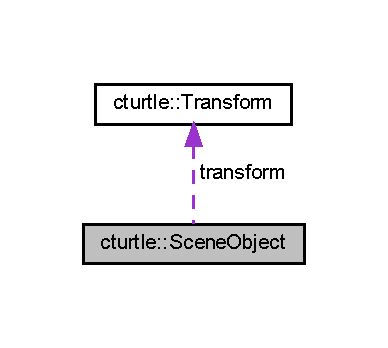
\includegraphics[width=186pt]{structcturtle_1_1SceneObject__coll__graph}
\end{center}
\end{figure}
\subsection*{Public Member Functions}
\begin{DoxyCompactItemize}
\item 
\hyperlink{structcturtle_1_1SceneObject_ac51b04f4e0509e37a7acce739e608e49}{Scene\+Object} ()
\item 
\hyperlink{structcturtle_1_1SceneObject_a278686eef9384bed5d891065a3a02619}{Scene\+Object} (\hyperlink{classcturtle_1_1AbstractDrawableObject}{Abstract\+Drawable\+Object} $\ast$\hyperlink{structcturtle_1_1SceneObject_a1db44363183fd197b232d5f6e4b89b5c}{geom}, const \hyperlink{classcturtle_1_1Transform}{Transform} \&t, int \hyperlink{structcturtle_1_1SceneObject_ae6094918613e5d4d284805cd5afb2e65}{stampid}=-\/1)
\end{DoxyCompactItemize}
\subsection*{Public Attributes}
\begin{DoxyCompactItemize}
\item 
std\+::unique\+\_\+ptr$<$ \hyperlink{classcturtle_1_1AbstractDrawableObject}{Abstract\+Drawable\+Object} $>$ \hyperlink{structcturtle_1_1SceneObject_a1db44363183fd197b232d5f6e4b89b5c}{geom}
\item 
\hyperlink{classcturtle_1_1Transform}{Transform} \hyperlink{structcturtle_1_1SceneObject_a427fb0ab63fa9e0dd5c7b5c15ac3f6f4}{transform}
\item 
bool \hyperlink{structcturtle_1_1SceneObject_a014644aee0792d77bd84a0b98464f39b}{stamp} = false
\item 
int \hyperlink{structcturtle_1_1SceneObject_ae6094918613e5d4d284805cd5afb2e65}{stampid} = -\/1
\end{DoxyCompactItemize}


\subsection{Detailed Description}
Turtles append Scene Objects to a list to keep track of what it has drawn (a history). \hyperlink{structcturtle_1_1SceneObject}{Scene\+Object} holds a description of something that needs to be on the screen. It\textquotesingle{}s a general object which encompasses A\+LL things that can be on screen, ranging from stamps, misc. geometry, and strings. 

\subsection{Constructor \& Destructor Documentation}
\mbox{\Hypertarget{structcturtle_1_1SceneObject_ac51b04f4e0509e37a7acce739e608e49}\label{structcturtle_1_1SceneObject_ac51b04f4e0509e37a7acce739e608e49}} 
\index{cturtle\+::\+Scene\+Object@{cturtle\+::\+Scene\+Object}!Scene\+Object@{Scene\+Object}}
\index{Scene\+Object@{Scene\+Object}!cturtle\+::\+Scene\+Object@{cturtle\+::\+Scene\+Object}}
\subsubsection{\texorpdfstring{Scene\+Object()}{SceneObject()}\hspace{0.1cm}{\footnotesize\ttfamily [1/2]}}
{\footnotesize\ttfamily cturtle\+::\+Scene\+Object\+::\+Scene\+Object (\begin{DoxyParamCaption}{ }\end{DoxyParamCaption})\hspace{0.3cm}{\ttfamily [inline]}}

Empty constructor. \mbox{\Hypertarget{structcturtle_1_1SceneObject_a278686eef9384bed5d891065a3a02619}\label{structcturtle_1_1SceneObject_a278686eef9384bed5d891065a3a02619}} 
\index{cturtle\+::\+Scene\+Object@{cturtle\+::\+Scene\+Object}!Scene\+Object@{Scene\+Object}}
\index{Scene\+Object@{Scene\+Object}!cturtle\+::\+Scene\+Object@{cturtle\+::\+Scene\+Object}}
\subsubsection{\texorpdfstring{Scene\+Object()}{SceneObject()}\hspace{0.1cm}{\footnotesize\ttfamily [2/2]}}
{\footnotesize\ttfamily cturtle\+::\+Scene\+Object\+::\+Scene\+Object (\begin{DoxyParamCaption}\item[{\hyperlink{classcturtle_1_1AbstractDrawableObject}{Abstract\+Drawable\+Object} $\ast$}]{geom,  }\item[{const \hyperlink{classcturtle_1_1Transform}{Transform} \&}]{t,  }\item[{int}]{stampid = {\ttfamily -\/1} }\end{DoxyParamCaption})\hspace{0.3cm}{\ttfamily [inline]}}

General geometry constructor. 
\begin{DoxyParams}{Parameters}
{\em geom} & A dynamically allocated pointer to a Geometry object. Please note that, after this constructor call, the \hyperlink{structcturtle_1_1SceneObject}{Scene\+Object} controls the life of the given pointer. Do not delete it yourself. \\
\hline
{\em color} & The color to draw the geometry in. \\
\hline
{\em t} & The transform at which to draw the geometry. \\
\hline
{\em stampid} & The ID of the stamp this object is related to. \\
\hline
\end{DoxyParams}


\subsection{Member Data Documentation}
\mbox{\Hypertarget{structcturtle_1_1SceneObject_a1db44363183fd197b232d5f6e4b89b5c}\label{structcturtle_1_1SceneObject_a1db44363183fd197b232d5f6e4b89b5c}} 
\index{cturtle\+::\+Scene\+Object@{cturtle\+::\+Scene\+Object}!geom@{geom}}
\index{geom@{geom}!cturtle\+::\+Scene\+Object@{cturtle\+::\+Scene\+Object}}
\subsubsection{\texorpdfstring{geom}{geom}}
{\footnotesize\ttfamily std\+::unique\+\_\+ptr$<$\hyperlink{classcturtle_1_1AbstractDrawableObject}{Abstract\+Drawable\+Object}$>$ cturtle\+::\+Scene\+Object\+::geom}

The unique pointer to the geometry of this object. M\+U\+ST BE N\+O\+N-\/\+N\+U\+LL IF T\+HE O\+B\+J\+E\+CT IS IN A T\+U\+R\+T\+LE S\+C\+R\+E\+EN\textquotesingle{}S S\+C\+E\+NE. \mbox{\Hypertarget{structcturtle_1_1SceneObject_a014644aee0792d77bd84a0b98464f39b}\label{structcturtle_1_1SceneObject_a014644aee0792d77bd84a0b98464f39b}} 
\index{cturtle\+::\+Scene\+Object@{cturtle\+::\+Scene\+Object}!stamp@{stamp}}
\index{stamp@{stamp}!cturtle\+::\+Scene\+Object@{cturtle\+::\+Scene\+Object}}
\subsubsection{\texorpdfstring{stamp}{stamp}}
{\footnotesize\ttfamily bool cturtle\+::\+Scene\+Object\+::stamp = false}

A boolean indicating if this scene object is a stamp. \mbox{\Hypertarget{structcturtle_1_1SceneObject_ae6094918613e5d4d284805cd5afb2e65}\label{structcturtle_1_1SceneObject_ae6094918613e5d4d284805cd5afb2e65}} 
\index{cturtle\+::\+Scene\+Object@{cturtle\+::\+Scene\+Object}!stampid@{stampid}}
\index{stampid@{stampid}!cturtle\+::\+Scene\+Object@{cturtle\+::\+Scene\+Object}}
\subsubsection{\texorpdfstring{stampid}{stampid}}
{\footnotesize\ttfamily int cturtle\+::\+Scene\+Object\+::stampid = -\/1}

The integer representing the stamp ID, if this is a stamp. Valid stampids $>$ -\/1 \mbox{\Hypertarget{structcturtle_1_1SceneObject_a427fb0ab63fa9e0dd5c7b5c15ac3f6f4}\label{structcturtle_1_1SceneObject_a427fb0ab63fa9e0dd5c7b5c15ac3f6f4}} 
\index{cturtle\+::\+Scene\+Object@{cturtle\+::\+Scene\+Object}!transform@{transform}}
\index{transform@{transform}!cturtle\+::\+Scene\+Object@{cturtle\+::\+Scene\+Object}}
\subsubsection{\texorpdfstring{transform}{transform}}
{\footnotesize\ttfamily \hyperlink{classcturtle_1_1Transform}{Transform} cturtle\+::\+Scene\+Object\+::transform}

The transform at which to draw this \hyperlink{structcturtle_1_1SceneObject}{Scene\+Object}. Note that this is concatenated onto the Screen\+Transform of the drawing turtle\textquotesingle{}s screen. 

The documentation for this struct was generated from the following file\+:\begin{DoxyCompactItemize}
\item 
C\+Turtle.\+hpp\end{DoxyCompactItemize}

\hypertarget{classcturtle_1_1Sprite}{}\section{cturtle\+:\+:Sprite Class Reference}
\label{classcturtle_1_1Sprite}\index{cturtle\+::\+Sprite@{cturtle\+::\+Sprite}}


{\ttfamily \#include $<$C\+Turtle.\+hpp$>$}



Inheritance diagram for cturtle\+:\+:Sprite\+:
% FIG 0


Collaboration diagram for cturtle\+:\+:Sprite\+:
% FIG 1
\subsection*{Public Member Functions}
\begin{DoxyCompactItemize}
\item 
\mbox{\Hypertarget{classcturtle_1_1Sprite_adca3803189c23c887a3f39de00db4bdd}\label{classcturtle_1_1Sprite_adca3803189c23c887a3f39de00db4bdd}} 
{\bfseries Sprite} (Image \&img, int \hyperlink{classcturtle_1_1AbstractDrawableObject_aeffaecc245057e9a42e5688671a77f52}{outline\+Width}=0, \hyperlink{classcturtle_1_1Color}{Color} \hyperlink{classcturtle_1_1AbstractDrawableObject_abd04640855e7623bb84b52babd8b32b6}{outline\+Color}=\hyperlink{classcturtle_1_1Color}{Color}())
\item 
\mbox{\Hypertarget{classcturtle_1_1Sprite_a56cdc4cb92ae5a5108cb34c9c284ebb0}\label{classcturtle_1_1Sprite_a56cdc4cb92ae5a5108cb34c9c284ebb0}} 
{\bfseries Sprite} (Image \&img, int srcX, int srcY, int srcW, int srcH, int \hyperlink{classcturtle_1_1AbstractDrawableObject_aeffaecc245057e9a42e5688671a77f52}{outline\+Width}=0, \hyperlink{classcturtle_1_1Color}{Color} \hyperlink{classcturtle_1_1AbstractDrawableObject_abd04640855e7623bb84b52babd8b32b6}{outline\+Color}=\hyperlink{classcturtle_1_1Color}{Color}())
\item 
\mbox{\Hypertarget{classcturtle_1_1Sprite_a818e253f4d3cbb268e753f5ceee12d1d}\label{classcturtle_1_1Sprite_a818e253f4d3cbb268e753f5ceee12d1d}} 
{\bfseries Sprite} (const \hyperlink{classcturtle_1_1Sprite}{Sprite} \&\hyperlink{classcturtle_1_1Sprite_a96682206c9ba4d31e73526d657fd346b}{copy})
\item 
\mbox{\Hypertarget{classcturtle_1_1Sprite_a96682206c9ba4d31e73526d657fd346b}\label{classcturtle_1_1Sprite_a96682206c9ba4d31e73526d657fd346b}} 
\hyperlink{classcturtle_1_1AbstractDrawableObject}{Abstract\+Drawable\+Object} $\ast$ \hyperlink{classcturtle_1_1Sprite_a96682206c9ba4d31e73526d657fd346b}{copy} () const
\begin{DoxyCompactList}\small\item\em Returns a pointer to a copy of this drawable object, allocated with N\+EW. Result Must be deleted at the responsibility of the invoker. \end{DoxyCompactList}\item 
void \hyperlink{classcturtle_1_1Sprite_a7b57808acc51a2610b7d33f542a7f838}{draw} (const \hyperlink{classcturtle_1_1Transform}{Transform} \&t, Image \&img\+Ref) const
\end{DoxyCompactItemize}
\subsection*{Public Attributes}
\begin{DoxyCompactItemize}
\item 
\mbox{\Hypertarget{classcturtle_1_1Sprite_a14ee0caf7711b2bf11095ddaac069c74}\label{classcturtle_1_1Sprite_a14ee0caf7711b2bf11095ddaac069c74}} 
int {\bfseries srcX}
\item 
\mbox{\Hypertarget{classcturtle_1_1Sprite_adc6670708305b93417b816d5461ff8f6}\label{classcturtle_1_1Sprite_adc6670708305b93417b816d5461ff8f6}} 
int {\bfseries srcY}
\item 
\mbox{\Hypertarget{classcturtle_1_1Sprite_a07c26c8940ff747d59932da16046b8df}\label{classcturtle_1_1Sprite_a07c26c8940ff747d59932da16046b8df}} 
int {\bfseries srcW}
\item 
\mbox{\Hypertarget{classcturtle_1_1Sprite_ac971ad3971d5a17c480e211c4393e85d}\label{classcturtle_1_1Sprite_ac971ad3971d5a17c480e211c4393e85d}} 
int {\bfseries srcH}
\item 
\mbox{\Hypertarget{classcturtle_1_1Sprite_ae913b2e7e5a63b5aa435b34d21178ef8}\label{classcturtle_1_1Sprite_ae913b2e7e5a63b5aa435b34d21178ef8}} 
int {\bfseries draw\+Width} = 0
\item 
\mbox{\Hypertarget{classcturtle_1_1Sprite_a5138e4802c2d4cc73f43100de2cba412}\label{classcturtle_1_1Sprite_a5138e4802c2d4cc73f43100de2cba412}} 
int {\bfseries draw\+Height} = 0
\end{DoxyCompactItemize}
\subsection*{Protected Attributes}
\begin{DoxyCompactItemize}
\item 
\mbox{\Hypertarget{classcturtle_1_1Sprite_a7aff22fa5844b2cb6c6cf95467df2421}\label{classcturtle_1_1Sprite_a7aff22fa5844b2cb6c6cf95467df2421}} 
Image \& {\bfseries sprite\+Img}
\end{DoxyCompactItemize}


\subsection{Detailed Description}
Sprites represent a selection of an image. 

\subsection{Member Function Documentation}
\mbox{\Hypertarget{classcturtle_1_1Sprite_a7b57808acc51a2610b7d33f542a7f838}\label{classcturtle_1_1Sprite_a7b57808acc51a2610b7d33f542a7f838}} 
\index{cturtle\+::\+Sprite@{cturtle\+::\+Sprite}!draw@{draw}}
\index{draw@{draw}!cturtle\+::\+Sprite@{cturtle\+::\+Sprite}}
\subsubsection{\texorpdfstring{draw()}{draw()}}
{\footnotesize\ttfamily void cturtle\+::\+Sprite\+::draw (\begin{DoxyParamCaption}\item[{const \hyperlink{classcturtle_1_1Transform}{Transform} \&}]{t,  }\item[{Image \&}]{img\+Ref }\end{DoxyParamCaption}) const\hspace{0.3cm}{\ttfamily [inline]}, {\ttfamily [virtual]}}

Draws this \hyperlink{classcturtle_1_1Sprite}{Sprite}. Disregards the \hyperlink{classcturtle_1_1Color}{Color} attribute in favor of sprites colors. Transforms the set of destination points. 

Implements \hyperlink{classcturtle_1_1AbstractDrawableObject_a7b1ad1e9743d343e0fe577de3978bdad}{cturtle\+::\+Abstract\+Drawable\+Object}.



The documentation for this class was generated from the following file\+:\begin{DoxyCompactItemize}
\item 
C\+Turtle.\+hpp\end{DoxyCompactItemize}

\hypertarget{classcturtle_1_1Text}{}\section{cturtle\+:\+:Text Class Reference}
\label{classcturtle_1_1Text}\index{cturtle\+::\+Text@{cturtle\+::\+Text}}


Inheritance diagram for cturtle\+:\+:Text\+:
\nopagebreak
\begin{figure}[H]
\begin{center}
\leavevmode
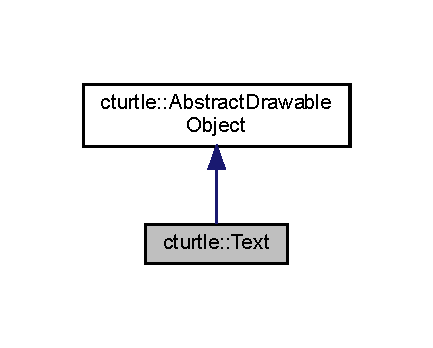
\includegraphics[width=208pt]{classcturtle_1_1Text__inherit__graph}
\end{center}
\end{figure}


Collaboration diagram for cturtle\+:\+:Text\+:
\nopagebreak
\begin{figure}[H]
\begin{center}
\leavevmode
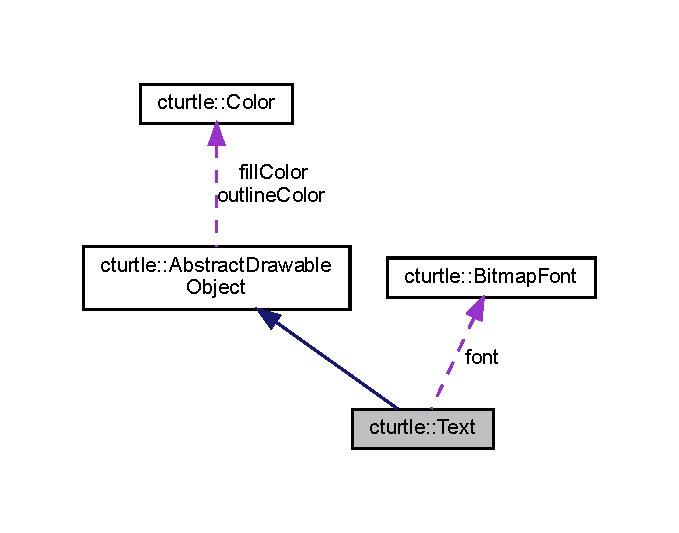
\includegraphics[width=208pt]{classcturtle_1_1Text__coll__graph}
\end{center}
\end{figure}
\subsection*{Public Member Functions}
\begin{DoxyCompactItemize}
\item 
\hyperlink{classcturtle_1_1Text_aad06f49d01be75cbfafedb64a38cfc29}{Text} ()
\item 
\mbox{\Hypertarget{classcturtle_1_1Text_a9adab9abc546c76b39feb594e0f4de1a}\label{classcturtle_1_1Text_a9adab9abc546c76b39feb594e0f4de1a}} 
{\bfseries Text} (const std\+::string \&\hyperlink{classcturtle_1_1Text_ac631d8199ccd9ae56f661e22acc157d9}{text}, \hyperlink{classcturtle_1_1Color}{Color} color)
\item 
\mbox{\Hypertarget{classcturtle_1_1Text_acea0ae681ef02899079547d852810687}\label{classcturtle_1_1Text_acea0ae681ef02899079547d852810687}} 
{\bfseries Text} (const \hyperlink{classcturtle_1_1Text}{Text} \&\hyperlink{classcturtle_1_1Text_acb0908ae70d1194d6e47a8f8ba51461a}{copy})
\item 
\mbox{\Hypertarget{classcturtle_1_1Text_acb0908ae70d1194d6e47a8f8ba51461a}\label{classcturtle_1_1Text_acb0908ae70d1194d6e47a8f8ba51461a}} 
\hyperlink{classcturtle_1_1AbstractDrawableObject}{Abstract\+Drawable\+Object} $\ast$ \hyperlink{classcturtle_1_1Text_acb0908ae70d1194d6e47a8f8ba51461a}{copy} () const
\begin{DoxyCompactList}\small\item\em Returns a pointer to a copy of this drawable object, allocated with N\+EW. Result Must be deleted at the responsibility of the invoker. \end{DoxyCompactList}\item 
void \hyperlink{classcturtle_1_1Text_a80003e4c447def1c7de8daf29a8fc5ec}{draw} (const \hyperlink{classcturtle_1_1Transform}{Transform} \&t, Image \&img\+Ref) const
\begin{DoxyCompactList}\small\item\em This function is intended to draw all applicable geometry in this object to the specified image, with the specified transform, with the specified color. This function is intended to be overloaded by child classes to draw applicable geometry to an image, acting as a canvas. \end{DoxyCompactList}\end{DoxyCompactItemize}
\subsection*{Public Attributes}
\begin{DoxyCompactItemize}
\item 
std\+::string \hyperlink{classcturtle_1_1Text_ac631d8199ccd9ae56f661e22acc157d9}{text}
\end{DoxyCompactItemize}


\subsection{Constructor \& Destructor Documentation}
\mbox{\Hypertarget{classcturtle_1_1Text_aad06f49d01be75cbfafedb64a38cfc29}\label{classcturtle_1_1Text_aad06f49d01be75cbfafedb64a38cfc29}} 
\index{cturtle\+::\+Text@{cturtle\+::\+Text}!Text@{Text}}
\index{Text@{Text}!cturtle\+::\+Text@{cturtle\+::\+Text}}
\subsubsection{\texorpdfstring{Text()}{Text()}}
{\footnotesize\ttfamily cturtle\+::\+Text\+::\+Text (\begin{DoxyParamCaption}{ }\end{DoxyParamCaption})\hspace{0.3cm}{\ttfamily [inline]}}

Blank default destructor. 

\subsection{Member Function Documentation}
\mbox{\Hypertarget{classcturtle_1_1Text_a80003e4c447def1c7de8daf29a8fc5ec}\label{classcturtle_1_1Text_a80003e4c447def1c7de8daf29a8fc5ec}} 
\index{cturtle\+::\+Text@{cturtle\+::\+Text}!draw@{draw}}
\index{draw@{draw}!cturtle\+::\+Text@{cturtle\+::\+Text}}
\subsubsection{\texorpdfstring{draw()}{draw()}}
{\footnotesize\ttfamily void cturtle\+::\+Text\+::draw (\begin{DoxyParamCaption}\item[{const \hyperlink{classcturtle_1_1Transform}{Transform} \&}]{t,  }\item[{Image \&}]{img\+Ref }\end{DoxyParamCaption}) const\hspace{0.3cm}{\ttfamily [inline]}, {\ttfamily [virtual]}}



This function is intended to draw all applicable geometry in this object to the specified image, with the specified transform, with the specified color. This function is intended to be overloaded by child classes to draw applicable geometry to an image, acting as a canvas. 


\begin{DoxyParams}{Parameters}
{\em t} & The transform at which to draw the geometry. \\
\hline
{\em img\+Ref} & The canvas on which to draw. \\
\hline
{\em c} & The color with to draw the geometry. \\
\hline
\end{DoxyParams}


Implements \hyperlink{classcturtle_1_1AbstractDrawableObject_a7b1ad1e9743d343e0fe577de3978bdad}{cturtle\+::\+Abstract\+Drawable\+Object}.



\subsection{Member Data Documentation}
\mbox{\Hypertarget{classcturtle_1_1Text_ac631d8199ccd9ae56f661e22acc157d9}\label{classcturtle_1_1Text_ac631d8199ccd9ae56f661e22acc157d9}} 
\index{cturtle\+::\+Text@{cturtle\+::\+Text}!text@{text}}
\index{text@{text}!cturtle\+::\+Text@{cturtle\+::\+Text}}
\subsubsection{\texorpdfstring{text}{text}}
{\footnotesize\ttfamily std\+::string cturtle\+::\+Text\+::text}

The text to draw. 

The documentation for this class was generated from the following file\+:\begin{DoxyCompactItemize}
\item 
C\+Turtle.\+hpp\end{DoxyCompactItemize}

\hypertarget{classcturtle_1_1Transform}{}\section{cturtle\+:\+:Transform Class Reference}
\label{classcturtle_1_1Transform}\index{cturtle\+::\+Transform@{cturtle\+::\+Transform}}


The \hyperlink{classcturtle_1_1Transform}{Transform} class provides a myriad of functions to simply transform points. This class it the backbone of almost all cartesian plane math in C\+Turtle. An adapted 3x3 matrix of the following link\+: \href{http://www.opengl-tutorial.org/beginners-tutorials/tutorial-3-matrices/}{\tt http\+://www.\+opengl-\/tutorial.\+org/beginners-\/tutorials/tutorial-\/3-\/matrices/}.  




{\ttfamily \#include $<$C\+Turtle.\+hpp$>$}

\subsection*{Public Member Functions}
\begin{DoxyCompactItemize}
\item 
\hyperlink{classcturtle_1_1Transform_a8b3953d07dfbe1f41ef5074144106d32}{Transform} ()
\item 
\hyperlink{classcturtle_1_1Transform_a007759937e9ad468e5ea41687571a417}{Transform} (const \hyperlink{classcturtle_1_1Transform}{Transform} \&other)
\begin{DoxyCompactList}\small\item\em Copy constructor. \end{DoxyCompactList}\item 
\hyperlink{classcturtle_1_1Transform}{Transform} \& \hyperlink{classcturtle_1_1Transform_a0102d86a459937597b4755650b94b4a2}{identity} ()
\begin{DoxyCompactList}\small\item\em Sets this transform to an identity. When you concatenate an identity transform onto another object, The resulting point is the same as it would have been pre-\/concatenation. Such is the point of an identity transform, and is why Affine\+Transforms are initialized to have this value. \end{DoxyCompactList}\item 
\mbox{\Hypertarget{classcturtle_1_1Transform_a77fe29e1fbf23aec97f988ca5f1bd3c3}\label{classcturtle_1_1Transform_a77fe29e1fbf23aec97f988ca5f1bd3c3}} 
bool \hyperlink{classcturtle_1_1Transform_a77fe29e1fbf23aec97f988ca5f1bd3c3}{operator==} (const \hyperlink{classcturtle_1_1Transform}{Transform} \&other) const
\begin{DoxyCompactList}\small\item\em Returns a boolean indicating if this transform is equivalent in value to the one specified. \end{DoxyCompactList}\item 
float \hyperlink{classcturtle_1_1Transform_ac7ab4863a65f6ee7d222be6bb01cc54c}{get\+ScaleX} () const
\begin{DoxyCompactList}\small\item\em Returns the X scale of this transform. \end{DoxyCompactList}\item 
float \hyperlink{classcturtle_1_1Transform_a7a47c8a4e32edfcccd871187dbd9680e}{get\+ScaleY} () const
\begin{DoxyCompactList}\small\item\em Returns the Y scale of this transform. \end{DoxyCompactList}\item 
float \hyperlink{classcturtle_1_1Transform_a341b1f4fe0055d1c27d3cbea61ef3788}{get\+TranslateX} () const
\begin{DoxyCompactList}\small\item\em Returns the X translation of this transform. \end{DoxyCompactList}\item 
float \hyperlink{classcturtle_1_1Transform_a9da2a0e256fdddbc0b5202c8d53a74bf}{get\+TranslateY} () const
\begin{DoxyCompactList}\small\item\em Returns the Y translation of this transform. \end{DoxyCompactList}\item 
float \hyperlink{classcturtle_1_1Transform_a1c879c9c239ca3a6af2d85c73b7e39b8}{get\+Rotation} () const
\begin{DoxyCompactList}\small\item\em Returns rotation of this transform, in radians. \end{DoxyCompactList}\item 
\hyperlink{classcturtle_1_1Transform}{Transform} \& \hyperlink{classcturtle_1_1Transform_ae0a81b79c7e737eadd880c20624acae3}{forward} (float distance)
\item 
\mbox{\Hypertarget{classcturtle_1_1Transform_ae52b78a68ee2005d0479b0347414ca28}\label{classcturtle_1_1Transform_ae52b78a68ee2005d0479b0347414ca28}} 
\hyperlink{classcturtle_1_1Transform}{Transform} \& {\bfseries backward} (float distance)
\item 
\hyperlink{classcturtle_1_1Transform}{Transform} \& \hyperlink{classcturtle_1_1Transform_a99366b0667eab2ea5f4f194f8500f94a}{set\+Translation} (int x, int y)
\begin{DoxyCompactList}\small\item\em Sets the translation of this transform. \end{DoxyCompactList}\item 
\hyperlink{structcturtle_1_1ivec2}{Point} \hyperlink{classcturtle_1_1Transform_a1458bf240e11c44e32c9acc483406aec}{get\+Translation} () const
\begin{DoxyCompactList}\small\item\em Returns the translation of this transform as a point. \end{DoxyCompactList}\item 
\hyperlink{classcturtle_1_1Transform}{Transform} \& \hyperlink{classcturtle_1_1Transform_a1ce9955dd58f54a64e3c9277c82456d1}{set\+TranslationX} (int x)
\begin{DoxyCompactList}\small\item\em Sets the X axis translation of this transform. \end{DoxyCompactList}\item 
\hyperlink{classcturtle_1_1Transform}{Transform} \& \hyperlink{classcturtle_1_1Transform_a6e861207764b8ca62152b99eb86a1f1a}{set\+TranslationY} (int y)
\begin{DoxyCompactList}\small\item\em Set the Y axis translation of this transform. \end{DoxyCompactList}\item 
\hyperlink{classcturtle_1_1Transform}{Transform} \& \hyperlink{classcturtle_1_1Transform_ae5029e23d426ff809a48ab56316dd989}{translate} (int x, int y)
\begin{DoxyCompactList}\small\item\em Translates this transform. \end{DoxyCompactList}\item 
\hyperlink{classcturtle_1_1Transform}{Transform} \& \hyperlink{classcturtle_1_1Transform_a0f94d37257362afb874f5df8a127613a}{rotate} (float theta)
\begin{DoxyCompactList}\small\item\em Rotates this transform. \end{DoxyCompactList}\item 
\hyperlink{classcturtle_1_1Transform}{Transform} \& \hyperlink{classcturtle_1_1Transform_aafed415c37989dcc34ed5cadd7366487}{set\+Rotation} (float val)
\begin{DoxyCompactList}\small\item\em Sets the rotation of this transform. \end{DoxyCompactList}\item 
\hyperlink{classcturtle_1_1Transform}{Transform} \& \hyperlink{classcturtle_1_1Transform_a985c6b26564267172e0f3d8ced7868e0}{rotate\+Around} (int x, int y, float theta)
\begin{DoxyCompactList}\small\item\em Rotates this transform around a specified point. \end{DoxyCompactList}\item 
\hyperlink{classcturtle_1_1Transform}{Transform} \& \hyperlink{classcturtle_1_1Transform_a460e371e701eed2d19c14c6e93725c82}{scale} (float sx, float sy)
\begin{DoxyCompactList}\small\item\em Applies a scale transformation to this transform. \end{DoxyCompactList}\item 
\hyperlink{classcturtle_1_1Transform}{Transform} \& \hyperlink{classcturtle_1_1Transform_add9d96d9ea677c39e2c6133e7f133aff}{concatenate} (const \hyperlink{classcturtle_1_1Transform}{Transform} \&t)
\begin{DoxyCompactList}\small\item\em Concatenates this \hyperlink{classcturtle_1_1Transform}{Transform} with another. \end{DoxyCompactList}\item 
\hyperlink{classcturtle_1_1Transform}{Transform} \hyperlink{classcturtle_1_1Transform_a52442d40b46368002c318f2167ff3db4}{copy\+Concatenate} (const \hyperlink{classcturtle_1_1Transform}{Transform} \&t) const
\begin{DoxyCompactList}\small\item\em Creates a copy of this transform, concatenates the input, and returns it. \end{DoxyCompactList}\item 
\hyperlink{classcturtle_1_1Transform}{Transform} \hyperlink{classcturtle_1_1Transform_aafca536c5297631923db197c225e8bf5}{lerp} (const \hyperlink{classcturtle_1_1Transform}{Transform} \&t, float progress) const
\begin{DoxyCompactList}\small\item\em Interpolates between this and the specified transform. Progress is a float in range of 0 to 1. \end{DoxyCompactList}\item 
void \hyperlink{classcturtle_1_1Transform_a5eb270c2614cc18c23623b24feb6968e}{assign} (const \hyperlink{classcturtle_1_1Transform}{Transform} \&t)
\begin{DoxyCompactList}\small\item\em Assigns the value of this transform to that of another. \end{DoxyCompactList}\item 
\hyperlink{structcturtle_1_1ivec2}{Point} \hyperlink{classcturtle_1_1Transform_aa8631732daaddc8336ed29f5462d1fef}{transform} (\hyperlink{structcturtle_1_1ivec2}{Point} in, \hyperlink{structcturtle_1_1ivec2}{Point} $\ast$dst=nullptr) const
\begin{DoxyCompactList}\small\item\em Transforms a point according to this transform. \end{DoxyCompactList}\item 
{\footnotesize template$<$typename I\+T\+E\+R\+\_\+T $>$ }\\void \hyperlink{classcturtle_1_1Transform_aae183c07fb323d0dfe8b3d633d59415c}{transform\+Set} (I\+T\+E\+R\+\_\+T cur, I\+T\+E\+R\+\_\+T end) const
\begin{DoxyCompactList}\small\item\em Transforms a set of points given a begin and end iterator. \end{DoxyCompactList}\item 
\hyperlink{structcturtle_1_1ivec2}{Point} \hyperlink{classcturtle_1_1Transform_afc24321e5d8da21c310fd830aa76da84}{operator()} (\hyperlink{structcturtle_1_1ivec2}{Point} in) const
\begin{DoxyCompactList}\small\item\em Operator overload to transform a single point. \end{DoxyCompactList}\end{DoxyCompactItemize}
\subsection*{Protected Types}
\begin{DoxyCompactItemize}
\item 
typedef std\+::array$<$ float, 9 $>$ \hyperlink{classcturtle_1_1Transform_a2952f427614626cb6b72553fb8451d8a}{mat\+\_\+t}
\end{DoxyCompactItemize}
\subsection*{Protected Member Functions}
\begin{DoxyCompactItemize}
\item 
float \& \hyperlink{classcturtle_1_1Transform_a640a1e38d034eb0b3878c4c56f014dd2}{at} (int row, int col)
\begin{DoxyCompactList}\small\item\em Returns a reference to the float the specified coordinate. \end{DoxyCompactList}\item 
float \hyperlink{classcturtle_1_1Transform_af6ab44503dfb32a56bbce3c8b2b5ea97}{at} (int row, int col) const
\begin{DoxyCompactList}\small\item\em Returns a copy of the float at the specified coordinate. \end{DoxyCompactList}\end{DoxyCompactItemize}
\subsection*{Protected Attributes}
\begin{DoxyCompactItemize}
\item 
\hyperlink{classcturtle_1_1Transform_a2952f427614626cb6b72553fb8451d8a}{mat\+\_\+t} \hyperlink{classcturtle_1_1Transform_a747be70a22109ecf9470c7ad75565c0c}{value}
\item 
float \hyperlink{classcturtle_1_1Transform_a79f7e11fb2b3d1093458100783cdd984}{rotation} = 0
\end{DoxyCompactItemize}


\subsection{Detailed Description}
The \hyperlink{classcturtle_1_1Transform}{Transform} class provides a myriad of functions to simply transform points. This class it the backbone of almost all cartesian plane math in C\+Turtle. An adapted 3x3 matrix of the following link\+: \href{http://www.opengl-tutorial.org/beginners-tutorials/tutorial-3-matrices/}{\tt http\+://www.\+opengl-\/tutorial.\+org/beginners-\/tutorials/tutorial-\/3-\/matrices/}. 

\subsection{Member Typedef Documentation}
\mbox{\Hypertarget{classcturtle_1_1Transform_a2952f427614626cb6b72553fb8451d8a}\label{classcturtle_1_1Transform_a2952f427614626cb6b72553fb8451d8a}} 
\index{cturtle\+::\+Transform@{cturtle\+::\+Transform}!mat\+\_\+t@{mat\+\_\+t}}
\index{mat\+\_\+t@{mat\+\_\+t}!cturtle\+::\+Transform@{cturtle\+::\+Transform}}
\subsubsection{\texorpdfstring{mat\+\_\+t}{mat\_t}}
{\footnotesize\ttfamily typedef std\+::array$<$float, 9$>$ \hyperlink{classcturtle_1_1Transform_a2952f427614626cb6b72553fb8451d8a}{cturtle\+::\+Transform\+::mat\+\_\+t}\hspace{0.3cm}{\ttfamily [protected]}}

The underlying matrix type. It\textquotesingle{}s defined simply as an array of 9 floats. Retrieved from coordinate pairs using (x$\ast$3+y) as indices. 

\subsection{Constructor \& Destructor Documentation}
\mbox{\Hypertarget{classcturtle_1_1Transform_a8b3953d07dfbe1f41ef5074144106d32}\label{classcturtle_1_1Transform_a8b3953d07dfbe1f41ef5074144106d32}} 
\index{cturtle\+::\+Transform@{cturtle\+::\+Transform}!Transform@{Transform}}
\index{Transform@{Transform}!cturtle\+::\+Transform@{cturtle\+::\+Transform}}
\subsubsection{\texorpdfstring{Transform()}{Transform()}\hspace{0.1cm}{\footnotesize\ttfamily [1/2]}}
{\footnotesize\ttfamily cturtle\+::\+Transform\+::\+Transform (\begin{DoxyParamCaption}{ }\end{DoxyParamCaption})\hspace{0.3cm}{\ttfamily [inline]}}

Constructs an empty transform. Initializes, by default, as an identity transform. \mbox{\Hypertarget{classcturtle_1_1Transform_a007759937e9ad468e5ea41687571a417}\label{classcturtle_1_1Transform_a007759937e9ad468e5ea41687571a417}} 
\index{cturtle\+::\+Transform@{cturtle\+::\+Transform}!Transform@{Transform}}
\index{Transform@{Transform}!cturtle\+::\+Transform@{cturtle\+::\+Transform}}
\subsubsection{\texorpdfstring{Transform()}{Transform()}\hspace{0.1cm}{\footnotesize\ttfamily [2/2]}}
{\footnotesize\ttfamily cturtle\+::\+Transform\+::\+Transform (\begin{DoxyParamCaption}\item[{const \hyperlink{classcturtle_1_1Transform}{Transform} \&}]{other }\end{DoxyParamCaption})\hspace{0.3cm}{\ttfamily [inline]}}



Copy constructor. 


\begin{DoxyParams}{Parameters}
{\em other} & The other transform from which to derive value. \\
\hline
\end{DoxyParams}


\subsection{Member Function Documentation}
\mbox{\Hypertarget{classcturtle_1_1Transform_a5eb270c2614cc18c23623b24feb6968e}\label{classcturtle_1_1Transform_a5eb270c2614cc18c23623b24feb6968e}} 
\index{cturtle\+::\+Transform@{cturtle\+::\+Transform}!assign@{assign}}
\index{assign@{assign}!cturtle\+::\+Transform@{cturtle\+::\+Transform}}
\subsubsection{\texorpdfstring{assign()}{assign()}}
{\footnotesize\ttfamily void cturtle\+::\+Transform\+::assign (\begin{DoxyParamCaption}\item[{const \hyperlink{classcturtle_1_1Transform}{Transform} \&}]{t }\end{DoxyParamCaption})\hspace{0.3cm}{\ttfamily [inline]}}



Assigns the value of this transform to that of another. 


\begin{DoxyParams}{Parameters}
{\em t} & The other transform to derive value from. \\
\hline
\end{DoxyParams}
\mbox{\Hypertarget{classcturtle_1_1Transform_a640a1e38d034eb0b3878c4c56f014dd2}\label{classcturtle_1_1Transform_a640a1e38d034eb0b3878c4c56f014dd2}} 
\index{cturtle\+::\+Transform@{cturtle\+::\+Transform}!at@{at}}
\index{at@{at}!cturtle\+::\+Transform@{cturtle\+::\+Transform}}
\subsubsection{\texorpdfstring{at()}{at()}\hspace{0.1cm}{\footnotesize\ttfamily [1/2]}}
{\footnotesize\ttfamily float\& cturtle\+::\+Transform\+::at (\begin{DoxyParamCaption}\item[{int}]{row,  }\item[{int}]{col }\end{DoxyParamCaption})\hspace{0.3cm}{\ttfamily [inline]}, {\ttfamily [protected]}}



Returns a reference to the float the specified coordinate. 


\begin{DoxyParams}{Parameters}
{\em row} & The specified row from which to get a component. \\
\hline
{\em col} & The specified column from which to get a component. \\
\hline
\end{DoxyParams}
\mbox{\Hypertarget{classcturtle_1_1Transform_af6ab44503dfb32a56bbce3c8b2b5ea97}\label{classcturtle_1_1Transform_af6ab44503dfb32a56bbce3c8b2b5ea97}} 
\index{cturtle\+::\+Transform@{cturtle\+::\+Transform}!at@{at}}
\index{at@{at}!cturtle\+::\+Transform@{cturtle\+::\+Transform}}
\subsubsection{\texorpdfstring{at()}{at()}\hspace{0.1cm}{\footnotesize\ttfamily [2/2]}}
{\footnotesize\ttfamily float cturtle\+::\+Transform\+::at (\begin{DoxyParamCaption}\item[{int}]{row,  }\item[{int}]{col }\end{DoxyParamCaption}) const\hspace{0.3cm}{\ttfamily [inline]}, {\ttfamily [protected]}}



Returns a copy of the float at the specified coordinate. 


\begin{DoxyParams}{Parameters}
{\em row} & The specified row from which to get a component. \\
\hline
{\em col} & The specified column from which to get a component. \\
\hline
\end{DoxyParams}
\mbox{\Hypertarget{classcturtle_1_1Transform_add9d96d9ea677c39e2c6133e7f133aff}\label{classcturtle_1_1Transform_add9d96d9ea677c39e2c6133e7f133aff}} 
\index{cturtle\+::\+Transform@{cturtle\+::\+Transform}!concatenate@{concatenate}}
\index{concatenate@{concatenate}!cturtle\+::\+Transform@{cturtle\+::\+Transform}}
\subsubsection{\texorpdfstring{concatenate()}{concatenate()}}
{\footnotesize\ttfamily \hyperlink{classcturtle_1_1Transform}{Transform}\& cturtle\+::\+Transform\+::concatenate (\begin{DoxyParamCaption}\item[{const \hyperlink{classcturtle_1_1Transform}{Transform} \&}]{t }\end{DoxyParamCaption})\hspace{0.3cm}{\ttfamily [inline]}}



Concatenates this \hyperlink{classcturtle_1_1Transform}{Transform} with another. 


\begin{DoxyParams}{Parameters}
{\em t} & The other \hyperlink{classcturtle_1_1Transform}{Transform} to concatenate with. \\
\hline
\end{DoxyParams}
\begin{DoxyReturn}{Returns}
A reference to this transform. (e.\+g, $\ast$this) 
\end{DoxyReturn}
\mbox{\Hypertarget{classcturtle_1_1Transform_a52442d40b46368002c318f2167ff3db4}\label{classcturtle_1_1Transform_a52442d40b46368002c318f2167ff3db4}} 
\index{cturtle\+::\+Transform@{cturtle\+::\+Transform}!copy\+Concatenate@{copy\+Concatenate}}
\index{copy\+Concatenate@{copy\+Concatenate}!cturtle\+::\+Transform@{cturtle\+::\+Transform}}
\subsubsection{\texorpdfstring{copy\+Concatenate()}{copyConcatenate()}}
{\footnotesize\ttfamily \hyperlink{classcturtle_1_1Transform}{Transform} cturtle\+::\+Transform\+::copy\+Concatenate (\begin{DoxyParamCaption}\item[{const \hyperlink{classcturtle_1_1Transform}{Transform} \&}]{t }\end{DoxyParamCaption}) const\hspace{0.3cm}{\ttfamily [inline]}}



Creates a copy of this transform, concatenates the input, and returns it. 


\begin{DoxyParams}{Parameters}
{\em t} & The input to concatenate onto the copy of this transform. \\
\hline
\end{DoxyParams}
\begin{DoxyReturn}{Returns}
Returns the concatenated copy of this transform. 
\end{DoxyReturn}
\mbox{\Hypertarget{classcturtle_1_1Transform_ae0a81b79c7e737eadd880c20624acae3}\label{classcturtle_1_1Transform_ae0a81b79c7e737eadd880c20624acae3}} 
\index{cturtle\+::\+Transform@{cturtle\+::\+Transform}!forward@{forward}}
\index{forward@{forward}!cturtle\+::\+Transform@{cturtle\+::\+Transform}}
\subsubsection{\texorpdfstring{forward()}{forward()}}
{\footnotesize\ttfamily \hyperlink{classcturtle_1_1Transform}{Transform}\& cturtle\+::\+Transform\+::forward (\begin{DoxyParamCaption}\item[{float}]{distance }\end{DoxyParamCaption})\hspace{0.3cm}{\ttfamily [inline]}}

Moves this transform \char`\"{}forward\char`\"{} according to its rotation. \mbox{\Hypertarget{classcturtle_1_1Transform_a1c879c9c239ca3a6af2d85c73b7e39b8}\label{classcturtle_1_1Transform_a1c879c9c239ca3a6af2d85c73b7e39b8}} 
\index{cturtle\+::\+Transform@{cturtle\+::\+Transform}!get\+Rotation@{get\+Rotation}}
\index{get\+Rotation@{get\+Rotation}!cturtle\+::\+Transform@{cturtle\+::\+Transform}}
\subsubsection{\texorpdfstring{get\+Rotation()}{getRotation()}}
{\footnotesize\ttfamily float cturtle\+::\+Transform\+::get\+Rotation (\begin{DoxyParamCaption}{ }\end{DoxyParamCaption}) const\hspace{0.3cm}{\ttfamily [inline]}}



Returns rotation of this transform, in radians. 

\begin{DoxyReturn}{Returns}
The rotation of this transform, in radians. 
\end{DoxyReturn}
\mbox{\Hypertarget{classcturtle_1_1Transform_ac7ab4863a65f6ee7d222be6bb01cc54c}\label{classcturtle_1_1Transform_ac7ab4863a65f6ee7d222be6bb01cc54c}} 
\index{cturtle\+::\+Transform@{cturtle\+::\+Transform}!get\+ScaleX@{get\+ScaleX}}
\index{get\+ScaleX@{get\+ScaleX}!cturtle\+::\+Transform@{cturtle\+::\+Transform}}
\subsubsection{\texorpdfstring{get\+Scale\+X()}{getScaleX()}}
{\footnotesize\ttfamily float cturtle\+::\+Transform\+::get\+ScaleX (\begin{DoxyParamCaption}{ }\end{DoxyParamCaption}) const\hspace{0.3cm}{\ttfamily [inline]}}



Returns the X scale of this transform. 

\begin{DoxyReturn}{Returns}
Returns the X scale of this transform. 
\end{DoxyReturn}
\mbox{\Hypertarget{classcturtle_1_1Transform_a7a47c8a4e32edfcccd871187dbd9680e}\label{classcturtle_1_1Transform_a7a47c8a4e32edfcccd871187dbd9680e}} 
\index{cturtle\+::\+Transform@{cturtle\+::\+Transform}!get\+ScaleY@{get\+ScaleY}}
\index{get\+ScaleY@{get\+ScaleY}!cturtle\+::\+Transform@{cturtle\+::\+Transform}}
\subsubsection{\texorpdfstring{get\+Scale\+Y()}{getScaleY()}}
{\footnotesize\ttfamily float cturtle\+::\+Transform\+::get\+ScaleY (\begin{DoxyParamCaption}{ }\end{DoxyParamCaption}) const\hspace{0.3cm}{\ttfamily [inline]}}



Returns the Y scale of this transform. 

\begin{DoxyReturn}{Returns}
Returns the Y scale of this transform. 
\end{DoxyReturn}
\mbox{\Hypertarget{classcturtle_1_1Transform_a341b1f4fe0055d1c27d3cbea61ef3788}\label{classcturtle_1_1Transform_a341b1f4fe0055d1c27d3cbea61ef3788}} 
\index{cturtle\+::\+Transform@{cturtle\+::\+Transform}!get\+TranslateX@{get\+TranslateX}}
\index{get\+TranslateX@{get\+TranslateX}!cturtle\+::\+Transform@{cturtle\+::\+Transform}}
\subsubsection{\texorpdfstring{get\+Translate\+X()}{getTranslateX()}}
{\footnotesize\ttfamily float cturtle\+::\+Transform\+::get\+TranslateX (\begin{DoxyParamCaption}{ }\end{DoxyParamCaption}) const\hspace{0.3cm}{\ttfamily [inline]}}



Returns the X translation of this transform. 

\begin{DoxyReturn}{Returns}
Returns the X translation of this transform. 
\end{DoxyReturn}
\mbox{\Hypertarget{classcturtle_1_1Transform_a9da2a0e256fdddbc0b5202c8d53a74bf}\label{classcturtle_1_1Transform_a9da2a0e256fdddbc0b5202c8d53a74bf}} 
\index{cturtle\+::\+Transform@{cturtle\+::\+Transform}!get\+TranslateY@{get\+TranslateY}}
\index{get\+TranslateY@{get\+TranslateY}!cturtle\+::\+Transform@{cturtle\+::\+Transform}}
\subsubsection{\texorpdfstring{get\+Translate\+Y()}{getTranslateY()}}
{\footnotesize\ttfamily float cturtle\+::\+Transform\+::get\+TranslateY (\begin{DoxyParamCaption}{ }\end{DoxyParamCaption}) const\hspace{0.3cm}{\ttfamily [inline]}}



Returns the Y translation of this transform. 

\begin{DoxyReturn}{Returns}
Returns the Y translation of this transform. 
\end{DoxyReturn}
\mbox{\Hypertarget{classcturtle_1_1Transform_a1458bf240e11c44e32c9acc483406aec}\label{classcturtle_1_1Transform_a1458bf240e11c44e32c9acc483406aec}} 
\index{cturtle\+::\+Transform@{cturtle\+::\+Transform}!get\+Translation@{get\+Translation}}
\index{get\+Translation@{get\+Translation}!cturtle\+::\+Transform@{cturtle\+::\+Transform}}
\subsubsection{\texorpdfstring{get\+Translation()}{getTranslation()}}
{\footnotesize\ttfamily \hyperlink{structcturtle_1_1ivec2}{Point} cturtle\+::\+Transform\+::get\+Translation (\begin{DoxyParamCaption}{ }\end{DoxyParamCaption}) const\hspace{0.3cm}{\ttfamily [inline]}}



Returns the translation of this transform as a point. 

\begin{DoxyReturn}{Returns}
The point which represents the transform. 
\end{DoxyReturn}
\mbox{\Hypertarget{classcturtle_1_1Transform_a0102d86a459937597b4755650b94b4a2}\label{classcturtle_1_1Transform_a0102d86a459937597b4755650b94b4a2}} 
\index{cturtle\+::\+Transform@{cturtle\+::\+Transform}!identity@{identity}}
\index{identity@{identity}!cturtle\+::\+Transform@{cturtle\+::\+Transform}}
\subsubsection{\texorpdfstring{identity()}{identity()}}
{\footnotesize\ttfamily \hyperlink{classcturtle_1_1Transform}{Transform}\& cturtle\+::\+Transform\+::identity (\begin{DoxyParamCaption}{ }\end{DoxyParamCaption})\hspace{0.3cm}{\ttfamily [inline]}}



Sets this transform to an identity. When you concatenate an identity transform onto another object, The resulting point is the same as it would have been pre-\/concatenation. Such is the point of an identity transform, and is why Affine\+Transforms are initialized to have this value. 

\begin{DoxyReturn}{Returns}
A reference to this transform. (e.\+g, $\ast$this) 
\end{DoxyReturn}
\mbox{\Hypertarget{classcturtle_1_1Transform_aafca536c5297631923db197c225e8bf5}\label{classcturtle_1_1Transform_aafca536c5297631923db197c225e8bf5}} 
\index{cturtle\+::\+Transform@{cturtle\+::\+Transform}!lerp@{lerp}}
\index{lerp@{lerp}!cturtle\+::\+Transform@{cturtle\+::\+Transform}}
\subsubsection{\texorpdfstring{lerp()}{lerp()}}
{\footnotesize\ttfamily \hyperlink{classcturtle_1_1Transform}{Transform} cturtle\+::\+Transform\+::lerp (\begin{DoxyParamCaption}\item[{const \hyperlink{classcturtle_1_1Transform}{Transform} \&}]{t,  }\item[{float}]{progress }\end{DoxyParamCaption}) const\hspace{0.3cm}{\ttfamily [inline]}}



Interpolates between this and the specified transform. Progress is a float in range of 0 to 1. 


\begin{DoxyParams}{Parameters}
{\em t} & The destination transform. \\
\hline
{\em progress} & A progress float in range of 0 to 1. \\
\hline
\end{DoxyParams}
\begin{DoxyReturn}{Returns}
The resulting interpolated transform. 
\end{DoxyReturn}
\mbox{\Hypertarget{classcturtle_1_1Transform_afc24321e5d8da21c310fd830aa76da84}\label{classcturtle_1_1Transform_afc24321e5d8da21c310fd830aa76da84}} 
\index{cturtle\+::\+Transform@{cturtle\+::\+Transform}!operator()@{operator()}}
\index{operator()@{operator()}!cturtle\+::\+Transform@{cturtle\+::\+Transform}}
\subsubsection{\texorpdfstring{operator()()}{operator()()}}
{\footnotesize\ttfamily \hyperlink{structcturtle_1_1ivec2}{Point} cturtle\+::\+Transform\+::operator() (\begin{DoxyParamCaption}\item[{\hyperlink{structcturtle_1_1ivec2}{Point}}]{in }\end{DoxyParamCaption}) const\hspace{0.3cm}{\ttfamily [inline]}}



Operator overload to transform a single point. 


\begin{DoxyParams}{Parameters}
{\em in} & The point to transform. \\
\hline
\end{DoxyParams}
\mbox{\Hypertarget{classcturtle_1_1Transform_a0f94d37257362afb874f5df8a127613a}\label{classcturtle_1_1Transform_a0f94d37257362afb874f5df8a127613a}} 
\index{cturtle\+::\+Transform@{cturtle\+::\+Transform}!rotate@{rotate}}
\index{rotate@{rotate}!cturtle\+::\+Transform@{cturtle\+::\+Transform}}
\subsubsection{\texorpdfstring{rotate()}{rotate()}}
{\footnotesize\ttfamily \hyperlink{classcturtle_1_1Transform}{Transform}\& cturtle\+::\+Transform\+::rotate (\begin{DoxyParamCaption}\item[{float}]{theta }\end{DoxyParamCaption})\hspace{0.3cm}{\ttfamily [inline]}}



Rotates this transform. 


\begin{DoxyParams}{Parameters}
{\em theta} & The angle at which to rotate, in radians \\
\hline
\end{DoxyParams}
\begin{DoxyReturn}{Returns}
A reference to this transform. (e.\+g, $\ast$this) 
\end{DoxyReturn}
\mbox{\Hypertarget{classcturtle_1_1Transform_a985c6b26564267172e0f3d8ced7868e0}\label{classcturtle_1_1Transform_a985c6b26564267172e0f3d8ced7868e0}} 
\index{cturtle\+::\+Transform@{cturtle\+::\+Transform}!rotate\+Around@{rotate\+Around}}
\index{rotate\+Around@{rotate\+Around}!cturtle\+::\+Transform@{cturtle\+::\+Transform}}
\subsubsection{\texorpdfstring{rotate\+Around()}{rotateAround()}}
{\footnotesize\ttfamily \hyperlink{classcturtle_1_1Transform}{Transform}\& cturtle\+::\+Transform\+::rotate\+Around (\begin{DoxyParamCaption}\item[{int}]{x,  }\item[{int}]{y,  }\item[{float}]{theta }\end{DoxyParamCaption})\hspace{0.3cm}{\ttfamily [inline]}}



Rotates this transform around a specified point. 


\begin{DoxyParams}{Parameters}
{\em x} & The X coordinate to rotate around. \\
\hline
{\em y} & The Y coordinate to rotate around. \\
\hline
{\em theta} & The angle at which to rotate, in radians \\
\hline
\end{DoxyParams}
\begin{DoxyReturn}{Returns}
A reference to this transform. (e.\+g, $\ast$this) 
\end{DoxyReturn}
\mbox{\Hypertarget{classcturtle_1_1Transform_a460e371e701eed2d19c14c6e93725c82}\label{classcturtle_1_1Transform_a460e371e701eed2d19c14c6e93725c82}} 
\index{cturtle\+::\+Transform@{cturtle\+::\+Transform}!scale@{scale}}
\index{scale@{scale}!cturtle\+::\+Transform@{cturtle\+::\+Transform}}
\subsubsection{\texorpdfstring{scale()}{scale()}}
{\footnotesize\ttfamily \hyperlink{classcturtle_1_1Transform}{Transform}\& cturtle\+::\+Transform\+::scale (\begin{DoxyParamCaption}\item[{float}]{sx,  }\item[{float}]{sy }\end{DoxyParamCaption})\hspace{0.3cm}{\ttfamily [inline]}}



Applies a scale transformation to this transform. 


\begin{DoxyParams}{Parameters}
{\em sx} & The X axis scale factor. \\
\hline
{\em sy} & The Y axis scale factor. \\
\hline
\end{DoxyParams}
\mbox{\Hypertarget{classcturtle_1_1Transform_aafed415c37989dcc34ed5cadd7366487}\label{classcturtle_1_1Transform_aafed415c37989dcc34ed5cadd7366487}} 
\index{cturtle\+::\+Transform@{cturtle\+::\+Transform}!set\+Rotation@{set\+Rotation}}
\index{set\+Rotation@{set\+Rotation}!cturtle\+::\+Transform@{cturtle\+::\+Transform}}
\subsubsection{\texorpdfstring{set\+Rotation()}{setRotation()}}
{\footnotesize\ttfamily \hyperlink{classcturtle_1_1Transform}{Transform}\& cturtle\+::\+Transform\+::set\+Rotation (\begin{DoxyParamCaption}\item[{float}]{val }\end{DoxyParamCaption})\hspace{0.3cm}{\ttfamily [inline]}}



Sets the rotation of this transform. 


\begin{DoxyParams}{Parameters}
{\em val} & The angle at which to rotate, in radians. \\
\hline
\end{DoxyParams}
\begin{DoxyReturn}{Returns}
A reference to this transform. (e.\+g, $\ast$this) 
\end{DoxyReturn}
\mbox{\Hypertarget{classcturtle_1_1Transform_a99366b0667eab2ea5f4f194f8500f94a}\label{classcturtle_1_1Transform_a99366b0667eab2ea5f4f194f8500f94a}} 
\index{cturtle\+::\+Transform@{cturtle\+::\+Transform}!set\+Translation@{set\+Translation}}
\index{set\+Translation@{set\+Translation}!cturtle\+::\+Transform@{cturtle\+::\+Transform}}
\subsubsection{\texorpdfstring{set\+Translation()}{setTranslation()}}
{\footnotesize\ttfamily \hyperlink{classcturtle_1_1Transform}{Transform}\& cturtle\+::\+Transform\+::set\+Translation (\begin{DoxyParamCaption}\item[{int}]{x,  }\item[{int}]{y }\end{DoxyParamCaption})\hspace{0.3cm}{\ttfamily [inline]}}



Sets the translation of this transform. 


\begin{DoxyParams}{Parameters}
{\em x} & The number of units, or pixels, to transform on the X axis. \\
\hline
{\em y} & The number of units, or pixels, to transform on the Y axis. \\
\hline
\end{DoxyParams}
\begin{DoxyReturn}{Returns}
A reference to this transform. (e.\+g, $\ast$this) 
\end{DoxyReturn}
\mbox{\Hypertarget{classcturtle_1_1Transform_a1ce9955dd58f54a64e3c9277c82456d1}\label{classcturtle_1_1Transform_a1ce9955dd58f54a64e3c9277c82456d1}} 
\index{cturtle\+::\+Transform@{cturtle\+::\+Transform}!set\+TranslationX@{set\+TranslationX}}
\index{set\+TranslationX@{set\+TranslationX}!cturtle\+::\+Transform@{cturtle\+::\+Transform}}
\subsubsection{\texorpdfstring{set\+Translation\+X()}{setTranslationX()}}
{\footnotesize\ttfamily \hyperlink{classcturtle_1_1Transform}{Transform}\& cturtle\+::\+Transform\+::set\+TranslationX (\begin{DoxyParamCaption}\item[{int}]{x }\end{DoxyParamCaption})\hspace{0.3cm}{\ttfamily [inline]}}



Sets the X axis translation of this transform. 


\begin{DoxyParams}{Parameters}
{\em x} & The number of units, or pixels, to transform on the X axis. \\
\hline
\end{DoxyParams}
\begin{DoxyReturn}{Returns}
A reference to this transform. (e.\+g, $\ast$this) 
\end{DoxyReturn}
\mbox{\Hypertarget{classcturtle_1_1Transform_a6e861207764b8ca62152b99eb86a1f1a}\label{classcturtle_1_1Transform_a6e861207764b8ca62152b99eb86a1f1a}} 
\index{cturtle\+::\+Transform@{cturtle\+::\+Transform}!set\+TranslationY@{set\+TranslationY}}
\index{set\+TranslationY@{set\+TranslationY}!cturtle\+::\+Transform@{cturtle\+::\+Transform}}
\subsubsection{\texorpdfstring{set\+Translation\+Y()}{setTranslationY()}}
{\footnotesize\ttfamily \hyperlink{classcturtle_1_1Transform}{Transform}\& cturtle\+::\+Transform\+::set\+TranslationY (\begin{DoxyParamCaption}\item[{int}]{y }\end{DoxyParamCaption})\hspace{0.3cm}{\ttfamily [inline]}}



Set the Y axis translation of this transform. 


\begin{DoxyParams}{Parameters}
{\em y} & The number of units, or pixels, to transform on the Y axis. \\
\hline
\end{DoxyParams}
\begin{DoxyReturn}{Returns}
A reference to this transform. (e.\+g, $\ast$this) 
\end{DoxyReturn}
\mbox{\Hypertarget{classcturtle_1_1Transform_aa8631732daaddc8336ed29f5462d1fef}\label{classcturtle_1_1Transform_aa8631732daaddc8336ed29f5462d1fef}} 
\index{cturtle\+::\+Transform@{cturtle\+::\+Transform}!transform@{transform}}
\index{transform@{transform}!cturtle\+::\+Transform@{cturtle\+::\+Transform}}
\subsubsection{\texorpdfstring{transform()}{transform()}}
{\footnotesize\ttfamily \hyperlink{structcturtle_1_1ivec2}{Point} cturtle\+::\+Transform\+::transform (\begin{DoxyParamCaption}\item[{\hyperlink{structcturtle_1_1ivec2}{Point}}]{in,  }\item[{\hyperlink{structcturtle_1_1ivec2}{Point} $\ast$}]{dst = {\ttfamily nullptr} }\end{DoxyParamCaption}) const\hspace{0.3cm}{\ttfamily [inline]}}



Transforms a point according to this transform. 


\begin{DoxyParams}{Parameters}
{\em in} & The input point. \\
\hline
{\em dst} & The destination pointer to store the value. Can be same as input.. \\
\hline
\end{DoxyParams}
\begin{DoxyReturn}{Returns}
Returns the translated point. 

Also assigns the value of dst pointer to the result. 
\end{DoxyReturn}
\mbox{\Hypertarget{classcturtle_1_1Transform_aae183c07fb323d0dfe8b3d633d59415c}\label{classcturtle_1_1Transform_aae183c07fb323d0dfe8b3d633d59415c}} 
\index{cturtle\+::\+Transform@{cturtle\+::\+Transform}!transform\+Set@{transform\+Set}}
\index{transform\+Set@{transform\+Set}!cturtle\+::\+Transform@{cturtle\+::\+Transform}}
\subsubsection{\texorpdfstring{transform\+Set()}{transformSet()}}
{\footnotesize\ttfamily template$<$typename I\+T\+E\+R\+\_\+T $>$ \\
void cturtle\+::\+Transform\+::transform\+Set (\begin{DoxyParamCaption}\item[{I\+T\+E\+R\+\_\+T}]{cur,  }\item[{I\+T\+E\+R\+\_\+T}]{end }\end{DoxyParamCaption}) const\hspace{0.3cm}{\ttfamily [inline]}}



Transforms a set of points given a begin and end iterator. 


\begin{DoxyParams}{Parameters}
{\em cur} & The beginning iterator of a set. \\
\hline
{\em end} & The ending iterator of a set. \\
\hline
\end{DoxyParams}
\mbox{\Hypertarget{classcturtle_1_1Transform_ae5029e23d426ff809a48ab56316dd989}\label{classcturtle_1_1Transform_ae5029e23d426ff809a48ab56316dd989}} 
\index{cturtle\+::\+Transform@{cturtle\+::\+Transform}!translate@{translate}}
\index{translate@{translate}!cturtle\+::\+Transform@{cturtle\+::\+Transform}}
\subsubsection{\texorpdfstring{translate()}{translate()}}
{\footnotesize\ttfamily \hyperlink{classcturtle_1_1Transform}{Transform}\& cturtle\+::\+Transform\+::translate (\begin{DoxyParamCaption}\item[{int}]{x,  }\item[{int}]{y }\end{DoxyParamCaption})\hspace{0.3cm}{\ttfamily [inline]}}



Translates this transform. 


\begin{DoxyParams}{Parameters}
{\em x} & The number of units, or pixels, to transform on the X axis. \\
\hline
{\em y} & The number of units, or pixels, to transform on the Y axis. \\
\hline
\end{DoxyParams}
\begin{DoxyReturn}{Returns}
A reference to this transform. (e.\+g, $\ast$this) 
\end{DoxyReturn}


\subsection{Member Data Documentation}
\mbox{\Hypertarget{classcturtle_1_1Transform_a79f7e11fb2b3d1093458100783cdd984}\label{classcturtle_1_1Transform_a79f7e11fb2b3d1093458100783cdd984}} 
\index{cturtle\+::\+Transform@{cturtle\+::\+Transform}!rotation@{rotation}}
\index{rotation@{rotation}!cturtle\+::\+Transform@{cturtle\+::\+Transform}}
\subsubsection{\texorpdfstring{rotation}{rotation}}
{\footnotesize\ttfamily float cturtle\+::\+Transform\+::rotation = 0\hspace{0.3cm}{\ttfamily [protected]}}

The rotation of this transform, in radians. \mbox{\Hypertarget{classcturtle_1_1Transform_a747be70a22109ecf9470c7ad75565c0c}\label{classcturtle_1_1Transform_a747be70a22109ecf9470c7ad75565c0c}} 
\index{cturtle\+::\+Transform@{cturtle\+::\+Transform}!value@{value}}
\index{value@{value}!cturtle\+::\+Transform@{cturtle\+::\+Transform}}
\subsubsection{\texorpdfstring{value}{value}}
{\footnotesize\ttfamily \hyperlink{classcturtle_1_1Transform_a2952f427614626cb6b72553fb8451d8a}{mat\+\_\+t} cturtle\+::\+Transform\+::value\hspace{0.3cm}{\ttfamily [protected]}}

The value of this transform. 

The documentation for this class was generated from the following file\+:\begin{DoxyCompactItemize}
\item 
C\+Turtle.\+hpp\end{DoxyCompactItemize}

\hypertarget{classcturtle_1_1Turtle}{}\section{cturtle\+:\+:Turtle Class Reference}
\label{classcturtle_1_1Turtle}\index{cturtle\+::\+Turtle@{cturtle\+::\+Turtle}}


{\ttfamily \#include $<$C\+Turtle.\+hpp$>$}



Collaboration diagram for cturtle\+:\+:Turtle\+:
\nopagebreak
\begin{figure}[H]
\begin{center}
\leavevmode
\includegraphics[width=350pt]{classcturtle_1_1Turtle__coll__graph}
\end{center}
\end{figure}
\subsection*{Public Member Functions}
\begin{DoxyCompactItemize}
\item 
\mbox{\Hypertarget{classcturtle_1_1Turtle_af819a08c50a1eaceae945e69c4c7968a}\label{classcturtle_1_1Turtle_af819a08c50a1eaceae945e69c4c7968a}} 
{\bfseries Turtle} (\hyperlink{classcturtle_1_1AbstractTurtleScreen}{Abstract\+Turtle\+Screen} \&scr)
\item 
\mbox{\Hypertarget{classcturtle_1_1Turtle_a472d13726408a2c4f0820a9365d7822b}\label{classcturtle_1_1Turtle_a472d13726408a2c4f0820a9365d7822b}} 
void \hyperlink{classcturtle_1_1Turtle_a472d13726408a2c4f0820a9365d7822b}{forward} (int pixels)
\begin{DoxyCompactList}\small\item\em Moves the turtle forward the specified number of pixels. \end{DoxyCompactList}\item 
void \hyperlink{classcturtle_1_1Turtle_a2a9fa6b316c96af547eb90b44fbacdc0}{fd} (int pixels)
\begin{DoxyCompactList}\small\item\em Moves the turtle forward the specified number of pixels. \end{DoxyCompactList}\item 
\mbox{\Hypertarget{classcturtle_1_1Turtle_a2fd24ae80f39ed0598e1d3b2458b6b7b}\label{classcturtle_1_1Turtle_a2fd24ae80f39ed0598e1d3b2458b6b7b}} 
void \hyperlink{classcturtle_1_1Turtle_a2fd24ae80f39ed0598e1d3b2458b6b7b}{backward} (int pixels)
\begin{DoxyCompactList}\small\item\em Moves the turtle backward the specified number of pixels. \end{DoxyCompactList}\item 
void \hyperlink{classcturtle_1_1Turtle_a3f1ce4b0c550d890f8bfc7e6a02ea1ef}{bk} (int pixels)
\begin{DoxyCompactList}\small\item\em Moves the turtle backward the specified number of pixels. \end{DoxyCompactList}\item 
void \hyperlink{classcturtle_1_1Turtle_a3df431a36f6b1efa56c6b885ae22fde9}{back} (int pixels)
\begin{DoxyCompactList}\small\item\em Moves the turtle backward the specified number of pixels. \end{DoxyCompactList}\item 
void \hyperlink{classcturtle_1_1Turtle_a3586f116fccc417ffa74c115ec3eef54}{right} (float amt)
\begin{DoxyCompactList}\small\item\em Rotates the turtle the specified number of units to the right. The unit by which the input is specified is determined by the current angle mode. The difference between Clockwise and Counterclockwise is determined by the current screen\textquotesingle{}s mode. \end{DoxyCompactList}\item 
void \hyperlink{classcturtle_1_1Turtle_a5416304d65c9bbebe0fabd9914123a79}{rt} (float angle)
\begin{DoxyCompactList}\small\item\em Rotates the turtle the specified number of units to the right. The unit by which the input is specified is determined by the current angle mode. The difference between Clockwise and Counterclockwise is determined by the current screen\textquotesingle{}s mode. \end{DoxyCompactList}\item 
void \hyperlink{classcturtle_1_1Turtle_a60b8d0d7f9a80e4bca57bf3a788a6c01}{left} (float amt)
\begin{DoxyCompactList}\small\item\em Rotates the turtle the specified number of units to the left. The unit by which the input is specified is determined by the current angle mode. The difference between Clockwise and Counterclockwise is determined by the current screen\textquotesingle{}s mode. \end{DoxyCompactList}\item 
void \hyperlink{classcturtle_1_1Turtle_a4858ca94ff49171c615d319a307acb8d}{lt} (float angle)
\begin{DoxyCompactList}\small\item\em Rotates the turtle the specified number of units to the left. The unit by which the input is specified is determined by the current angle mode. The difference between Clockwise and Counterclockwise is determined by the current screen\textquotesingle{}s mode. \end{DoxyCompactList}\item 
\mbox{\Hypertarget{classcturtle_1_1Turtle_a1ad8303d1ec02fb9d49b88946b73abf7}\label{classcturtle_1_1Turtle_a1ad8303d1ec02fb9d49b88946b73abf7}} 
void \hyperlink{classcturtle_1_1Turtle_a1ad8303d1ec02fb9d49b88946b73abf7}{go\+To} (int x, int y)
\begin{DoxyCompactList}\small\item\em Sets the transform location of this turtle. \end{DoxyCompactList}\item 
\mbox{\Hypertarget{classcturtle_1_1Turtle_aebaca8328fa32d5fb286ad99a57b62fc}\label{classcturtle_1_1Turtle_aebaca8328fa32d5fb286ad99a57b62fc}} 
void \hyperlink{classcturtle_1_1Turtle_aebaca8328fa32d5fb286ad99a57b62fc}{go\+To} (const \hyperlink{structcturtle_1_1ivec2}{Point} \&pt)
\begin{DoxyCompactList}\small\item\em Sets the transform location of this turtle. \end{DoxyCompactList}\item 
void \hyperlink{classcturtle_1_1Turtle_ab7e2193a04b72e94069fcccd85fa40db}{setpos} (int x, int y)
\begin{DoxyCompactList}\small\item\em Sets the transform location of this turtle. \end{DoxyCompactList}\item 
void \hyperlink{classcturtle_1_1Turtle_a72b2958266efc5b3aea86a459bd04d0b}{setpos} (const \hyperlink{structcturtle_1_1ivec2}{Point} \&pt)
\begin{DoxyCompactList}\small\item\em Sets the transform location of this turtle. \end{DoxyCompactList}\item 
void \hyperlink{classcturtle_1_1Turtle_a5e9dd0e59f48e49719dd4e3bd06a82f1}{setposition} (int x, int y)
\begin{DoxyCompactList}\small\item\em Sets the transform location of this turtle. \end{DoxyCompactList}\item 
void \hyperlink{classcturtle_1_1Turtle_a7a4726103a42d73006357cc12ce79b72}{setposition} (const \hyperlink{structcturtle_1_1ivec2}{Point} \&pt)
\begin{DoxyCompactList}\small\item\em Sets the transform location of this turtle. \end{DoxyCompactList}\item 
\mbox{\Hypertarget{classcturtle_1_1Turtle_a647d02a7847eef248c45b84251f6639c}\label{classcturtle_1_1Turtle_a647d02a7847eef248c45b84251f6639c}} 
void \hyperlink{classcturtle_1_1Turtle_a647d02a7847eef248c45b84251f6639c}{setx} (int x)
\begin{DoxyCompactList}\small\item\em Sets the X-\/axis transform location of this turtle. \end{DoxyCompactList}\item 
\mbox{\Hypertarget{classcturtle_1_1Turtle_aeee8075a33445d89a060c4faa17f9e5c}\label{classcturtle_1_1Turtle_aeee8075a33445d89a060c4faa17f9e5c}} 
void \hyperlink{classcturtle_1_1Turtle_aeee8075a33445d89a060c4faa17f9e5c}{sety} (int y)
\begin{DoxyCompactList}\small\item\em Sets the Y-\/axis transform location of this turtle. \end{DoxyCompactList}\item 
void \hyperlink{classcturtle_1_1Turtle_aea45fc1d0f00b82fc64a0f97dd6c1ea2}{shift} (int x, int y)
\item 
void \hyperlink{classcturtle_1_1Turtle_a4eb2630341ea5bb922c74f214037b361}{setheading} (float angle)
\begin{DoxyCompactList}\small\item\em Sets the rotation of this turtle. The unit by which the input is specified is determined by the current angle mode. The difference between Clockwise and Counterclockwise is determined by the current screen\textquotesingle{}s mode. \end{DoxyCompactList}\item 
int \hyperlink{classcturtle_1_1Turtle_a4a6824b53f70323402d4e972f6da360c}{distance} (int x, int y)
\item 
int \hyperlink{classcturtle_1_1Turtle_aa8b64c7361639dec2eafedaf640a0ebd}{distance} (const \hyperlink{structcturtle_1_1ivec2}{Point} \&pt)
\item 
void \hyperlink{classcturtle_1_1Turtle_a2f578819830001dfb6694813f9a4aa19}{seth} (float angle)
\begin{DoxyCompactList}\small\item\em Sets the rotation of this turtle. The unit by which the input is specified is determined by the current angle mode. The difference between Clockwise and Counterclockwise is determined by the current screen\textquotesingle{}s mode. \end{DoxyCompactList}\item 
float \hyperlink{classcturtle_1_1Turtle_a1ac8961a3d5d3044b3f3f011778b51bf}{towards} (int x, int y)
\begin{DoxyCompactList}\small\item\em Returns the angle between the line of the current turtle transform to the given point. \end{DoxyCompactList}\item 
float \hyperlink{classcturtle_1_1Turtle_ab625cf304b44417c7d3cacd65b372d37}{towards} (const \hyperlink{structcturtle_1_1ivec2}{Point} \&pt)
\begin{DoxyCompactList}\small\item\em Returns the angle between the line of the current turtle transform to the given point. \end{DoxyCompactList}\item 
float \hyperlink{classcturtle_1_1Turtle_a5c90aa6dea03e88f202dcadc4ff77354}{heading} ()
\item 
void \hyperlink{classcturtle_1_1Turtle_ab6558ff8b547bfb54a68c55259f7bb32}{home} ()
\item 
void \hyperlink{classcturtle_1_1Turtle_a6ce4e8065581887d006f420d0e93967e}{circle} (int radius, int steps, \hyperlink{classcturtle_1_1Color}{Color} color)
\begin{DoxyCompactList}\small\item\em Adds a circle to the screen. \end{DoxyCompactList}\item 
void \hyperlink{classcturtle_1_1Turtle_a1f945648941a632ed33d28e9c51b8207}{circle} (\hyperlink{classcturtle_1_1Color}{Color} color)
\begin{DoxyCompactList}\small\item\em Adds a circle to the screen. Default parameters are circle with a radius of 30 with 15 steps. \end{DoxyCompactList}\item 
void \hyperlink{classcturtle_1_1Turtle_af33a02ec769c35671204abcc33050b0f}{dot} (\hyperlink{classcturtle_1_1Color}{Color} color, int size=10)
\begin{DoxyCompactList}\small\item\em Adds a dot to the screen. \end{DoxyCompactList}\item 
void \hyperlink{classcturtle_1_1Turtle_a7026fc9ad563b91b5a7a168718e91d6f}{fill} (bool state)
\begin{DoxyCompactList}\small\item\em Sets the \char`\"{}filling\char`\"{} state-\/$>$ If the input is false but the prior state is true, a \hyperlink{structcturtle_1_1SceneObject}{Scene\+Object} is put on the screen in the shape of the previously captured points. \end{DoxyCompactList}\item 
void \hyperlink{classcturtle_1_1Turtle_a5d441494084c38e8947205a19f70ce73}{begin\+\_\+fill} ()
\begin{DoxyCompactList}\small\item\em Begins filling a polygon. \end{DoxyCompactList}\item 
void \hyperlink{classcturtle_1_1Turtle_aaf0576f0492ba3c4b1afa5bea50b9ddb}{end\+\_\+fill} ()
\begin{DoxyCompactList}\small\item\em Stops filling a polygon. \end{DoxyCompactList}\item 
void \hyperlink{classcturtle_1_1Turtle_a222a95d61c5cfee661f5244e51d57539}{fillcolor} (\hyperlink{classcturtle_1_1Color}{Color} c)
\begin{DoxyCompactList}\small\item\em Sets the fill color of this turtle. \end{DoxyCompactList}\item 
\hyperlink{classcturtle_1_1Color}{Color} \hyperlink{classcturtle_1_1Turtle_aa35fb43f969187b513d5a1f443e98569}{fillcolor} ()
\begin{DoxyCompactList}\small\item\em Returns the fill color of this turtle. \end{DoxyCompactList}\item 
void \hyperlink{classcturtle_1_1Turtle_a6e814845ac619a90aeee25a67a3fc51d}{write} (const std\+::string \&text)
\item 
int \hyperlink{classcturtle_1_1Turtle_af7b7e9c43e22fabce3a5435d09c73f77}{stamp} ()
\begin{DoxyCompactList}\small\item\em Puts the current shape of this turtle on the screen with the current fill color and the outline of the shape. \end{DoxyCompactList}\item 
\mbox{\Hypertarget{classcturtle_1_1Turtle_a9e1dea0d65c8cc1e4627e28b20390eb2}\label{classcturtle_1_1Turtle_a9e1dea0d65c8cc1e4627e28b20390eb2}} 
void \hyperlink{classcturtle_1_1Turtle_a9e1dea0d65c8cc1e4627e28b20390eb2}{clearstamp} (int stampid)
\begin{DoxyCompactList}\small\item\em Removes the stamp with the specified ID. \end{DoxyCompactList}\item 
\mbox{\Hypertarget{classcturtle_1_1Turtle_a92d143232f35dd3ff64af3236182442d}\label{classcturtle_1_1Turtle_a92d143232f35dd3ff64af3236182442d}} 
void \hyperlink{classcturtle_1_1Turtle_a92d143232f35dd3ff64af3236182442d}{clearstamps} (int stampid=-\/1)
\begin{DoxyCompactList}\small\item\em Removes all stamps with an ID less than that which is specified. If the specified stampid is less than 0, it removes A\+LL stamps. \end{DoxyCompactList}\item 
void \hyperlink{classcturtle_1_1Turtle_a5143887bbdb59bb55f583b62b2152a8e}{shape} (const \hyperlink{classcturtle_1_1AbstractDrawableObject}{Abstract\+Drawable\+Object} \&p)
\begin{DoxyCompactList}\small\item\em Sets the shape of this turtle. \end{DoxyCompactList}\item 
void \hyperlink{classcturtle_1_1Turtle_aecd7fb607369e3ece1854caa6ed92128}{shape} (const std\+::string \&name)
\begin{DoxyCompactList}\small\item\em Sets the shape of this turtle from the specified shape name. \end{DoxyCompactList}\item 
\mbox{\Hypertarget{classcturtle_1_1Turtle_ab5b05852723852c00681da0844124e44}\label{classcturtle_1_1Turtle_ab5b05852723852c00681da0844124e44}} 
const \hyperlink{classcturtle_1_1AbstractDrawableObject}{Abstract\+Drawable\+Object} \& \hyperlink{classcturtle_1_1Turtle_ab5b05852723852c00681da0844124e44}{shape} ()
\begin{DoxyCompactList}\small\item\em Returns the shape of this turtle. \end{DoxyCompactList}\item 
\mbox{\Hypertarget{classcturtle_1_1Turtle_a123ef5c4bb86046e43a7bb138de81566}\label{classcturtle_1_1Turtle_a123ef5c4bb86046e43a7bb138de81566}} 
bool \hyperlink{classcturtle_1_1Turtle_a123ef5c4bb86046e43a7bb138de81566}{undo} (bool try\+\_\+redraw=true)
\begin{DoxyCompactList}\small\item\em Undoes the previous action of this turtle. \end{DoxyCompactList}\item 
void \hyperlink{classcturtle_1_1Turtle_a91536102f8903dc237d97dbf3f326eba}{setundobuffer} (unsigned int size)
\begin{DoxyCompactList}\small\item\em Set, or disable, the undo buffer. \end{DoxyCompactList}\item 
\mbox{\Hypertarget{classcturtle_1_1Turtle_ae7fd2fb0ac04dea930d6411f87229dfa}\label{classcturtle_1_1Turtle_ae7fd2fb0ac04dea930d6411f87229dfa}} 
unsigned int \hyperlink{classcturtle_1_1Turtle_ae7fd2fb0ac04dea930d6411f87229dfa}{undobufferentries} ()
\begin{DoxyCompactList}\small\item\em Returns the size of the undo stack. \end{DoxyCompactList}\item 
void \hyperlink{classcturtle_1_1Turtle_a5f2010373aeb82207975e9f1b4168747}{speed} (float val)
\begin{DoxyCompactList}\small\item\em Sets the speed of this turtle in range of 0 to 10. \end{DoxyCompactList}\item 
\mbox{\Hypertarget{classcturtle_1_1Turtle_af018ea1fa9eb9be80fdf53fabcb668eb}\label{classcturtle_1_1Turtle_af018ea1fa9eb9be80fdf53fabcb668eb}} 
float \hyperlink{classcturtle_1_1Turtle_af018ea1fa9eb9be80fdf53fabcb668eb}{speed} ()
\begin{DoxyCompactList}\small\item\em Returns the speed of this turtle. \end{DoxyCompactList}\item 
\mbox{\Hypertarget{classcturtle_1_1Turtle_ae3e48f309eaea7b4426ad1a173f15ef5}\label{classcturtle_1_1Turtle_ae3e48f309eaea7b4426ad1a173f15ef5}} 
void \hyperlink{classcturtle_1_1Turtle_ae3e48f309eaea7b4426ad1a173f15ef5}{tilt} (float angle)
\begin{DoxyCompactList}\small\item\em Applies a rotation to the. \end{DoxyCompactList}\item 
\mbox{\Hypertarget{classcturtle_1_1Turtle_aec48e043d9f3a259d7500d94323d6890}\label{classcturtle_1_1Turtle_aec48e043d9f3a259d7500d94323d6890}} 
float \hyperlink{classcturtle_1_1Turtle_aec48e043d9f3a259d7500d94323d6890}{tilt} () const
\begin{DoxyCompactList}\small\item\em Returns the rotation of the cursor. Not the heading, or the angle at which the forward function will move. \end{DoxyCompactList}\item 
void \hyperlink{classcturtle_1_1Turtle_a9e83fdd5c469e4863cf9b460e4d29130}{setshowturtle} (bool state)
\begin{DoxyCompactList}\small\item\em Set whether or not the turtle is being shown. \end{DoxyCompactList}\item 
void \hyperlink{classcturtle_1_1Turtle_ac676ff53f6393c70d665053cab1d67c5}{showturtle} ()
\begin{DoxyCompactList}\small\item\em Shows the turtle. Equivalent to calling setshowturtle(true). \end{DoxyCompactList}\item 
void \hyperlink{classcturtle_1_1Turtle_a9703e6352bb71bb995ad0d364be66a49}{hideturtle} ()
\begin{DoxyCompactList}\small\item\em Hides the turtle. \end{DoxyCompactList}\item 
\mbox{\Hypertarget{classcturtle_1_1Turtle_abaa5b7f8b659975bcfc9a787a93c123d}\label{classcturtle_1_1Turtle_abaa5b7f8b659975bcfc9a787a93c123d}} 
void \hyperlink{classcturtle_1_1Turtle_abaa5b7f8b659975bcfc9a787a93c123d}{setpenstate} (bool down)
\begin{DoxyCompactList}\small\item\em Sets whether or not the pen is down. \end{DoxyCompactList}\item 
\mbox{\Hypertarget{classcturtle_1_1Turtle_a2ee85233603aac7e5e6bd9ede80d2970}\label{classcturtle_1_1Turtle_a2ee85233603aac7e5e6bd9ede80d2970}} 
void \hyperlink{classcturtle_1_1Turtle_a2ee85233603aac7e5e6bd9ede80d2970}{penup} ()
\begin{DoxyCompactList}\small\item\em Brings the pen up. \end{DoxyCompactList}\item 
\mbox{\Hypertarget{classcturtle_1_1Turtle_a8256411dae140f1e09058afecf7e6e8e}\label{classcturtle_1_1Turtle_a8256411dae140f1e09058afecf7e6e8e}} 
void \hyperlink{classcturtle_1_1Turtle_a8256411dae140f1e09058afecf7e6e8e}{pendown} ()
\begin{DoxyCompactList}\small\item\em Brings the pen down. \end{DoxyCompactList}\item 
void \hyperlink{classcturtle_1_1Turtle_a9fb220cdbffecdaaa8f8a722ef624eb8}{pencolor} (\hyperlink{classcturtle_1_1Color}{Color} c)
\begin{DoxyCompactList}\small\item\em Sets the pen color. \end{DoxyCompactList}\item 
\hyperlink{classcturtle_1_1Color}{Color} \hyperlink{classcturtle_1_1Turtle_ab14dd65bd0e882b815755656072a9cdd}{pencolor} () const
\begin{DoxyCompactList}\small\item\em Returns the pen color; the color of the lines between movements. \end{DoxyCompactList}\item 
void \hyperlink{classcturtle_1_1Turtle_a1b5378167a4425fa721552bab0402afc}{width} (int pixels)
\item 
int \hyperlink{classcturtle_1_1Turtle_af45bb9721decb8f091622863d337e9af}{width} () const
\item 
void \hyperlink{classcturtle_1_1Turtle_aac46b43327830632ac8e505e9d9f3d5f}{draw} (const \hyperlink{classcturtle_1_1Transform}{Transform} \&screen\+Transform, Image \&canvas)
\begin{DoxyCompactList}\small\item\em Draws this turtle on the specified canvas with the specified transform. \end{DoxyCompactList}\item 
void \hyperlink{classcturtle_1_1Turtle_aa68704b24017c6a8cda41ff292ecafde}{degrees} ()
\item 
void \hyperlink{classcturtle_1_1Turtle_a9c266e318f05dc5d45ddbeb830a373fa}{radians} ()
\item 
\mbox{\Hypertarget{classcturtle_1_1Turtle_abdaaa776015722955a9193bebaaca4b3}\label{classcturtle_1_1Turtle_abdaaa776015722955a9193bebaaca4b3}} 
void \hyperlink{classcturtle_1_1Turtle_abdaaa776015722955a9193bebaaca4b3}{reset} ()
\begin{DoxyCompactList}\small\item\em Resets this turtle. Moves this turtle home, resets all pen attributes, and removes all previously added scene objects. \end{DoxyCompactList}\item 
void \hyperlink{classcturtle_1_1Turtle_a0f47c7d9a17258780d4d0134daf78522}{set\+Screen} (\hyperlink{classcturtle_1_1AbstractTurtleScreen}{Abstract\+Turtle\+Screen} $\ast$scr)
\item 
\mbox{\Hypertarget{classcturtle_1_1Turtle_a7224baf1faed4dd203e09522507b9d3b}\label{classcturtle_1_1Turtle_a7224baf1faed4dd203e09522507b9d3b}} 
virtual \hyperlink{classcturtle_1_1Turtle_a7224baf1faed4dd203e09522507b9d3b}{$\sim$\+Turtle} ()
\begin{DoxyCompactList}\small\item\em Empty virtual destructor. \end{DoxyCompactList}\end{DoxyCompactItemize}
\subsection*{Protected Member Functions}
\begin{DoxyCompactItemize}
\item 
void \hyperlink{classcturtle_1_1Turtle_a5e602612caf63a1e2778b7c700cb7579}{push\+State} ()
\item 
bool \hyperlink{classcturtle_1_1Turtle_a5c30156bce0af41ff3d66ecb30017dff}{pop\+State} ()
\item 
bool \hyperlink{classcturtle_1_1Turtle_a68ea497f0c865e812026d861882a1c1a}{push\+Geom} (const \hyperlink{classcturtle_1_1Transform}{Transform} \&t, \hyperlink{classcturtle_1_1AbstractDrawableObject}{Abstract\+Drawable\+Object} $\ast$geom)
\begin{DoxyCompactList}\small\item\em Internal function used to add geometry to the turtle screen. \end{DoxyCompactList}\item 
bool \hyperlink{classcturtle_1_1Turtle_a7bcfb1444531cfb43bf51e9b1b94793b}{push\+Stamp} (const \hyperlink{classcturtle_1_1Transform}{Transform} \&t, \hyperlink{classcturtle_1_1AbstractDrawableObject}{Abstract\+Drawable\+Object} $\ast$geom)
\begin{DoxyCompactList}\small\item\em Internal function used to add a stamp object to the turtle screen. \end{DoxyCompactList}\item 
bool \hyperlink{classcturtle_1_1Turtle_a5c6d5684bd6fb11e291576a5c55c2dbf}{push\+Text} (const \hyperlink{classcturtle_1_1Transform}{Transform} \&t, \hyperlink{classcturtle_1_1Color}{Color} color, const std\+::string \&text)
\begin{DoxyCompactList}\small\item\em Internal function used to add a text object to the turtle screen. \end{DoxyCompactList}\item 
bool \hyperlink{classcturtle_1_1Turtle_a5ea16e46b1220ea6afb0d40abecbec17}{push\+Trace\+Line} (\hyperlink{structcturtle_1_1ivec2}{Point} a, \hyperlink{structcturtle_1_1ivec2}{Point} b)
\begin{DoxyCompactList}\small\item\em Internal function used to add a trace line object to the turtle screen. \end{DoxyCompactList}\item 
long int \hyperlink{classcturtle_1_1Turtle_af567c8c2491fb8dca54d4725f2a6a7a8}{get\+Anim\+MS} ()
\item 
void \hyperlink{classcturtle_1_1Turtle_ada9ddbc87c2c9baaf2f1a1051acc3851}{update\+Parent} (bool invalidate=false, bool input=true)
\item 
void \hyperlink{classcturtle_1_1Turtle_a1fada959d0f1bd31b3854adea6d3d6de}{travel\+Between} (\hyperlink{classcturtle_1_1Transform}{Transform} from, const \hyperlink{classcturtle_1_1Transform}{Transform} \&to, bool \hyperlink{classcturtle_1_1Turtle_a5e602612caf63a1e2778b7c700cb7579}{push\+State})
\item 
void \hyperlink{classcturtle_1_1Turtle_af838da6166c05227dac1a8b57ca27414}{travel\+To} (const \hyperlink{classcturtle_1_1Transform}{Transform} \&dest)
\item 
void \hyperlink{classcturtle_1_1Turtle_a897a8629d80b75ab4c0e28c2728c8c9d}{travel\+Back} ()
\item 
\hyperlink{classcturtle_1_1Turtle_a09d00aef49f669e24cab5574f184e07a}{Turtle} ()
\end{DoxyCompactItemize}
\subsection*{Protected Attributes}
\begin{DoxyCompactItemize}
\item 
\mbox{\Hypertarget{classcturtle_1_1Turtle_af8e77a6dc96ceda700f48ca73a3b79eb}\label{classcturtle_1_1Turtle_af8e77a6dc96ceda700f48ca73a3b79eb}} 
std\+::list$<$ std\+::list$<$ \hyperlink{structcturtle_1_1SceneObject}{Scene\+Object} $>$\+::iterator $>$ {\bfseries objects}
\item 
\mbox{\Hypertarget{classcturtle_1_1Turtle_a3227faccb9a2536f14e129b20a0e93d7}\label{classcturtle_1_1Turtle_a3227faccb9a2536f14e129b20a0e93d7}} 
std\+::list$<$ \hyperlink{structcturtle_1_1PenState}{Pen\+State} $>$ {\bfseries state\+Stack} = \{\hyperlink{structcturtle_1_1PenState}{Pen\+State}()\}
\item 
\mbox{\Hypertarget{classcturtle_1_1Turtle_ae23e860ec0706bc438d8e3fbc2086434}\label{classcturtle_1_1Turtle_ae23e860ec0706bc438d8e3fbc2086434}} 
std\+::list$<$ \hyperlink{classcturtle_1_1Line}{Line} $>$ {\bfseries fill\+Lines}
\item 
\mbox{\Hypertarget{classcturtle_1_1Turtle_a91cf208334713b7d59279b38bd05442e}\label{classcturtle_1_1Turtle_a91cf208334713b7d59279b38bd05442e}} 
\hyperlink{classcturtle_1_1Transform}{Transform} $\ast$ {\bfseries transform} = nullptr
\item 
\mbox{\Hypertarget{classcturtle_1_1Turtle_a4a1b26c2dfad5a0b1f034fa09768ec37}\label{classcturtle_1_1Turtle_a4a1b26c2dfad5a0b1f034fa09768ec37}} 
\hyperlink{structcturtle_1_1PenState}{Pen\+State} $\ast$ {\bfseries state} = nullptr
\item 
\hyperlink{structcturtle_1_1ivec2}{Point} \hyperlink{classcturtle_1_1Turtle_ab7156951a007fbbc8a07cbb66e7b888b}{travel\+Points} \mbox{[}2\mbox{]}
\item 
\mbox{\Hypertarget{classcturtle_1_1Turtle_ab155ecd4e4388b214d387f1b27f2d91a}\label{classcturtle_1_1Turtle_ab155ecd4e4388b214d387f1b27f2d91a}} 
bool {\bfseries traveling} = false
\item 
\mbox{\Hypertarget{classcturtle_1_1Turtle_a0860b6dff994d7cfe8b6f0cf7fa9f38b}\label{classcturtle_1_1Turtle_a0860b6dff994d7cfe8b6f0cf7fa9f38b}} 
unsigned int {\bfseries undo\+Stack\+Size} = 100
\item 
\mbox{\Hypertarget{classcturtle_1_1Turtle_a45a496e0b21f8484fb84b250426b85f1}\label{classcturtle_1_1Turtle_a45a496e0b21f8484fb84b250426b85f1}} 
\hyperlink{classcturtle_1_1Polygon}{Polygon} {\bfseries fill\+Accum}
\item 
\mbox{\Hypertarget{classcturtle_1_1Turtle_a99bddbd42c3195db14857bed9133e5ac}\label{classcturtle_1_1Turtle_a99bddbd42c3195db14857bed9133e5ac}} 
\hyperlink{classcturtle_1_1AbstractTurtleScreen}{Abstract\+Turtle\+Screen} $\ast$ {\bfseries screen} = nullptr
\end{DoxyCompactItemize}


\subsection{Detailed Description}
The \hyperlink{classcturtle_1_1Turtle}{Turtle} Class Symbolically represents a turtle that runs around a screen that has a paint brush attached to its tail. The tail can be in two states; up and down. As the turtle moves forwards, backwards, left, and right, it can draw shapes and outlines, write text, and stamp itself onto whatever surface it\textquotesingle{}s walking/crawling on (In this case, it\textquotesingle{}s walking on a Turtle\+Screen).

\begin{DoxySeeAlso}{See also}
Turtle\+Screen 
\end{DoxySeeAlso}


\subsection{Constructor \& Destructor Documentation}
\mbox{\Hypertarget{classcturtle_1_1Turtle_a09d00aef49f669e24cab5574f184e07a}\label{classcturtle_1_1Turtle_a09d00aef49f669e24cab5574f184e07a}} 
\index{cturtle\+::\+Turtle@{cturtle\+::\+Turtle}!Turtle@{Turtle}}
\index{Turtle@{Turtle}!cturtle\+::\+Turtle@{cturtle\+::\+Turtle}}
\subsubsection{\texorpdfstring{Turtle()}{Turtle()}}
{\footnotesize\ttfamily cturtle\+::\+Turtle\+::\+Turtle (\begin{DoxyParamCaption}{ }\end{DoxyParamCaption})\hspace{0.3cm}{\ttfamily [inline]}, {\ttfamily [protected]}}

Inheritors must assign screen pointer! 

\subsection{Member Function Documentation}
\mbox{\Hypertarget{classcturtle_1_1Turtle_a3df431a36f6b1efa56c6b885ae22fde9}\label{classcturtle_1_1Turtle_a3df431a36f6b1efa56c6b885ae22fde9}} 
\index{cturtle\+::\+Turtle@{cturtle\+::\+Turtle}!back@{back}}
\index{back@{back}!cturtle\+::\+Turtle@{cturtle\+::\+Turtle}}
\subsubsection{\texorpdfstring{back()}{back()}}
{\footnotesize\ttfamily void cturtle\+::\+Turtle\+::back (\begin{DoxyParamCaption}\item[{int}]{pixels }\end{DoxyParamCaption})\hspace{0.3cm}{\ttfamily [inline]}}



Moves the turtle backward the specified number of pixels. 

\mbox{\Hypertarget{classcturtle_1_1Turtle_a5d441494084c38e8947205a19f70ce73}\label{classcturtle_1_1Turtle_a5d441494084c38e8947205a19f70ce73}} 
\index{cturtle\+::\+Turtle@{cturtle\+::\+Turtle}!begin\+\_\+fill@{begin\+\_\+fill}}
\index{begin\+\_\+fill@{begin\+\_\+fill}!cturtle\+::\+Turtle@{cturtle\+::\+Turtle}}
\subsubsection{\texorpdfstring{begin\+\_\+fill()}{begin\_fill()}}
{\footnotesize\ttfamily void cturtle\+::\+Turtle\+::begin\+\_\+fill (\begin{DoxyParamCaption}{ }\end{DoxyParamCaption})\hspace{0.3cm}{\ttfamily [inline]}}



Begins filling a polygon. 

\begin{DoxySeeAlso}{See also}
\hyperlink{classcturtle_1_1Turtle_a7026fc9ad563b91b5a7a168718e91d6f}{fill(bool)} 
\end{DoxySeeAlso}
\mbox{\Hypertarget{classcturtle_1_1Turtle_a3f1ce4b0c550d890f8bfc7e6a02ea1ef}\label{classcturtle_1_1Turtle_a3f1ce4b0c550d890f8bfc7e6a02ea1ef}} 
\index{cturtle\+::\+Turtle@{cturtle\+::\+Turtle}!bk@{bk}}
\index{bk@{bk}!cturtle\+::\+Turtle@{cturtle\+::\+Turtle}}
\subsubsection{\texorpdfstring{bk()}{bk()}}
{\footnotesize\ttfamily void cturtle\+::\+Turtle\+::bk (\begin{DoxyParamCaption}\item[{int}]{pixels }\end{DoxyParamCaption})\hspace{0.3cm}{\ttfamily [inline]}}



Moves the turtle backward the specified number of pixels. 

\mbox{\Hypertarget{classcturtle_1_1Turtle_a6ce4e8065581887d006f420d0e93967e}\label{classcturtle_1_1Turtle_a6ce4e8065581887d006f420d0e93967e}} 
\index{cturtle\+::\+Turtle@{cturtle\+::\+Turtle}!circle@{circle}}
\index{circle@{circle}!cturtle\+::\+Turtle@{cturtle\+::\+Turtle}}
\subsubsection{\texorpdfstring{circle()}{circle()}\hspace{0.1cm}{\footnotesize\ttfamily [1/2]}}
{\footnotesize\ttfamily void cturtle\+::\+Turtle\+::circle (\begin{DoxyParamCaption}\item[{int}]{radius,  }\item[{int}]{steps,  }\item[{\hyperlink{classcturtle_1_1Color}{Color}}]{color }\end{DoxyParamCaption})}



Adds a circle to the screen. 


\begin{DoxyParams}{Parameters}
{\em radius} & The radius, in pixels, of the circle. \\
\hline
{\em steps} & The \char`\"{}quality\char`\"{} of the circle. Higher is slow but looks better. \\
\hline
{\em color} & The color of the circle. \\
\hline
\end{DoxyParams}
\mbox{\Hypertarget{classcturtle_1_1Turtle_a1f945648941a632ed33d28e9c51b8207}\label{classcturtle_1_1Turtle_a1f945648941a632ed33d28e9c51b8207}} 
\index{cturtle\+::\+Turtle@{cturtle\+::\+Turtle}!circle@{circle}}
\index{circle@{circle}!cturtle\+::\+Turtle@{cturtle\+::\+Turtle}}
\subsubsection{\texorpdfstring{circle()}{circle()}\hspace{0.1cm}{\footnotesize\ttfamily [2/2]}}
{\footnotesize\ttfamily void cturtle\+::\+Turtle\+::circle (\begin{DoxyParamCaption}\item[{\hyperlink{classcturtle_1_1Color}{Color}}]{color }\end{DoxyParamCaption})\hspace{0.3cm}{\ttfamily [inline]}}



Adds a circle to the screen. Default parameters are circle with a radius of 30 with 15 steps. 


\begin{DoxyParams}{Parameters}
{\em color} & The color of the circle. \\
\hline
\end{DoxyParams}
\mbox{\Hypertarget{classcturtle_1_1Turtle_aa68704b24017c6a8cda41ff292ecafde}\label{classcturtle_1_1Turtle_aa68704b24017c6a8cda41ff292ecafde}} 
\index{cturtle\+::\+Turtle@{cturtle\+::\+Turtle}!degrees@{degrees}}
\index{degrees@{degrees}!cturtle\+::\+Turtle@{cturtle\+::\+Turtle}}
\subsubsection{\texorpdfstring{degrees()}{degrees()}}
{\footnotesize\ttfamily void cturtle\+::\+Turtle\+::degrees (\begin{DoxyParamCaption}{ }\end{DoxyParamCaption})\hspace{0.3cm}{\ttfamily [inline]}}

Sets this turtle to use angles measured in degrees. \begin{DoxySeeAlso}{See also}
\hyperlink{classcturtle_1_1Turtle_a9c266e318f05dc5d45ddbeb830a373fa}{radians()} 
\end{DoxySeeAlso}
\mbox{\Hypertarget{classcturtle_1_1Turtle_a4a6824b53f70323402d4e972f6da360c}\label{classcturtle_1_1Turtle_a4a6824b53f70323402d4e972f6da360c}} 
\index{cturtle\+::\+Turtle@{cturtle\+::\+Turtle}!distance@{distance}}
\index{distance@{distance}!cturtle\+::\+Turtle@{cturtle\+::\+Turtle}}
\subsubsection{\texorpdfstring{distance()}{distance()}\hspace{0.1cm}{\footnotesize\ttfamily [1/2]}}
{\footnotesize\ttfamily int cturtle\+::\+Turtle\+::distance (\begin{DoxyParamCaption}\item[{int}]{x,  }\item[{int}]{y }\end{DoxyParamCaption})\hspace{0.3cm}{\ttfamily [inline]}}

Returns the distance between this turtle and the given coordinate pair. 
\begin{DoxyParams}{Parameters}
{\em x} & \\
\hline
{\em y} & \\
\hline
\end{DoxyParams}
\begin{DoxyReturn}{Returns}

\end{DoxyReturn}
\mbox{\Hypertarget{classcturtle_1_1Turtle_aa8b64c7361639dec2eafedaf640a0ebd}\label{classcturtle_1_1Turtle_aa8b64c7361639dec2eafedaf640a0ebd}} 
\index{cturtle\+::\+Turtle@{cturtle\+::\+Turtle}!distance@{distance}}
\index{distance@{distance}!cturtle\+::\+Turtle@{cturtle\+::\+Turtle}}
\subsubsection{\texorpdfstring{distance()}{distance()}\hspace{0.1cm}{\footnotesize\ttfamily [2/2]}}
{\footnotesize\ttfamily int cturtle\+::\+Turtle\+::distance (\begin{DoxyParamCaption}\item[{const \hyperlink{structcturtle_1_1ivec2}{Point} \&}]{pt }\end{DoxyParamCaption})\hspace{0.3cm}{\ttfamily [inline]}}

Returns the distance between this turtle and the given point. 
\begin{DoxyParams}{Parameters}
{\em pt} & \\
\hline
\end{DoxyParams}
\begin{DoxyReturn}{Returns}

\end{DoxyReturn}
\begin{DoxySeeAlso}{See also}
\hyperlink{classcturtle_1_1Turtle_a4a6824b53f70323402d4e972f6da360c}{distance(int, int)} 
\end{DoxySeeAlso}
\mbox{\Hypertarget{classcturtle_1_1Turtle_af33a02ec769c35671204abcc33050b0f}\label{classcturtle_1_1Turtle_af33a02ec769c35671204abcc33050b0f}} 
\index{cturtle\+::\+Turtle@{cturtle\+::\+Turtle}!dot@{dot}}
\index{dot@{dot}!cturtle\+::\+Turtle@{cturtle\+::\+Turtle}}
\subsubsection{\texorpdfstring{dot()}{dot()}}
{\footnotesize\ttfamily void cturtle\+::\+Turtle\+::dot (\begin{DoxyParamCaption}\item[{\hyperlink{classcturtle_1_1Color}{Color}}]{color,  }\item[{int}]{size = {\ttfamily 10} }\end{DoxyParamCaption})\hspace{0.3cm}{\ttfamily [inline]}}



Adds a dot to the screen. 


\begin{DoxyParams}{Parameters}
{\em The} & color of the dot. \\
\hline
{\em size} & The size of the dot. \\
\hline
\end{DoxyParams}
\mbox{\Hypertarget{classcturtle_1_1Turtle_aac46b43327830632ac8e505e9d9f3d5f}\label{classcturtle_1_1Turtle_aac46b43327830632ac8e505e9d9f3d5f}} 
\index{cturtle\+::\+Turtle@{cturtle\+::\+Turtle}!draw@{draw}}
\index{draw@{draw}!cturtle\+::\+Turtle@{cturtle\+::\+Turtle}}
\subsubsection{\texorpdfstring{draw()}{draw()}}
{\footnotesize\ttfamily void cturtle\+::\+Turtle\+::draw (\begin{DoxyParamCaption}\item[{const \hyperlink{classcturtle_1_1Transform}{Transform} \&}]{screen\+Transform,  }\item[{Image \&}]{canvas }\end{DoxyParamCaption})}



Draws this turtle on the specified canvas with the specified transform. 


\begin{DoxyParams}{Parameters}
{\em screen\+Transform} & The transform at which to draw the turtle objects. \\
\hline
{\em canvas} & The canvas on which to draw this turtle. \\
\hline
\end{DoxyParams}
\mbox{\Hypertarget{classcturtle_1_1Turtle_aaf0576f0492ba3c4b1afa5bea50b9ddb}\label{classcturtle_1_1Turtle_aaf0576f0492ba3c4b1afa5bea50b9ddb}} 
\index{cturtle\+::\+Turtle@{cturtle\+::\+Turtle}!end\+\_\+fill@{end\+\_\+fill}}
\index{end\+\_\+fill@{end\+\_\+fill}!cturtle\+::\+Turtle@{cturtle\+::\+Turtle}}
\subsubsection{\texorpdfstring{end\+\_\+fill()}{end\_fill()}}
{\footnotesize\ttfamily void cturtle\+::\+Turtle\+::end\+\_\+fill (\begin{DoxyParamCaption}{ }\end{DoxyParamCaption})\hspace{0.3cm}{\ttfamily [inline]}}



Stops filling a polygon. 

\begin{DoxySeeAlso}{See also}
\hyperlink{classcturtle_1_1Turtle_a7026fc9ad563b91b5a7a168718e91d6f}{fill(bool)} 
\end{DoxySeeAlso}
\mbox{\Hypertarget{classcturtle_1_1Turtle_a2a9fa6b316c96af547eb90b44fbacdc0}\label{classcturtle_1_1Turtle_a2a9fa6b316c96af547eb90b44fbacdc0}} 
\index{cturtle\+::\+Turtle@{cturtle\+::\+Turtle}!fd@{fd}}
\index{fd@{fd}!cturtle\+::\+Turtle@{cturtle\+::\+Turtle}}
\subsubsection{\texorpdfstring{fd()}{fd()}}
{\footnotesize\ttfamily void cturtle\+::\+Turtle\+::fd (\begin{DoxyParamCaption}\item[{int}]{pixels }\end{DoxyParamCaption})\hspace{0.3cm}{\ttfamily [inline]}}



Moves the turtle forward the specified number of pixels. 

\mbox{\Hypertarget{classcturtle_1_1Turtle_a7026fc9ad563b91b5a7a168718e91d6f}\label{classcturtle_1_1Turtle_a7026fc9ad563b91b5a7a168718e91d6f}} 
\index{cturtle\+::\+Turtle@{cturtle\+::\+Turtle}!fill@{fill}}
\index{fill@{fill}!cturtle\+::\+Turtle@{cturtle\+::\+Turtle}}
\subsubsection{\texorpdfstring{fill()}{fill()}}
{\footnotesize\ttfamily void cturtle\+::\+Turtle\+::fill (\begin{DoxyParamCaption}\item[{bool}]{state }\end{DoxyParamCaption})}



Sets the \char`\"{}filling\char`\"{} state-\/$>$ If the input is false but the prior state is true, a \hyperlink{structcturtle_1_1SceneObject}{Scene\+Object} is put on the screen in the shape of the previously captured points. 


\begin{DoxyParams}{Parameters}
{\em state} & Whether or not the turtle is filling a polygon. \\
\hline
\end{DoxyParams}
\mbox{\Hypertarget{classcturtle_1_1Turtle_a222a95d61c5cfee661f5244e51d57539}\label{classcturtle_1_1Turtle_a222a95d61c5cfee661f5244e51d57539}} 
\index{cturtle\+::\+Turtle@{cturtle\+::\+Turtle}!fillcolor@{fillcolor}}
\index{fillcolor@{fillcolor}!cturtle\+::\+Turtle@{cturtle\+::\+Turtle}}
\subsubsection{\texorpdfstring{fillcolor()}{fillcolor()}\hspace{0.1cm}{\footnotesize\ttfamily [1/2]}}
{\footnotesize\ttfamily void cturtle\+::\+Turtle\+::fillcolor (\begin{DoxyParamCaption}\item[{\hyperlink{classcturtle_1_1Color}{Color}}]{c }\end{DoxyParamCaption})\hspace{0.3cm}{\ttfamily [inline]}}



Sets the fill color of this turtle. 


\begin{DoxyParams}{Parameters}
{\em c} & The color with which to fill polygons. \\
\hline
\end{DoxyParams}
\mbox{\Hypertarget{classcturtle_1_1Turtle_aa35fb43f969187b513d5a1f443e98569}\label{classcturtle_1_1Turtle_aa35fb43f969187b513d5a1f443e98569}} 
\index{cturtle\+::\+Turtle@{cturtle\+::\+Turtle}!fillcolor@{fillcolor}}
\index{fillcolor@{fillcolor}!cturtle\+::\+Turtle@{cturtle\+::\+Turtle}}
\subsubsection{\texorpdfstring{fillcolor()}{fillcolor()}\hspace{0.1cm}{\footnotesize\ttfamily [2/2]}}
{\footnotesize\ttfamily \hyperlink{classcturtle_1_1Color}{Color} cturtle\+::\+Turtle\+::fillcolor (\begin{DoxyParamCaption}{ }\end{DoxyParamCaption})\hspace{0.3cm}{\ttfamily [inline]}}



Returns the fill color of this turtle. 

\begin{DoxyReturn}{Returns}
The current fill color. 
\end{DoxyReturn}
\mbox{\Hypertarget{classcturtle_1_1Turtle_af567c8c2491fb8dca54d4725f2a6a7a8}\label{classcturtle_1_1Turtle_af567c8c2491fb8dca54d4725f2a6a7a8}} 
\index{cturtle\+::\+Turtle@{cturtle\+::\+Turtle}!get\+Anim\+MS@{get\+Anim\+MS}}
\index{get\+Anim\+MS@{get\+Anim\+MS}!cturtle\+::\+Turtle@{cturtle\+::\+Turtle}}
\subsubsection{\texorpdfstring{get\+Anim\+M\+S()}{getAnimMS()}}
{\footnotesize\ttfamily long int cturtle\+::\+Turtle\+::get\+Anim\+MS (\begin{DoxyParamCaption}{ }\end{DoxyParamCaption})\hspace{0.3cm}{\ttfamily [inline]}, {\ttfamily [protected]}}

Returns the speed, of any applicable animation in milliseconds, based off of this turtle\textquotesingle{}s speed setting. \mbox{\Hypertarget{classcturtle_1_1Turtle_a5c90aa6dea03e88f202dcadc4ff77354}\label{classcturtle_1_1Turtle_a5c90aa6dea03e88f202dcadc4ff77354}} 
\index{cturtle\+::\+Turtle@{cturtle\+::\+Turtle}!heading@{heading}}
\index{heading@{heading}!cturtle\+::\+Turtle@{cturtle\+::\+Turtle}}
\subsubsection{\texorpdfstring{heading()}{heading()}}
{\footnotesize\ttfamily float cturtle\+::\+Turtle\+::heading (\begin{DoxyParamCaption}{ }\end{DoxyParamCaption})\hspace{0.3cm}{\ttfamily [inline]}}

Returns the heading of the \hyperlink{classcturtle_1_1Turtle}{Turtle} (e.\+g, its current rotation). \begin{DoxyReturn}{Returns}

\end{DoxyReturn}
\mbox{\Hypertarget{classcturtle_1_1Turtle_a9703e6352bb71bb995ad0d364be66a49}\label{classcturtle_1_1Turtle_a9703e6352bb71bb995ad0d364be66a49}} 
\index{cturtle\+::\+Turtle@{cturtle\+::\+Turtle}!hideturtle@{hideturtle}}
\index{hideturtle@{hideturtle}!cturtle\+::\+Turtle@{cturtle\+::\+Turtle}}
\subsubsection{\texorpdfstring{hideturtle()}{hideturtle()}}
{\footnotesize\ttfamily void cturtle\+::\+Turtle\+::hideturtle (\begin{DoxyParamCaption}{ }\end{DoxyParamCaption})\hspace{0.3cm}{\ttfamily [inline]}}



Hides the turtle. 

\begin{DoxySeeAlso}{See also}
\hyperlink{classcturtle_1_1Turtle_a9e83fdd5c469e4863cf9b460e4d29130}{setshowturtle(bool)} 
\end{DoxySeeAlso}
\mbox{\Hypertarget{classcturtle_1_1Turtle_ab6558ff8b547bfb54a68c55259f7bb32}\label{classcturtle_1_1Turtle_ab6558ff8b547bfb54a68c55259f7bb32}} 
\index{cturtle\+::\+Turtle@{cturtle\+::\+Turtle}!home@{home}}
\index{home@{home}!cturtle\+::\+Turtle@{cturtle\+::\+Turtle}}
\subsubsection{\texorpdfstring{home()}{home()}}
{\footnotesize\ttfamily void cturtle\+::\+Turtle\+::home (\begin{DoxyParamCaption}{ }\end{DoxyParamCaption})}

the turtle back to its origin. Depends on the current screen mode. If the screen mode is set to \char`\"{}world\char`\"{}, The turtle is turned to the right and positive angles are counterclockwise. Otherwise, if it is set to \char`\"{}logo\char`\"{}, The turtle face upwards and positive angles are clockwise. \begin{DoxySeeAlso}{See also}
\hyperlink{classcturtle_1_1InteractiveTurtleScreen_a1c666afe65211cf9eedaffa17206a697}{Turtle\+Screen\+::mode()} 
\end{DoxySeeAlso}
\mbox{\Hypertarget{classcturtle_1_1Turtle_a60b8d0d7f9a80e4bca57bf3a788a6c01}\label{classcturtle_1_1Turtle_a60b8d0d7f9a80e4bca57bf3a788a6c01}} 
\index{cturtle\+::\+Turtle@{cturtle\+::\+Turtle}!left@{left}}
\index{left@{left}!cturtle\+::\+Turtle@{cturtle\+::\+Turtle}}
\subsubsection{\texorpdfstring{left()}{left()}}
{\footnotesize\ttfamily void cturtle\+::\+Turtle\+::left (\begin{DoxyParamCaption}\item[{float}]{amt }\end{DoxyParamCaption})}



Rotates the turtle the specified number of units to the left. The unit by which the input is specified is determined by the current angle mode. The difference between Clockwise and Counterclockwise is determined by the current screen\textquotesingle{}s mode. 

\begin{DoxySeeAlso}{See also}
\hyperlink{classcturtle_1_1Turtle_aa68704b24017c6a8cda41ff292ecafde}{degrees()} 

\hyperlink{classcturtle_1_1Turtle_a9c266e318f05dc5d45ddbeb830a373fa}{radians()} 

\hyperlink{classcturtle_1_1InteractiveTurtleScreen_a1c666afe65211cf9eedaffa17206a697}{Turtle\+Screen\+::mode()} 
\end{DoxySeeAlso}
\mbox{\Hypertarget{classcturtle_1_1Turtle_a4858ca94ff49171c615d319a307acb8d}\label{classcturtle_1_1Turtle_a4858ca94ff49171c615d319a307acb8d}} 
\index{cturtle\+::\+Turtle@{cturtle\+::\+Turtle}!lt@{lt}}
\index{lt@{lt}!cturtle\+::\+Turtle@{cturtle\+::\+Turtle}}
\subsubsection{\texorpdfstring{lt()}{lt()}}
{\footnotesize\ttfamily void cturtle\+::\+Turtle\+::lt (\begin{DoxyParamCaption}\item[{float}]{angle }\end{DoxyParamCaption})\hspace{0.3cm}{\ttfamily [inline]}}



Rotates the turtle the specified number of units to the left. The unit by which the input is specified is determined by the current angle mode. The difference between Clockwise and Counterclockwise is determined by the current screen\textquotesingle{}s mode. 

\begin{DoxySeeAlso}{See also}
\hyperlink{classcturtle_1_1Turtle_aa68704b24017c6a8cda41ff292ecafde}{degrees()} 

\hyperlink{classcturtle_1_1Turtle_a9c266e318f05dc5d45ddbeb830a373fa}{radians()} 

\hyperlink{classcturtle_1_1InteractiveTurtleScreen_a1c666afe65211cf9eedaffa17206a697}{Turtle\+Screen\+::mode()} 
\end{DoxySeeAlso}
\mbox{\Hypertarget{classcturtle_1_1Turtle_a9fb220cdbffecdaaa8f8a722ef624eb8}\label{classcturtle_1_1Turtle_a9fb220cdbffecdaaa8f8a722ef624eb8}} 
\index{cturtle\+::\+Turtle@{cturtle\+::\+Turtle}!pencolor@{pencolor}}
\index{pencolor@{pencolor}!cturtle\+::\+Turtle@{cturtle\+::\+Turtle}}
\subsubsection{\texorpdfstring{pencolor()}{pencolor()}\hspace{0.1cm}{\footnotesize\ttfamily [1/2]}}
{\footnotesize\ttfamily void cturtle\+::\+Turtle\+::pencolor (\begin{DoxyParamCaption}\item[{\hyperlink{classcturtle_1_1Color}{Color}}]{c }\end{DoxyParamCaption})\hspace{0.3cm}{\ttfamily [inline]}}



Sets the pen color. 


\begin{DoxyParams}{Parameters}
{\em c} & The color used by the pen; the color of lines between movements. \\
\hline
\end{DoxyParams}
\mbox{\Hypertarget{classcturtle_1_1Turtle_ab14dd65bd0e882b815755656072a9cdd}\label{classcturtle_1_1Turtle_ab14dd65bd0e882b815755656072a9cdd}} 
\index{cturtle\+::\+Turtle@{cturtle\+::\+Turtle}!pencolor@{pencolor}}
\index{pencolor@{pencolor}!cturtle\+::\+Turtle@{cturtle\+::\+Turtle}}
\subsubsection{\texorpdfstring{pencolor()}{pencolor()}\hspace{0.1cm}{\footnotesize\ttfamily [2/2]}}
{\footnotesize\ttfamily \hyperlink{classcturtle_1_1Color}{Color} cturtle\+::\+Turtle\+::pencolor (\begin{DoxyParamCaption}{ }\end{DoxyParamCaption}) const\hspace{0.3cm}{\ttfamily [inline]}}



Returns the pen color; the color of the lines between movements. 

\begin{DoxyReturn}{Returns}
The color of the pen. 
\end{DoxyReturn}
\mbox{\Hypertarget{classcturtle_1_1Turtle_a5c30156bce0af41ff3d66ecb30017dff}\label{classcturtle_1_1Turtle_a5c30156bce0af41ff3d66ecb30017dff}} 
\index{cturtle\+::\+Turtle@{cturtle\+::\+Turtle}!pop\+State@{pop\+State}}
\index{pop\+State@{pop\+State}!cturtle\+::\+Turtle@{cturtle\+::\+Turtle}}
\subsubsection{\texorpdfstring{pop\+State()}{popState()}}
{\footnotesize\ttfamily bool cturtle\+::\+Turtle\+::pop\+State (\begin{DoxyParamCaption}{ }\end{DoxyParamCaption})\hspace{0.3cm}{\ttfamily [protected]}}

Pops the top of the pen\textquotesingle{}s state stack. \mbox{\Hypertarget{classcturtle_1_1Turtle_a68ea497f0c865e812026d861882a1c1a}\label{classcturtle_1_1Turtle_a68ea497f0c865e812026d861882a1c1a}} 
\index{cturtle\+::\+Turtle@{cturtle\+::\+Turtle}!push\+Geom@{push\+Geom}}
\index{push\+Geom@{push\+Geom}!cturtle\+::\+Turtle@{cturtle\+::\+Turtle}}
\subsubsection{\texorpdfstring{push\+Geom()}{pushGeom()}}
{\footnotesize\ttfamily bool cturtle\+::\+Turtle\+::push\+Geom (\begin{DoxyParamCaption}\item[{const \hyperlink{classcturtle_1_1Transform}{Transform} \&}]{t,  }\item[{\hyperlink{classcturtle_1_1AbstractDrawableObject}{Abstract\+Drawable\+Object} $\ast$}]{geom }\end{DoxyParamCaption})\hspace{0.3cm}{\ttfamily [protected]}}



Internal function used to add geometry to the turtle screen. 


\begin{DoxyParams}{Parameters}
{\em t} & The transform of the geometry. \\
\hline
{\em color} & The color of the geometry. \\
\hline
{\em geom} & The geometry to add. \\
\hline
\end{DoxyParams}
\begin{DoxyReturn}{Returns}
A boolean indicating if the geometry was added to the scene. 
\end{DoxyReturn}
\mbox{\Hypertarget{classcturtle_1_1Turtle_a7bcfb1444531cfb43bf51e9b1b94793b}\label{classcturtle_1_1Turtle_a7bcfb1444531cfb43bf51e9b1b94793b}} 
\index{cturtle\+::\+Turtle@{cturtle\+::\+Turtle}!push\+Stamp@{push\+Stamp}}
\index{push\+Stamp@{push\+Stamp}!cturtle\+::\+Turtle@{cturtle\+::\+Turtle}}
\subsubsection{\texorpdfstring{push\+Stamp()}{pushStamp()}}
{\footnotesize\ttfamily bool cturtle\+::\+Turtle\+::push\+Stamp (\begin{DoxyParamCaption}\item[{const \hyperlink{classcturtle_1_1Transform}{Transform} \&}]{t,  }\item[{\hyperlink{classcturtle_1_1AbstractDrawableObject}{Abstract\+Drawable\+Object} $\ast$}]{geom }\end{DoxyParamCaption})\hspace{0.3cm}{\ttfamily [protected]}}



Internal function used to add a stamp object to the turtle screen. 


\begin{DoxyParams}{Parameters}
{\em t} & The transform at which to draw the stamp. \\
\hline
{\em color} & The color with which to draw the stamp. \\
\hline
{\em geom} & The geometry of the stamp. \\
\hline
\end{DoxyParams}
\mbox{\Hypertarget{classcturtle_1_1Turtle_a5e602612caf63a1e2778b7c700cb7579}\label{classcturtle_1_1Turtle_a5e602612caf63a1e2778b7c700cb7579}} 
\index{cturtle\+::\+Turtle@{cturtle\+::\+Turtle}!push\+State@{push\+State}}
\index{push\+State@{push\+State}!cturtle\+::\+Turtle@{cturtle\+::\+Turtle}}
\subsubsection{\texorpdfstring{push\+State()}{pushState()}}
{\footnotesize\ttfamily void cturtle\+::\+Turtle\+::push\+State (\begin{DoxyParamCaption}{ }\end{DoxyParamCaption})\hspace{0.3cm}{\ttfamily [protected]}}

Pushes a copy of the pen\textquotesingle{}s state on the stack. \mbox{\Hypertarget{classcturtle_1_1Turtle_a5c6d5684bd6fb11e291576a5c55c2dbf}\label{classcturtle_1_1Turtle_a5c6d5684bd6fb11e291576a5c55c2dbf}} 
\index{cturtle\+::\+Turtle@{cturtle\+::\+Turtle}!push\+Text@{push\+Text}}
\index{push\+Text@{push\+Text}!cturtle\+::\+Turtle@{cturtle\+::\+Turtle}}
\subsubsection{\texorpdfstring{push\+Text()}{pushText()}}
{\footnotesize\ttfamily bool cturtle\+::\+Turtle\+::push\+Text (\begin{DoxyParamCaption}\item[{const \hyperlink{classcturtle_1_1Transform}{Transform} \&}]{t,  }\item[{\hyperlink{classcturtle_1_1Color}{Color}}]{color,  }\item[{const std\+::string \&}]{text }\end{DoxyParamCaption})\hspace{0.3cm}{\ttfamily [protected]}}



Internal function used to add a text object to the turtle screen. 


\begin{DoxyParams}{Parameters}
{\em t} & The transform at which to draw the text. \\
\hline
{\em color} & The color with which to draw the text. \\
\hline
{\em text} & The string to draw. \\
\hline
\end{DoxyParams}
\mbox{\Hypertarget{classcturtle_1_1Turtle_a5ea16e46b1220ea6afb0d40abecbec17}\label{classcturtle_1_1Turtle_a5ea16e46b1220ea6afb0d40abecbec17}} 
\index{cturtle\+::\+Turtle@{cturtle\+::\+Turtle}!push\+Trace\+Line@{push\+Trace\+Line}}
\index{push\+Trace\+Line@{push\+Trace\+Line}!cturtle\+::\+Turtle@{cturtle\+::\+Turtle}}
\subsubsection{\texorpdfstring{push\+Trace\+Line()}{pushTraceLine()}}
{\footnotesize\ttfamily bool cturtle\+::\+Turtle\+::push\+Trace\+Line (\begin{DoxyParamCaption}\item[{\hyperlink{structcturtle_1_1ivec2}{Point}}]{a,  }\item[{\hyperlink{structcturtle_1_1ivec2}{Point}}]{b }\end{DoxyParamCaption})\hspace{0.3cm}{\ttfamily [protected]}}



Internal function used to add a trace line object to the turtle screen. 


\begin{DoxyParams}{Parameters}
{\em a} & Point A \\
\hline
{\em b} & Point B \\
\hline
\end{DoxyParams}
\mbox{\Hypertarget{classcturtle_1_1Turtle_a9c266e318f05dc5d45ddbeb830a373fa}\label{classcturtle_1_1Turtle_a9c266e318f05dc5d45ddbeb830a373fa}} 
\index{cturtle\+::\+Turtle@{cturtle\+::\+Turtle}!radians@{radians}}
\index{radians@{radians}!cturtle\+::\+Turtle@{cturtle\+::\+Turtle}}
\subsubsection{\texorpdfstring{radians()}{radians()}}
{\footnotesize\ttfamily void cturtle\+::\+Turtle\+::radians (\begin{DoxyParamCaption}{ }\end{DoxyParamCaption})\hspace{0.3cm}{\ttfamily [inline]}}

Sets this turtle to use angles measured in radians. \begin{DoxySeeAlso}{See also}
degress() 
\end{DoxySeeAlso}
\mbox{\Hypertarget{classcturtle_1_1Turtle_a3586f116fccc417ffa74c115ec3eef54}\label{classcturtle_1_1Turtle_a3586f116fccc417ffa74c115ec3eef54}} 
\index{cturtle\+::\+Turtle@{cturtle\+::\+Turtle}!right@{right}}
\index{right@{right}!cturtle\+::\+Turtle@{cturtle\+::\+Turtle}}
\subsubsection{\texorpdfstring{right()}{right()}}
{\footnotesize\ttfamily void cturtle\+::\+Turtle\+::right (\begin{DoxyParamCaption}\item[{float}]{amt }\end{DoxyParamCaption})}



Rotates the turtle the specified number of units to the right. The unit by which the input is specified is determined by the current angle mode. The difference between Clockwise and Counterclockwise is determined by the current screen\textquotesingle{}s mode. 

\begin{DoxySeeAlso}{See also}
\hyperlink{classcturtle_1_1Turtle_aa68704b24017c6a8cda41ff292ecafde}{degrees()} 

\hyperlink{classcturtle_1_1Turtle_a9c266e318f05dc5d45ddbeb830a373fa}{radians()} 

\hyperlink{classcturtle_1_1InteractiveTurtleScreen_a1c666afe65211cf9eedaffa17206a697}{Turtle\+Screen\+::mode()} 
\end{DoxySeeAlso}
\mbox{\Hypertarget{classcturtle_1_1Turtle_a5416304d65c9bbebe0fabd9914123a79}\label{classcturtle_1_1Turtle_a5416304d65c9bbebe0fabd9914123a79}} 
\index{cturtle\+::\+Turtle@{cturtle\+::\+Turtle}!rt@{rt}}
\index{rt@{rt}!cturtle\+::\+Turtle@{cturtle\+::\+Turtle}}
\subsubsection{\texorpdfstring{rt()}{rt()}}
{\footnotesize\ttfamily void cturtle\+::\+Turtle\+::rt (\begin{DoxyParamCaption}\item[{float}]{angle }\end{DoxyParamCaption})\hspace{0.3cm}{\ttfamily [inline]}}



Rotates the turtle the specified number of units to the right. The unit by which the input is specified is determined by the current angle mode. The difference between Clockwise and Counterclockwise is determined by the current screen\textquotesingle{}s mode. 

\begin{DoxySeeAlso}{See also}
\hyperlink{classcturtle_1_1Turtle_aa68704b24017c6a8cda41ff292ecafde}{degrees()} 

\hyperlink{classcturtle_1_1Turtle_a9c266e318f05dc5d45ddbeb830a373fa}{radians()} 

\hyperlink{classcturtle_1_1InteractiveTurtleScreen_a1c666afe65211cf9eedaffa17206a697}{Turtle\+Screen\+::mode()} 
\end{DoxySeeAlso}
\mbox{\Hypertarget{classcturtle_1_1Turtle_a2f578819830001dfb6694813f9a4aa19}\label{classcturtle_1_1Turtle_a2f578819830001dfb6694813f9a4aa19}} 
\index{cturtle\+::\+Turtle@{cturtle\+::\+Turtle}!seth@{seth}}
\index{seth@{seth}!cturtle\+::\+Turtle@{cturtle\+::\+Turtle}}
\subsubsection{\texorpdfstring{seth()}{seth()}}
{\footnotesize\ttfamily void cturtle\+::\+Turtle\+::seth (\begin{DoxyParamCaption}\item[{float}]{angle }\end{DoxyParamCaption})\hspace{0.3cm}{\ttfamily [inline]}}



Sets the rotation of this turtle. The unit by which the input is specified is determined by the current angle mode. The difference between Clockwise and Counterclockwise is determined by the current screen\textquotesingle{}s mode. 

\begin{DoxySeeAlso}{See also}
\hyperlink{classcturtle_1_1Turtle_aa68704b24017c6a8cda41ff292ecafde}{degrees()} 

\hyperlink{classcturtle_1_1Turtle_a9c266e318f05dc5d45ddbeb830a373fa}{radians()} 

\hyperlink{classcturtle_1_1InteractiveTurtleScreen_a1c666afe65211cf9eedaffa17206a697}{Turtle\+Screen\+::mode()} 
\end{DoxySeeAlso}
\mbox{\Hypertarget{classcturtle_1_1Turtle_a4eb2630341ea5bb922c74f214037b361}\label{classcturtle_1_1Turtle_a4eb2630341ea5bb922c74f214037b361}} 
\index{cturtle\+::\+Turtle@{cturtle\+::\+Turtle}!setheading@{setheading}}
\index{setheading@{setheading}!cturtle\+::\+Turtle@{cturtle\+::\+Turtle}}
\subsubsection{\texorpdfstring{setheading()}{setheading()}}
{\footnotesize\ttfamily void cturtle\+::\+Turtle\+::setheading (\begin{DoxyParamCaption}\item[{float}]{angle }\end{DoxyParamCaption})}



Sets the rotation of this turtle. The unit by which the input is specified is determined by the current angle mode. The difference between Clockwise and Counterclockwise is determined by the current screen\textquotesingle{}s mode. 

\begin{DoxySeeAlso}{See also}
\hyperlink{classcturtle_1_1Turtle_aa68704b24017c6a8cda41ff292ecafde}{degrees()} 

\hyperlink{classcturtle_1_1Turtle_a9c266e318f05dc5d45ddbeb830a373fa}{radians()} 

\hyperlink{classcturtle_1_1InteractiveTurtleScreen_a1c666afe65211cf9eedaffa17206a697}{Turtle\+Screen\+::mode()} 
\end{DoxySeeAlso}
\mbox{\Hypertarget{classcturtle_1_1Turtle_ab7e2193a04b72e94069fcccd85fa40db}\label{classcturtle_1_1Turtle_ab7e2193a04b72e94069fcccd85fa40db}} 
\index{cturtle\+::\+Turtle@{cturtle\+::\+Turtle}!setpos@{setpos}}
\index{setpos@{setpos}!cturtle\+::\+Turtle@{cturtle\+::\+Turtle}}
\subsubsection{\texorpdfstring{setpos()}{setpos()}\hspace{0.1cm}{\footnotesize\ttfamily [1/2]}}
{\footnotesize\ttfamily void cturtle\+::\+Turtle\+::setpos (\begin{DoxyParamCaption}\item[{int}]{x,  }\item[{int}]{y }\end{DoxyParamCaption})\hspace{0.3cm}{\ttfamily [inline]}}



Sets the transform location of this turtle. 

\mbox{\Hypertarget{classcturtle_1_1Turtle_a72b2958266efc5b3aea86a459bd04d0b}\label{classcturtle_1_1Turtle_a72b2958266efc5b3aea86a459bd04d0b}} 
\index{cturtle\+::\+Turtle@{cturtle\+::\+Turtle}!setpos@{setpos}}
\index{setpos@{setpos}!cturtle\+::\+Turtle@{cturtle\+::\+Turtle}}
\subsubsection{\texorpdfstring{setpos()}{setpos()}\hspace{0.1cm}{\footnotesize\ttfamily [2/2]}}
{\footnotesize\ttfamily void cturtle\+::\+Turtle\+::setpos (\begin{DoxyParamCaption}\item[{const \hyperlink{structcturtle_1_1ivec2}{Point} \&}]{pt }\end{DoxyParamCaption})\hspace{0.3cm}{\ttfamily [inline]}}



Sets the transform location of this turtle. 

\mbox{\Hypertarget{classcturtle_1_1Turtle_a5e9dd0e59f48e49719dd4e3bd06a82f1}\label{classcturtle_1_1Turtle_a5e9dd0e59f48e49719dd4e3bd06a82f1}} 
\index{cturtle\+::\+Turtle@{cturtle\+::\+Turtle}!setposition@{setposition}}
\index{setposition@{setposition}!cturtle\+::\+Turtle@{cturtle\+::\+Turtle}}
\subsubsection{\texorpdfstring{setposition()}{setposition()}\hspace{0.1cm}{\footnotesize\ttfamily [1/2]}}
{\footnotesize\ttfamily void cturtle\+::\+Turtle\+::setposition (\begin{DoxyParamCaption}\item[{int}]{x,  }\item[{int}]{y }\end{DoxyParamCaption})\hspace{0.3cm}{\ttfamily [inline]}}



Sets the transform location of this turtle. 

\mbox{\Hypertarget{classcturtle_1_1Turtle_a7a4726103a42d73006357cc12ce79b72}\label{classcturtle_1_1Turtle_a7a4726103a42d73006357cc12ce79b72}} 
\index{cturtle\+::\+Turtle@{cturtle\+::\+Turtle}!setposition@{setposition}}
\index{setposition@{setposition}!cturtle\+::\+Turtle@{cturtle\+::\+Turtle}}
\subsubsection{\texorpdfstring{setposition()}{setposition()}\hspace{0.1cm}{\footnotesize\ttfamily [2/2]}}
{\footnotesize\ttfamily void cturtle\+::\+Turtle\+::setposition (\begin{DoxyParamCaption}\item[{const \hyperlink{structcturtle_1_1ivec2}{Point} \&}]{pt }\end{DoxyParamCaption})\hspace{0.3cm}{\ttfamily [inline]}}



Sets the transform location of this turtle. 

\mbox{\Hypertarget{classcturtle_1_1Turtle_a0f47c7d9a17258780d4d0134daf78522}\label{classcturtle_1_1Turtle_a0f47c7d9a17258780d4d0134daf78522}} 
\index{cturtle\+::\+Turtle@{cturtle\+::\+Turtle}!set\+Screen@{set\+Screen}}
\index{set\+Screen@{set\+Screen}!cturtle\+::\+Turtle@{cturtle\+::\+Turtle}}
\subsubsection{\texorpdfstring{set\+Screen()}{setScreen()}}
{\footnotesize\ttfamily void cturtle\+::\+Turtle\+::set\+Screen (\begin{DoxyParamCaption}\item[{\hyperlink{classcturtle_1_1AbstractTurtleScreen}{Abstract\+Turtle\+Screen} $\ast$}]{scr }\end{DoxyParamCaption})\hspace{0.3cm}{\ttfamily [inline]}}

Sets this turtles screen. \mbox{\Hypertarget{classcturtle_1_1Turtle_a9e83fdd5c469e4863cf9b460e4d29130}\label{classcturtle_1_1Turtle_a9e83fdd5c469e4863cf9b460e4d29130}} 
\index{cturtle\+::\+Turtle@{cturtle\+::\+Turtle}!setshowturtle@{setshowturtle}}
\index{setshowturtle@{setshowturtle}!cturtle\+::\+Turtle@{cturtle\+::\+Turtle}}
\subsubsection{\texorpdfstring{setshowturtle()}{setshowturtle()}}
{\footnotesize\ttfamily void cturtle\+::\+Turtle\+::setshowturtle (\begin{DoxyParamCaption}\item[{bool}]{state }\end{DoxyParamCaption})}



Set whether or not the turtle is being shown. 


\begin{DoxyParams}{Parameters}
{\em state} & True when showing, false othewise. \\
\hline
\end{DoxyParams}
\mbox{\Hypertarget{classcturtle_1_1Turtle_a91536102f8903dc237d97dbf3f326eba}\label{classcturtle_1_1Turtle_a91536102f8903dc237d97dbf3f326eba}} 
\index{cturtle\+::\+Turtle@{cturtle\+::\+Turtle}!setundobuffer@{setundobuffer}}
\index{setundobuffer@{setundobuffer}!cturtle\+::\+Turtle@{cturtle\+::\+Turtle}}
\subsubsection{\texorpdfstring{setundobuffer()}{setundobuffer()}}
{\footnotesize\ttfamily void cturtle\+::\+Turtle\+::setundobuffer (\begin{DoxyParamCaption}\item[{unsigned int}]{size }\end{DoxyParamCaption})\hspace{0.3cm}{\ttfamily [inline]}}



Set, or disable, the undo buffer. 


\begin{DoxyParams}{Parameters}
{\em size} & The size of the undo buffer. \\
\hline
\end{DoxyParams}
\mbox{\Hypertarget{classcturtle_1_1Turtle_a5143887bbdb59bb55f583b62b2152a8e}\label{classcturtle_1_1Turtle_a5143887bbdb59bb55f583b62b2152a8e}} 
\index{cturtle\+::\+Turtle@{cturtle\+::\+Turtle}!shape@{shape}}
\index{shape@{shape}!cturtle\+::\+Turtle@{cturtle\+::\+Turtle}}
\subsubsection{\texorpdfstring{shape()}{shape()}\hspace{0.1cm}{\footnotesize\ttfamily [1/2]}}
{\footnotesize\ttfamily void cturtle\+::\+Turtle\+::shape (\begin{DoxyParamCaption}\item[{const \hyperlink{classcturtle_1_1AbstractDrawableObject}{Abstract\+Drawable\+Object} \&}]{p }\end{DoxyParamCaption})\hspace{0.3cm}{\ttfamily [inline]}}



Sets the shape of this turtle. 


\begin{DoxyParams}{Parameters}
{\em p} & The polygon to derive shape geometry from. \\
\hline
\end{DoxyParams}
\mbox{\Hypertarget{classcturtle_1_1Turtle_aecd7fb607369e3ece1854caa6ed92128}\label{classcturtle_1_1Turtle_aecd7fb607369e3ece1854caa6ed92128}} 
\index{cturtle\+::\+Turtle@{cturtle\+::\+Turtle}!shape@{shape}}
\index{shape@{shape}!cturtle\+::\+Turtle@{cturtle\+::\+Turtle}}
\subsubsection{\texorpdfstring{shape()}{shape()}\hspace{0.1cm}{\footnotesize\ttfamily [2/2]}}
{\footnotesize\ttfamily void cturtle\+::\+Turtle\+::shape (\begin{DoxyParamCaption}\item[{const std\+::string \&}]{name }\end{DoxyParamCaption})}



Sets the shape of this turtle from the specified shape name. 


\begin{DoxyParams}{Parameters}
{\em name} & The name of the shape to set. \\
\hline
\end{DoxyParams}
\mbox{\Hypertarget{classcturtle_1_1Turtle_aea45fc1d0f00b82fc64a0f97dd6c1ea2}\label{classcturtle_1_1Turtle_aea45fc1d0f00b82fc64a0f97dd6c1ea2}} 
\index{cturtle\+::\+Turtle@{cturtle\+::\+Turtle}!shift@{shift}}
\index{shift@{shift}!cturtle\+::\+Turtle@{cturtle\+::\+Turtle}}
\subsubsection{\texorpdfstring{shift()}{shift()}}
{\footnotesize\ttfamily void cturtle\+::\+Turtle\+::shift (\begin{DoxyParamCaption}\item[{int}]{x,  }\item[{int}]{y }\end{DoxyParamCaption})}

Adds a \char`\"{}dumb\char`\"{} translation to the current turtle\textquotesingle{}s transform. Does not take into account the rotation, or orientation, of the turtle. 
\begin{DoxyParams}{Parameters}
{\em x} & component of coordinate pair \\
\hline
{\em y} & component of coordinate pair. \\
\hline
\end{DoxyParams}
\mbox{\Hypertarget{classcturtle_1_1Turtle_ac676ff53f6393c70d665053cab1d67c5}\label{classcturtle_1_1Turtle_ac676ff53f6393c70d665053cab1d67c5}} 
\index{cturtle\+::\+Turtle@{cturtle\+::\+Turtle}!showturtle@{showturtle}}
\index{showturtle@{showturtle}!cturtle\+::\+Turtle@{cturtle\+::\+Turtle}}
\subsubsection{\texorpdfstring{showturtle()}{showturtle()}}
{\footnotesize\ttfamily void cturtle\+::\+Turtle\+::showturtle (\begin{DoxyParamCaption}{ }\end{DoxyParamCaption})\hspace{0.3cm}{\ttfamily [inline]}}



Shows the turtle. Equivalent to calling setshowturtle(true). 

\begin{DoxySeeAlso}{See also}
\hyperlink{classcturtle_1_1Turtle_a9e83fdd5c469e4863cf9b460e4d29130}{setshowturtle(bool)} 
\end{DoxySeeAlso}
\mbox{\Hypertarget{classcturtle_1_1Turtle_a5f2010373aeb82207975e9f1b4168747}\label{classcturtle_1_1Turtle_a5f2010373aeb82207975e9f1b4168747}} 
\index{cturtle\+::\+Turtle@{cturtle\+::\+Turtle}!speed@{speed}}
\index{speed@{speed}!cturtle\+::\+Turtle@{cturtle\+::\+Turtle}}
\subsubsection{\texorpdfstring{speed()}{speed()}}
{\footnotesize\ttfamily void cturtle\+::\+Turtle\+::speed (\begin{DoxyParamCaption}\item[{float}]{val }\end{DoxyParamCaption})\hspace{0.3cm}{\ttfamily [inline]}}



Sets the speed of this turtle in range of 0 to 10. 


\begin{DoxyParams}{Parameters}
{\em The} & speed of the turtle, in range of 0 to 10. \\
\hline
\end{DoxyParams}
\begin{DoxySeeAlso}{See also}
cturtle\+::\+Turtle\+Speed 
\end{DoxySeeAlso}
\mbox{\Hypertarget{classcturtle_1_1Turtle_af7b7e9c43e22fabce3a5435d09c73f77}\label{classcturtle_1_1Turtle_af7b7e9c43e22fabce3a5435d09c73f77}} 
\index{cturtle\+::\+Turtle@{cturtle\+::\+Turtle}!stamp@{stamp}}
\index{stamp@{stamp}!cturtle\+::\+Turtle@{cturtle\+::\+Turtle}}
\subsubsection{\texorpdfstring{stamp()}{stamp()}}
{\footnotesize\ttfamily int cturtle\+::\+Turtle\+::stamp (\begin{DoxyParamCaption}{ }\end{DoxyParamCaption})}



Puts the current shape of this turtle on the screen with the current fill color and the outline of the shape. 

\begin{DoxyReturn}{Returns}
The stamp ID of the put stamp. 
\end{DoxyReturn}
\mbox{\Hypertarget{classcturtle_1_1Turtle_a1ac8961a3d5d3044b3f3f011778b51bf}\label{classcturtle_1_1Turtle_a1ac8961a3d5d3044b3f3f011778b51bf}} 
\index{cturtle\+::\+Turtle@{cturtle\+::\+Turtle}!towards@{towards}}
\index{towards@{towards}!cturtle\+::\+Turtle@{cturtle\+::\+Turtle}}
\subsubsection{\texorpdfstring{towards()}{towards()}\hspace{0.1cm}{\footnotesize\ttfamily [1/2]}}
{\footnotesize\ttfamily float cturtle\+::\+Turtle\+::towards (\begin{DoxyParamCaption}\item[{int}]{x,  }\item[{int}]{y }\end{DoxyParamCaption})}



Returns the angle between the line of the current turtle transform to the given point. 


\begin{DoxyParams}{Parameters}
{\em x} & component of coordinate pair \\
\hline
{\em y} & component of coordinate pair. \\
\hline
\end{DoxyParams}
\begin{DoxyReturn}{Returns}

\end{DoxyReturn}
\mbox{\Hypertarget{classcturtle_1_1Turtle_ab625cf304b44417c7d3cacd65b372d37}\label{classcturtle_1_1Turtle_ab625cf304b44417c7d3cacd65b372d37}} 
\index{cturtle\+::\+Turtle@{cturtle\+::\+Turtle}!towards@{towards}}
\index{towards@{towards}!cturtle\+::\+Turtle@{cturtle\+::\+Turtle}}
\subsubsection{\texorpdfstring{towards()}{towards()}\hspace{0.1cm}{\footnotesize\ttfamily [2/2]}}
{\footnotesize\ttfamily float cturtle\+::\+Turtle\+::towards (\begin{DoxyParamCaption}\item[{const \hyperlink{structcturtle_1_1ivec2}{Point} \&}]{pt }\end{DoxyParamCaption})\hspace{0.3cm}{\ttfamily [inline]}}



Returns the angle between the line of the current turtle transform to the given point. 


\begin{DoxyParams}{Parameters}
{\em pt} & \\
\hline
\end{DoxyParams}
\begin{DoxyReturn}{Returns}

\end{DoxyReturn}
\mbox{\Hypertarget{classcturtle_1_1Turtle_a897a8629d80b75ab4c0e28c2728c8c9d}\label{classcturtle_1_1Turtle_a897a8629d80b75ab4c0e28c2728c8c9d}} 
\index{cturtle\+::\+Turtle@{cturtle\+::\+Turtle}!travel\+Back@{travel\+Back}}
\index{travel\+Back@{travel\+Back}!cturtle\+::\+Turtle@{cturtle\+::\+Turtle}}
\subsubsection{\texorpdfstring{travel\+Back()}{travelBack()}}
{\footnotesize\ttfamily void cturtle\+::\+Turtle\+::travel\+Back (\begin{DoxyParamCaption}{ }\end{DoxyParamCaption})\hspace{0.3cm}{\ttfamily [inline]}, {\ttfamily [protected]}}

Performs an interpolation, with animation, between the current transformation and the previous one. Will {\itshape not} push the state stack. E\+N\+S\+U\+RE S\+T\+A\+CK IS B\+IG E\+N\+O\+U\+GH TO DO T\+H\+IS B\+E\+F\+O\+RE C\+A\+L\+L\+I\+NG. \mbox{\Hypertarget{classcturtle_1_1Turtle_a1fada959d0f1bd31b3854adea6d3d6de}\label{classcturtle_1_1Turtle_a1fada959d0f1bd31b3854adea6d3d6de}} 
\index{cturtle\+::\+Turtle@{cturtle\+::\+Turtle}!travel\+Between@{travel\+Between}}
\index{travel\+Between@{travel\+Between}!cturtle\+::\+Turtle@{cturtle\+::\+Turtle}}
\subsubsection{\texorpdfstring{travel\+Between()}{travelBetween()}}
{\footnotesize\ttfamily void cturtle\+::\+Turtle\+::travel\+Between (\begin{DoxyParamCaption}\item[{\hyperlink{classcturtle_1_1Transform}{Transform}}]{from,  }\item[{const \hyperlink{classcturtle_1_1Transform}{Transform} \&}]{to,  }\item[{bool}]{push\+State }\end{DoxyParamCaption})\hspace{0.3cm}{\ttfamily [protected]}}

Performs an interpolation, with animation, between the source transform and the destination transform. May push a new fill vertex if filling and pushing state, and applies appropriate lines if the pen is down. Generally manages all state related to movement as a side effect. \mbox{\Hypertarget{classcturtle_1_1Turtle_af838da6166c05227dac1a8b57ca27414}\label{classcturtle_1_1Turtle_af838da6166c05227dac1a8b57ca27414}} 
\index{cturtle\+::\+Turtle@{cturtle\+::\+Turtle}!travel\+To@{travel\+To}}
\index{travel\+To@{travel\+To}!cturtle\+::\+Turtle@{cturtle\+::\+Turtle}}
\subsubsection{\texorpdfstring{travel\+To()}{travelTo()}}
{\footnotesize\ttfamily void cturtle\+::\+Turtle\+::travel\+To (\begin{DoxyParamCaption}\item[{const \hyperlink{classcturtle_1_1Transform}{Transform} \&}]{dest }\end{DoxyParamCaption})\hspace{0.3cm}{\ttfamily [inline]}, {\ttfamily [protected]}}

Performs an interpolation, with animation, between the current transform and the specified one. Pushes a new fill vertex if filling, and applies appropriate lines if the pen is down. Does push the state stack. \mbox{\Hypertarget{classcturtle_1_1Turtle_ada9ddbc87c2c9baaf2f1a1051acc3851}\label{classcturtle_1_1Turtle_ada9ddbc87c2c9baaf2f1a1051acc3851}} 
\index{cturtle\+::\+Turtle@{cturtle\+::\+Turtle}!update\+Parent@{update\+Parent}}
\index{update\+Parent@{update\+Parent}!cturtle\+::\+Turtle@{cturtle\+::\+Turtle}}
\subsubsection{\texorpdfstring{update\+Parent()}{updateParent()}}
{\footnotesize\ttfamily void cturtle\+::\+Turtle\+::update\+Parent (\begin{DoxyParamCaption}\item[{bool}]{invalidate = {\ttfamily false},  }\item[{bool}]{input = {\ttfamily true} }\end{DoxyParamCaption})\hspace{0.3cm}{\ttfamily [protected]}}

Conditionally calls the parent screen\textquotesingle{}s update function. \mbox{\Hypertarget{classcturtle_1_1Turtle_a1b5378167a4425fa721552bab0402afc}\label{classcturtle_1_1Turtle_a1b5378167a4425fa721552bab0402afc}} 
\index{cturtle\+::\+Turtle@{cturtle\+::\+Turtle}!width@{width}}
\index{width@{width}!cturtle\+::\+Turtle@{cturtle\+::\+Turtle}}
\subsubsection{\texorpdfstring{width()}{width()}\hspace{0.1cm}{\footnotesize\ttfamily [1/2]}}
{\footnotesize\ttfamily void cturtle\+::\+Turtle\+::width (\begin{DoxyParamCaption}\item[{int}]{pixels }\end{DoxyParamCaption})\hspace{0.3cm}{\ttfamily [inline]}}

Sets the width of the pen line. 
\begin{DoxyParams}{Parameters}
{\em pixels} & The total width, in pixels, of the pen line. \\
\hline
\end{DoxyParams}
\mbox{\Hypertarget{classcturtle_1_1Turtle_af45bb9721decb8f091622863d337e9af}\label{classcturtle_1_1Turtle_af45bb9721decb8f091622863d337e9af}} 
\index{cturtle\+::\+Turtle@{cturtle\+::\+Turtle}!width@{width}}
\index{width@{width}!cturtle\+::\+Turtle@{cturtle\+::\+Turtle}}
\subsubsection{\texorpdfstring{width()}{width()}\hspace{0.1cm}{\footnotesize\ttfamily [2/2]}}
{\footnotesize\ttfamily int cturtle\+::\+Turtle\+::width (\begin{DoxyParamCaption}{ }\end{DoxyParamCaption}) const\hspace{0.3cm}{\ttfamily [inline]}}

Returns the width of the pen line. \begin{DoxyReturn}{Returns}
The width of the line, in pixels. 
\end{DoxyReturn}
\mbox{\Hypertarget{classcturtle_1_1Turtle_a6e814845ac619a90aeee25a67a3fc51d}\label{classcturtle_1_1Turtle_a6e814845ac619a90aeee25a67a3fc51d}} 
\index{cturtle\+::\+Turtle@{cturtle\+::\+Turtle}!write@{write}}
\index{write@{write}!cturtle\+::\+Turtle@{cturtle\+::\+Turtle}}
\subsubsection{\texorpdfstring{write()}{write()}}
{\footnotesize\ttfamily void cturtle\+::\+Turtle\+::write (\begin{DoxyParamCaption}\item[{const std\+::string \&}]{text }\end{DoxyParamCaption})}

Writes the specified string to the screen. Uses the current filling color. 
\begin{DoxyParams}{Parameters}
{\em text} & The text to write. \\
\hline
\end{DoxyParams}
\begin{DoxySeeAlso}{See also}
fillcolor(color) 
\end{DoxySeeAlso}


\subsection{Member Data Documentation}
\mbox{\Hypertarget{classcturtle_1_1Turtle_ab7156951a007fbbc8a07cbb66e7b888b}\label{classcturtle_1_1Turtle_ab7156951a007fbbc8a07cbb66e7b888b}} 
\index{cturtle\+::\+Turtle@{cturtle\+::\+Turtle}!travel\+Points@{travel\+Points}}
\index{travel\+Points@{travel\+Points}!cturtle\+::\+Turtle@{cturtle\+::\+Turtle}}
\subsubsection{\texorpdfstring{travel\+Points}{travelPoints}}
{\footnotesize\ttfamily \hyperlink{structcturtle_1_1ivec2}{Point} cturtle\+::\+Turtle\+::travel\+Points\mbox{[}2\mbox{]}\hspace{0.3cm}{\ttfamily [protected]}}

These variables are used to draw the \char`\"{}travel\char`\"{} line when the turtle is traveling. (e.\+g, the line between where it\textquotesingle{}s going 

The documentation for this class was generated from the following file\+:\begin{DoxyCompactItemize}
\item 
C\+Turtle.\+hpp\end{DoxyCompactItemize}

%--- End generated contents ---

% Index
\backmatter
\newpage
\phantomsection
\clearemptydoublepage
\addcontentsline{toc}{chapter}{Index}
\printindex

\end{document}
